% General document style ------------------------------------------------------------------
\documentclass%[a4paper,11pt]
{acmtog}
\usepackage[utf8]{inputenc}
\usepackage[T1]{fontenc}
% Colors
\usepackage[usenames,dvipsnames]{color}


\acmVolume{VV}
\acmNumber{N}
\acmYear{YYYY}
\acmMonth{Month}
\acmArticleNum{XXX}  
\acmdoi{10.1145/XXXXXXX.YYYYYYY}

\markboth{S. Lerique and C. Roth}{How do we copy and paste? The semantic drift of quotations in blogspace}

% Let us have multiline comments
\usepackage{verbatim}

% Footnotes in section headings
\usepackage[stable]{footmisc}

% Formatting bibliography
\usepackage{natbib}
\setcitestyle{authoryear,round,semicolon}

% Mathematics and Code
\usepackage{amsmath}
\usepackage{amsfonts}
\usepackage[group-separator={,}]{siunitx}
%\usepackage{amsthm}
\usepackage{stmaryrd}
\usepackage{xfrac}
\usepackage{mathtools}
\newcommand{\defeq}{\overset{\underset{\mathrm{def}}{}}{=}}
%\theoremstyle{definition}
\newtheorem{mdef}{Definition}
\newtheorem{model}{Model}

\usepackage{listings}
\lstset{
    basicstyle=\ttfamily
}

% Have graphics
\graphicspath{{images/}}
\usepackage{graphicx}
\usepackage{subfig}

% Help in placing the floats
\usepackage{placeins}

% To make comments, corrections, notes
\newcommand{\TB}[1]{\textcolor{blue}{#1}}
\newcommand{\tb}[1]{\textcolor{blue}{#1}}
\newcommand{\TG}[1]{\textcolor{MidnightBlue}{#1}}
\newcommand{\add}[1]{\TB{TOADD: #1}}
\newcommand{\replace}[2]{\sout{#1} \TB{#2}}
\newcommand{\rk}[1]{\TG{{\footnotesize {\bf[\emph{#1}]}}}}
\newcommand{\remark}[1]{\noindent\fbox{\parbox{.99\linewidth}{\TB{#1}}}}
\newcommand{\smallremark}[1]{\noindent\fbox{{\TB{#1}}}}
\newcommand{\marginnote}[1]{\marginpar{{\parbox{1.\linewidth}{\hrulefill\\\TB{\scriptsize \sf #1}}}}}
\newcommand{\cam}[1]{\textcolor{blue}{\small{[}#1{]}}}
%\newcommand{\needed}{\textcolor{blue}{$^\text{\footnotesize{[}Citation needed{]}}$}}


\newcommand{\arrival}{\text{arrival}}
\newcommand{\start}{\text{start}}

\newcommand{\warrival}{w^\star}
\newcommand{\wstart}{w}


% If citations or references are missing, make it visible
\newcommand{\CN}{\textsuperscript{\TB{[Citation needed]}}}
\newcommand{\CNs}{\textsuperscript{\TB{[Multiple citations needed]}}}
\newcommand{\RN}{\textsuperscript{\TB{[Internal reference needed]}}}
\newcommand{\RK}[1]{\smallskip\ ~\,\\\rk{#1}\smallskip}

% Enable links, make a linked table of contents
%\usepackage{hyperref}%[pagebackref=true]
%\hypersetup{
%    colorlinks = true,
%    linkcolor = black,
%    citecolor = RedViolet,
%    filecolor = magenta,
%    urlcolor = blue
%}

% Underline external links
%\let\oldhref\href
%\renewcommand{\href}[2]{\oldhref{#1}{\underline{#2}}}

% Start with the real content -------------------------------------------------------------

\title{{How do we copy and paste?\\The semantic drift of quotations in blogspace}}
\date{}
%\author{Sébastien Lerique (\href{mailto:sebastien.lerique@ens.fr}{sebastien.lerique@ens.fr}) and Camille Roth (\href{mailto:roth@ehess.fr}{roth@ehess.fr})}
\author{S\'EBASTIEN LERIQUE {\upshape and} CAMILLE ROTH
}
\begin{document}
\maketitle

%\tableofcontents

% !TEX root = brainscopycut.tex

% ============================
\section{Introduction} % =====
% ============================

\begin{new}

%Since the very beginnings of both social science and psychology, scientists have tried to capture the way cognition and culture influence each other. The question has been the subject of intense debate in the social sciences in the 20th century (starting with Durkheim's initial works, \citeyear{durkheim_les_1912}, later tackled in earnest by \hbox{e.g.} Mauss' \emph{Techniques of the Body}, \citeyear{mauss_les_1936}, Giddens' \emph{Structuration Theory}, \citeyear{giddens_constitution_1984}, and Bourdieu's \emph{Sens Pratique}, \citeyear{bourdieu_sens_1980}), but today's discussion is mostly structured by proponents from cognitive science.
The reciprocal influence between cognition and culture has a long history in both social science and psychology.
While this question has been the subject of intense debate in the social sciences in the 20th century, today's discussion is mostly structured by proponents from cognitive science, who construe culture as an evolutionary process analogous and parallel to biological evolution.
That analogy can be traced a long way back, with milestones such as Kroeber's works~\citeyearpar{kroeber_nature_1952}, Dawkins' \emph{Memetics}~\citeyearpar{dawkins_selfish_1976}, and later the development of \emph{Dual Inheritance Theory} by \citet{boyd_culture_1985} and \citet{cavalli-sforza_cultural_1981} among others.
More recently, Dan Sperber has drawn on this principle to explicitly connect anthropology and cognitive science through the theory of \emph{Epidemiology of Representations} \citep{sperber_explaining_1996}, and the study of cultural evolution has been growing steadily since.

The collection of works by \citet{aunger_darwinizing_2000} (in particular \citealp{bloch_well-disposed_2000}, and \citealp{kuper_if_2000}) has shown how memetics cannot account for the levels of transformation culture undergoes as it is transmitted.
\Citet{mesoudi_multiple_2008} discuss the uses of transmission chain experiments to test what dual inheritance theory can explain about cultural evolution.
\Citet{morin_how_2013} and \citet{miton_universal_2015}, by carefully compiling a series of anthropological works, demonstrate how cognitive biases have influenced the evolution of cultural artifacts over several centuries.
\citeauthor{kirby_cumulative_2008}~(\citeyear{kirby_cumulative_2008,cornish_systems_2013}) have shown how evolutionary pressures lead to the emergence of structured and expressive artificial languages in simulations and laboratory experiments.
Such transmission chain experiments have also been explored in non-human primates by \citet{claidiere_cultural_2014}.

The theory of epidemiology of representations proposes a unifying framework for all these works by recasting them as questions of spread and transformation of representations:
these are alternatively located in the mind (``mental representations'' in Sperber's terminology), or in the outer world (``public representations'') as expressions of mental representations in diverse cultural artifacts (pieces of text, utterances, pictures, building techniques, etc.).
A human society is then modeled as a large dynamical system of people constantly interpreting public representations into mental representations, and producing new public representations based on what they have previously interpreted.
Two key points are that (a) transmission is not reliable (representations change significantly each time they are interpreted and produced anew, as opposed to \hbox{e.g.} memetics), and (b) the reciprocal influences of cognition and culture can be captured by studying the evolution of public representations themselves, which is what the above-cited studies are doing.

The theory makes an additional strong hypothesis, which this paper focuses on:
as transformations accumulate, some representations evolve to be very stable and spread throughout an entire society without changing any more (they are called ``cultural representations'', because they characterize a given culture).
This process should manifest itself as attractors (called ``cultural attractors'') in the dynamical system that models cultural evolution, that is:
there should be areas of the representation space where cognitive effects in transformations bring representations closer to a given stable asymptotic point.\footnote{
\newtext{Attractors need not be points in fact, they can also be sub-areas; in that case any transformation brings representations in the area closer to (or confined to) the target sub-area.
}}

This hypothesis, a cornerstone of the theory because of the intelligibility it gives to cultural evolution, has been hard to test in concrete situations as quantitative data on out-of-laboratory cultural artifacts is not easy to collect.
One approach, as mentioned above, has been the meta-analysis of large bodies of anthropological studies (see \citealp{miton_universal_2015}, for instance).
This paper exemplifies a second approach, taking advantage of the ever-increasing avalanche of available digital footprints since the 2000's.
Indeed, tools and computing power to analyze such data are now widespread, and the body of research aimed at describing online communities and content is growing accordingly.
For instance, the propagation of cultural artifacts across social networks has been studied in blogspace~\citep{gruhl_information_2004} and in emails~\citep{liben-nowell_tracing_2008};
\citet{cointet_socio-semantic_2009} described the reciprocal influence between the social network topology and the distribution of issues;
\citet{leskovec_meme-tracking_2009} detailed the characteristic times and diffusion cycles both within these social networks and with respect to the topical dynamics of news media, and \citet{danescu-niculescu-mizil_you_2012} studied the characteristics of particularly memorable quotes that circulate in those networks.
We believe these works can connect the field of cultural evolution with psycholinguistics to advance the testing of cultural attractors.

\bigskip

To show this we analyze how quotes in blogs and media outlets are modified when they are copied from website to website.
These public representations should normally not change as they spread on the Web (as opposed to more elaborate expressions or opinions, not identified as quoted utterances), but empirical observation shows that they are in fact occasionally transformed~\citep{simmons_memes_2011}:
authors spontaneously transform quotes, not only cropping them but also replacing words.
For instance the quote ``we will not be scared of these cowards'' (a substring of a quote from former Pakistani President Asif Ali Zardari) is also found as ``we will not be \textbf{afraid} of these cowards''.
More meaningful changes often happen too, such as the transformation of McCain's ``I admire Senator Obama and his accomplishments'' during the 2008 U.S. presidential campaign, into ``I \textbf{respect} Senator Obama and his accomplishments''.
Since authors are implicitly required to copy quotes exactly, we can assume that most transformations, especially simple ones such as those shown above, are the result of automatic (\hbox{i.e.} hard to control) low-level cognitive biases of the authors.

We thus ask the following question: given such representations that seem to evolve precisely because of the kind of automatic cognitive biases evoked in the theory of epidemiology of representations, \tb{do cultural attractors appear and how do cognitive biases participate in them?}
%how do cognitive biases participate in \tb{the appearance of cultural attractors}?
We chose to restrict our analysis to substitutions (i.e., one word being replaced by another), both to keep the analysis tractable and because of missing information in our data set.\footnote{
\newtext{As explained further down, source-destination links between quotes must be inferred from the data set, an operation which is much more reliable if we restrict our analysis to substitutions.
This also impedes us from observing the effect of accumulated transformations in the long term, limiting our results to a view of the individual evolutionary step.
}}
While this limits the scope of our results to the particular data set we use, the methodological point we also make is left intact.  By characterizing words using 6 well-studied features, we identify what makes a substitution more likely, and how a word changes when it is substituted.
This exploratory approach uncovers a number of transmission biases consistent with known effects in linguistics.
While the transformations we describe are not the only ones at work in this data set, our analysis also indicates that feature-specific attractors could exist because of the substitution process.
This study can be viewed as analyzing part of the transmission step operating in transmission chains of artificial languages like those studied by \citet{kirby_cumulative_2008}, yet with natural language out of the laboratory.

The next section %(Sec.~\ref{sec:related})
describes our hypotheses along with a review of the psycholinguistics literature.
%In Sec.~\ref{sec:protocol},
Then, we describe the data set and detail the various assumptions that were made in order to analyze it.
%Sec.~\ref{sec:results}
Next, we introduce the measures we built to observe cognitive biases operating in quote transmission.
Finally, we discuss the relevance of these results for the study of cultural evolution, followed with general guidelines for further work.%Sec.~\ref{sec:conclusion}.
\end{new}


% ============================
\section{Related work} % =====
% ============================
\label{sec:related}

The study of \newtext{cultural evolution on the part of cognitive science} emerged only recently.
\newtext{While formal models of cultural transmission appeared with the development of dual inheritance theory~\citep{cavalli-sforza_cultural_1981,boyd_culture_1985} and have included the notion of cultural attractor since then~\citep{claidiere_role_2007,claidiere_how_2014}, collecting data to test and iterate over such models has been more challenging.
The first above-mentioned method consists in rebuilding the history of a given type of representation by compiling anthropological or historical works on the subject (as for instance \citealp{morin_how_2013}, and \citealp{miton_universal_2015}, have done).
%\footnote{{Critics like \citet{ingold_trouble_2007}, however, have noted that the quantitative use of data imported from the social sciences risks overlooking the importance of the originating cultural systems in the interpretation of such data.
%have noted that the quantitative use of data imported from the social sciences risks overlooking the ontological debates in history and anthropology over the way to interpret such data.
%}}
A second approach uses cultural evolution experiments in the laboratory, with an array of methods reviewed by \citet{mesoudi_multiple_2008}.
Transmission chains, in particular, have been used extensively to study the evolution of human language~\citep[see][for a review]{tamariz_cultural_2016}.
Other recent examples include studies of the evolution of simple audio loops through consumer preference~\citep{maccallum_evolution_2012}, the emergence of structure in visual patterns transmitted by baboons~\citep{claidiere_cultural_2014}, and the amplification of risk perception through chains of casual conversation~\citep{moussaid_amplification_2015}.}

\newtext{Research on online content points to a third approach to this question.}
By investigating the transformations of quotations in a large corpus of US blog posts and online news stories initially collected and studied by \citet{leskovec_meme-tracking_2009}, \citet{simmons_memes_2011} and later \citet{omodei_multi-level_2012} show that even for quotations, a type of public representation that should change the least when transmitted on the Web, it is still possible to witness significant transformations.
These studies focus on the influence of the quotation source (\hbox{e.g.} news outlet \hbox{vs.} blog) or of the surrounding public space (\hbox{e.g.} quotation frequency in the corpus), and suggest diffusion-transformation models to capture the dynamics of the population of quotations.
But the cognitive features which may determine or, at least, influence these transformations, are overlooked.
\newtext{On the other hand cognitive and linguistic features have been used in diffusion studies not involving transformation: \citet{danescu-niculescu-mizil_you_2012}, for instance, show that particularly memorable quotations (taken from movie scripts in this case) use more distinctive words and have more common syntax than less memorable quotations; they are also the quotes that adapt best to new contexts of use.
One source of ideas to study the transformations of such quotes, then, might be the psycholinguistic literature studying word and sentence recall.}

\begin{new}

\citet{potter_regeneration_1990} suggest that immediate recall of sentences is based on the retention of an unordered list of words which is then regenerated as a sentence at the moment of production.
Priming recall with other words can lead to replacement in the recalled sentence if the primed words are consistent with the overall meaning of the sentence.
Regenerated syntax can also be influenced by priming recall with another syntactic structure~\citep{potter_syntactic_1998}, or with verbs whose category constraints call for a different structure~\citep{lombardi_regeneration_1992}.

Compared to full sentences, recall of word lists provides a situation that is easier to fully explore, and that has been extensively studied.
In particular, the Deese, Roediger, and McDermott paradigm (introduced by \citealp{deese_prediction_1959}, and later popularized by \citealp{roediger_creating_1995}) has shown that it is possible to construct lists of words which reliably create the false memory of an external word related to those in the list.
This is done by using lists of words produced by free association from the target intrusion word;
the intruding recall then happens with probability nearly proportional to the average semantic association strength between the intruding word and the words in the list.
A sizable literature studies this type of task with varying complexities in the design of the lists, a good review of which is given by \citet{zaromb_temporal_2006}.
One notable effect is that the semantic relations between words greatly influence, and correlate to, the order in which words are recalled~\citep{tulving_subjective_1962,howard_when_2002}, and that this reordering of items improves subjects' repeated recalls~\citep{tulving_subjective_1966}.
The frequency and type of intrusions in lists of random words are also influenced by associations created by the presentation of previous lists~\citep{zaromb_temporal_2006}.
Indeed, the question of how such temporal associations (contributing to contextual information retrieval in recall) interact with the prior semantic associations of subjects (contributing to associative information retrieval) is at the core of many of these studies.

These effects do not transpose simply to sentence recall however, as not only syntax but also effects of attention come into play for both retrieval and encoding.
\citet{jefferies_automatic_2004}, for instance, show that attention is central to the encoding and retention of unrelated propositions, on top of more automatic syntactic and semantic processes.
This involvement of executive resources also seems to contribute to the much greater memory span subjects exhibit for sentences compared to word lists~\citep[see][again, for more details]{jefferies_automatic_2004}.

\end{new}

\newtext{Given this complexity we decided to focus on more aggregate effects, where variations of the conditions in which sentences are read and produced have a chance of being statistically smoothed out.\footnote{
\newtext{Aside from our lack of control on the precise conditions of encoding and recall in our data set, the analysis techniques mentioned above are better suited to data consisting of a high number of measures over a smaller number of lists (in which case it makes sense to ask \hbox{e.g.} what proportion of intrusions come from prior lists).
As is explained further down however, our data set is shaped the opposite way: a great number of sentences, with only very few to no measures at all on each sentence.
}}
If a cognitive bias in the substitution of words manifests itself with simple measures, then it} \newtext{will be worth applying predictive models of the substitution process in further research.}

\begin{new}

Lexical features, then, are obvious well-studied word measures that can be analyzed in aggregate.
Indeed word frequency~\citep[see][for a review]{yonelinas_nature_2002}, age-of-acquisition~\citep{zevin_age_2002}, number of phonemes~\citep[see for instance][]{rey_phoneme_1998,nickels_dissociating_2004}, and phonological neighborhood density~\citep{garlock_age--acquisition_2001} to name a few, all have known effects on word recognition or production.
More complex features based on word networks built from free association or phonological data have also been analyzed:
\citet{nelson_how_2013} for instance, show the importance of clustering coefficient in such a semantic network by studying the role it plays in a variety of recall and recognition tasks (extralist and intralist cuing, single item recognition, and primed free association).
\citet{chan_network_2010} show that pictures are named faster and with fewer mistakes when they have a lower clustering coefficient in an underlying phonological network.
\citet{griffiths_google_2007} analyze a task where subjects are asked to name the first word which comes to their mind when they are presented with a random letter from the alphabet.
The authors show that there is a link between the ease of recall of words and their authority position (pagerank) in a language-wide semantic network built from external word association data~(\citealp{austerweil_human_2012}, further develop this tool to give a parsimonious account of the fact that related words are often retrieved together from memory).

\end{new}

On the whole, research on lexical features hints towards two antagonistic types of effects \newtext{(also known as the ``word-frequency paradox'', \citealp{mandler_word-frequency_1982})}.
On one hand, part of the literature shows that recall is easier for the least ``awkward'' words;
those whose age of acquisition is earlier, length is smaller, semantic network position is more central --- this is particularly true in retrieval, that is in tasks where participants are asked to form spontaneous associations or utter a word in response to a given signal.
On the other hand, when the task consists in recognizing a specific item in a list, ``awkward'' words are actually more easily remembered, possibly as they are more informative and plausibly more discernible~\citep[see again][for a review]{yonelinas_nature_2002}.
The jury is still out as to whether reformulation alteration, that is spontaneous replacement of words when asked to rewrite a given utterance, is rather of the former or latter sort.
We also aim to shed some light on this debate, considering oddness as a dimension of the purported fitness of utterances.


% !TEX root = brainscopycut.tex
% ============================
\section{Methods} % =========
% ============================
\label{sec:protocol}

\newtext{We rely on a text corpus made of quotations extracted from online blog posts, and focus on their evolution.}
Quotations appeared to be a perfect candidate to propose a first measure of \newtext{automatic} cognitive bias in \newtext{cultural transmission}.
First, they are usually cleanly delimited by quotation marks, which greatly facilitates their detection in text corpora.
Second, they stem from a unique original version, and are ideally traceable back to that version.
Third, and most importantly, their duplication should \emph{a priori} be highly faithful, apart from cases of cropping:
not only should transformations be of moderate magnitude, but when specific words are not perfectly duplicated, it is safe to assume that the variation is due to involuntary cognitive bias --- as writers may expect any casual reader to easily verify, and thus criticize, the fidelity to the original quotation.

We could therefore study the individual transformation process at work when authors alter quotations, by examining the modified words in each transformation.
\newtext{Since our approach is exploratory however, we do not know at the outset which precise effect of cognitive bias we are looking for.
Indeed, the data we use does not come from a controlled experiment in the laboratory, designed to elicit a particular effect: they are recordings of real life interactions, with all the complexity and uncertainty of conditions this entails.
%In this study, therefore, we did not try to predict and explain in detail the cognitive processes responsible for transformations
%\todo{, as this would be akin to a drink from the firehose. \sf [Cam: supprimer? potentiellement un excès d'autoflagellation -- en fait on devrait pouvoir dire simplement: ``The prediction and detailed explanation of the cognitive processes responsible for transformations is outside of the scope of this study'', probablement après la fin de la phrase suivante (``of a larger complexity (the detailed prediction and deconstruction of the cognitive processes etc. outside the scope etc. further research)'' mais même là cette modestie pourrait plutôt être de mise dans la conclusion? ou bien il s'agit d'une critique directe d'un reviewer ?  Un peu pareil pour ``our approach is exploratory'' (que j'ai laissé au nom de l'ambiguïté d'exploratoire qui veut aussi bien dire ``premier brouillon'' que ``data mining'') et ``this first study'' (où j'ai enlevé le `first' car trop ``bon c'est à moitié fini mais on soumet quand même'' ;) ]}
Our goal, therefore, is to show that cognitive biases have measurable effects in this setting even if they are part of a larger complexity (the detailed prediction and deconstruction of the cognitive processes responsible for them being left to further research).
%\todo{That is, we aim to prove first a relatively weak hypothesis before trying stronger ones. [Cam: idem, je supprimerais celle-là]}
If this is confirmed, we will have successfully applied laboratory analyses to out-of-laboratory data, opening a path to explanations of actual (\hbox{vs.} simulated) cultural evolution with tools from cognitive science.
Aiming to exhibit such subtle biases in complex data is the main reason we chose to use aggregate measures that have a chance of smoothing out the possible variations of experimental conditions in the data set.}

To keep the analysis \newtext{tractable}, we focused on quotation transformations consisting of the \emph{substitution} of a word by another word (and only those cases) in order to unambiguously discuss single word replacements.
\newtext{This restriction also allows us to more reliably infer the information that is missing in our data set, as explained further down (see ``Substitution model'').}
To quantify these substitutions we decided to associate a number of features to each word, the variation of which we can statistically study.

The next subsections describe the data set and the measures we used to assess this cognitive bias.

\subsection{Corpus-based utterances}

We used a quotation data set collected by \citet{leskovec_meme-tracking_2009}, large enough to lend itself to statistical analysis.
This data set consists of the daily crawling of news stories and blog posts from around a million online sources, with an approximate publication rate of 900k texts per day, over a nine-month period of time from August 2008 to April 2009 (\citealp{leskovec_memetracker:_2009}).\footnote{
The original article~\citep{leskovec_meme-tracking_2009} does not provide further details on the source selection methodology.
}
\newtext{The authors automatically extracted quotations} from this corpus.
Each quotation is a more or less faithful excerpt of an utterance (oral or written) by the quoted person; for instance:
\begin{quote}
The Bank of England said, ``these operations are designed to address funding pressures over quarter-end.''
\end{quote}

\newtext{Then, the authors gathered quotations in a graph and connected each pair that differed by no more than one word or that shared at least ten consecutive words (they tested this procedure with a number of different parameters, see~\citealp{leskovec_meme-tracking_2009}, for more details).}
We find for example the following variation of the above quote:
\begin{quote}
``these operations are \textbf{intended} to address funding pressures over quarter-end.''
\end{quote}
\newtext{Next, they applied a community detection algorithm} to that quotation graph to detect aggregates of tightly connected, that is
% Le APA style guide force "that is" au lieu de "i.e." hors de parenthèses
sufficiently similar, groups of quotations~\citep[see again][for more details]{leskovec_meme-tracking_2009}.
This analysis yielded the final data we had access to, with a total of about \num{70000} sets of quotations; each of these sets ideally contains all variations of a same parent utterance, along with their respective publication URLs and timestamps \newtext{(since the procedure cannot be perfect, sets of quotations contain occasional rogue unrelated variations that should have been discarded or assigned to another set)}.

Manual inspection of this data set revealed that it contains a significant number of everyday language quotations (such as ``it was much better than I expected'', ``did that just happen'', as well as many simple expletive-based sentences).
Their presence is largely due to random variations around casual expressions, while we are interested in transformations of news-related quotes causally linked to an original, identifiable utterance.
To filter them out, we exclude quotes with less than 5 words or \newtext{whose occurrences span more} than 80 days (indicating causally unrelated occurrences), as well as quotes not written in English.
\newtext{Clusters that are emptied by this procedure are therefore excluded.}
If, after this screening, a cluster's occurrences still span more than 80 days (because of short-lived but unrelated quotes far apart in time), we also exclude it.
\newtext{We eventually keep 50,427 clusters (out of 71,568; \hbox{i.e.} 70.5\%), containing a total of 141,324 unique quotes (out of 310,457; \hbox{i.e.} 45.5\%) making up about 2.60m occurrences (out of 7.67m; \hbox{i.e.} 33.9\%).\footnote{
The significantly larger loss in occurrences indicates that, on average, the clusters we lose contain more occurrences than those we keep, which is to be expected for everyday language utterances.
}
Even if we lose some real event-related utterances which are present in clusters lasting more than 80 days (one such lost quote, for instance, is ``the city is tired of me and the organization and I have run our course together''), we check that our filtering approach fulfills its goals by coding a random sub-sample of 100 clusters: 35 of them are rejected by the filter, with 15 false negatives (rejected clusters that should have been kept) and 9 false positives (clusters kept when they should have been rejected), giving a precision score of 0.862 and a recall score of 0.789.
Furthermore, all but one of the 9 false positives are left with a single non-rejected quote, meaning those clusters are ignored by our substitution analysis; this brings the effective precision of our filter to 0.982.}\footnote{
\newtext{A similar analysis was made for language detection, which is part of the cluster filtering:
out of 100 randomly sampled quotes, 17 are rejected because their detected language is not English, with no false positives and 6 false negatives, giving a precision score of 1 and a recall score of 0.933.
Of the 6 false negatives, 4 had less than 5 tokens and would have been excluded by the cluster filter anyway.}
}


\subsection{Word-level measures}

\subsubsection{Lexical features}

We first introduce some lexical measures on words.

\begin{APAitemize}

    \item \textbf{Word frequency}: the frequency at which words appear in our data set, known to be relevant for both recognition and recall~\citep{gregg_word_1976},

    \item \textbf{Age of Acquisition}: the average age at which words are learned~\citep[obtained from][]{kuperman_age--acquisition_2012}, known to have different effects than word frequency~\citep{morrison_roles_1995,dewhurst_separate_1998},

    \item \newtext{\textbf{Phonological} and \textbf{Orthographic Neighborhood Density}~\citep[obtained from][]{marian_clearpond:_2012}, also known to be relevant for word production~\citep{garlock_age--acquisition_2001},}

    \item The average \textbf{Number of Phonemes} and \textbf{Number of Syllables} for all pronunciations of a word (obtained from the Carnegie Mellon University Pronouncing Dictionary, \citealp{weide_cmu_1998})\footnote{
    The CMU Pronouncing Dictionary is included in the NTLK package~\citep{bird_nltk_2009}, the natural language processing toolkit we used for the analysis.
    },
    \newtext{as well as \textbf{Number of Letters}}, as a proxy to word production cost,

    \item The average \textbf{Number of Synonyms} for all meanings of a word~\citep[obtained from][]{wordnet_princeton_2010} as an \emph{a priori} indicator of how easy it would be to replace a word.

\end{APAitemize}

\newtext{We also consider grammatical types within quotations by detecting \emph{Part-of-Speech} (POS) categories with TreeTagger~\citep{schmid_probabilistic_1994}; we distinguish between verbs, nouns, adjectives, adverbs, and closed class-like words.}

\medskip

\newtext{Aside from these raw features, the systemic dimension of vocabulary~\citep{cornish_systems_2013} has led authors to develop measures based on the full topology of networks built from free association data or phonological similarity.
Several such measures have been shown to be involved in recall, recognition, and naming tasks~\citep{nelson_how_2013,chan_network_2010,griffiths_google_2007}.}

\newtext{To compute these features} we relied on the free association (FA) norms collected by \citet{nelson_university_2004}, which record the words that come to mind when someone is presented with a given cue.
As \citeauthor{nelson_university_2004} explain, ``free association response probabilities index the likelihood that one word can cue another word to come to mind with minimal contextual constraints in effect.''
\newtext{Similar to what \citet{griffiths_google_2007} did, we first considered the directed \newtext{weighted} network formed by association norms, where nodes are words and edges are directed from cue to target word, with a weight equal to the association strength (that is the probability of that target word being produced when this particular cue is presented).
This network is of particular interest since it lets us define features that reflect the associations driving false memories in word lists~\citep{deese_prediction_1959}, a phenomenon which may be involved in the transformation of quotations.}

We used three standard measures on the FA network:

\begin{APAitemize}

    \item \textbf{\newtext{Incoming} degree centrality}, measured by the number of cues for which a given word is triggered as a target, and a corresponding generalized measure, node \textbf{Pagerank}~\citep{page_pagerank_1999}, which has already been used on the FA network by \citet{griffiths_google_2007}.
    In the present case these two polysemy-related measures are quasi-perfectly correlated.\footnote{
    \newtext{Note that in-degree does not take the weights of links into account, as it counts 1 for each incoming link.
    Pagerank on the other hand, does take the weights into account.}
    }
    %, and measure polysemy by taking into account the structure of the entire network.
    %However in the present case there is a quasi-perfect correlation between node incoming degree and node \emph{pagerank}~\citep{Page99}, which will lead us to favour the latter later on. Word pagerank on the FA network had already been used by~\citet{Griffiths07}; it may be interpreted as a generalized and recursive measure of word polysemy: central nodes in the pagerank sense are words often selected as targets when presented with cues themselves often selected as targets, and so on recursively.

    \item \textbf{Betweenness centrality}, another measure of node centrality describing the extent to which a node connects otherwise remote areas of the network~\citep{freeman_set_1977}.
    This quantity tells us if some words behave as unavoidable waypoints on association chains connecting one word to another.\footnote{
    \newtext{For this measure, weights are interpreted as inverse cost:
    the stronger a link, the easier it is to travel across it.
    A stronger link will be favored over weaker links in the computation of the shortest path between two words.}
    }

    \item \textbf{Clustering coefficient}, which measures the extent to which a node belongs to a local aggregate of tightly connected nodes~\citep{watts_collective_1998}, computed on the undirected \newtext{weighted} version of the FA network.\footnote{The Clustering coefficient is formally defined as the ratio between the number of actual versus possible edges between a node's neighbors;
    \newtext{this is poorly defined in the case of directed networks, which led us to ignore the direction of links in the network for this measure (if two words are connected in both directions, the weights of both links are added to make the final undirected link's weight).}
    }
    This tells us if a word belongs more or less to a group of equivalent words (from a free association point of view).

\end{APAitemize}

\subsubsection{Variable correlations}

\newtext{Several of these features are strongly related and can be grouped together.
To make correlation values as well as future comparisons more reliable, we log-transformed features that have marked exponential distributions (\hbox{i.e.} a few words valued orders of magnitude higher than the vast majority of other words).}
%\footnote{
%\newtext{The distributions of original and log-transformed features appears in the Supplementary Information, %along with scatter plots for each feature pair, summarized below with correlation values.
%}}

\begin{figure}[!th]
    \centering
    \includegraphics[width=\linewidth]{images/computed-figures/all-feature_correlations.png}
    \caption{Spearman correlations in the initial set of features}
    \label{fig:feature-corrs-initial}
\end{figure}

\begin{new}

The pairwise correlations in the initial set of features appears in Fig.~\ref{fig:feature-corrs-initial}.
By looking at absolute values, three subsets of highly correlated features can be easily identified:
(a) number of letters, phonemes, and syllables with pairwise correlations greater than .75;
(b) orthographic and phonological neighborhood densities, with a correlation of .8;
(c) age of acquisition, betweenness, degree, and pagerank centralities, with absolute pairwise correlations at .41, .59, .6, .61, .63 and .85.
Applying a feature agglomeration algorithm targeted at 6 groups refined this observation by producing identical (a) and (b) groups, a (c) group without betweenness centrality which was instead assigned to a group (d) with clustering coefficient, and the remaining features (frequency and number of synonyms) as singletons.\footnote{
\newtext{Agglomerating into less than 6 groups merged groups (a) and (b), which we excluded to keep neighborhood densities in their own group;
agglomerating into more than 6 groups separated age of acquisition from group (c), which we excluded given its high correlation values to the rest of group (c). 
We used scikit-learn's FeatureAgglomeration class for this procedure~\citep{pedregosa_scikit-learn:_2011}.}
}
\end{new}

\begin{new}
Since our data is about written transformations, number of letters and orthographic neighborhood density are the natural representatives of groups (a) and (b) respectively.
Given the importance of age of acquisition in the lexical feature literature, we chose it to represent group (c).
Finally we used clustering coefficient to represent group (d) since it has already been used in previous studies.
The final set of features we will discuss in the rest of the paper, as well as their cross-correlations, can be seen in Fig.~\ref{fig:feature-corrs-filtered}.
\footnote{
Note that feature values stem from different data sets which do not always encode the same words.
Indeed, we have data on frequency for about \newtext{33.5k} words, on age of acquisition for 30.1k words, on clustering coefficient for 5.7k words, number of synonyms 111.2k, and \newtext{orthographic density 17.8k words}.
Quite often then, not all features are available for a given word in our data set;
however this is not problematic since the analysis is done on a per-feature basis, and not all words need be encoded in all features.}
\end{new}

\begin{figure}[!th]
    \centering
    \includegraphics[width=0.6412\linewidth]{images/computed-figures/paper-feature_correlations-v2.png}
    \caption{Spearman correlations in the filtered set of features}
    \label{fig:feature-corrs-filtered}
\end{figure}


\subsection{Substitution model}
\label{sec:temporal-binning}\label{sec:model}

We finally need a substitution detection model, for the \newtext{quotation} data we use presents a challenge:
quote-to-quote transformations and substitutions are not explicitly encoded in the data set.
More precisely, each set of quotations bears no explicit information about either the authoritative original quotation, or the source quotation(s) each author relied on when creating a new post and reproducing (and possibly altering) that source.
\newtext{In other words} we face an inference problem where, given all quotations and their occurrence timestamps, we must estimate which was the originating quotation for each instance of each quotation.

We therefore model the underlying quotation selection process by making a few additional assumptions.
\newtext{Given a particular occurrence of a quotation, the first issue is deciding whether} that occurrence is a strict copy of an earlier occurrence, or a substitution from another \newtext{quotation}, or maybe a substitution or copy from quotes appearing outside the data set, that is from a source external to the data collection perimeter.
\newtext{The second issue is deciding which source originated such a substitution when several candidate sources are available.}

Let us give an example:
\newtext{say the quotation ``These accusations are false and \textbf{absurd}'' ($q$) appears in two different blogs on January 19, and the slightly different quotation ``These accusations are false and \textbf{incoherent}'' ($q'$) appears in another blog on the 20th of January.
The second occurrence of $q$ can safely be assumed to be a faithful copy of the first one the same day.
And since $q$ is fairly prominent when $q'$ first appears, we could assume that the author of $q'$ on the 20th based herself on $q$, as is shown with a dashed line in Fig.~\ref{fig:substitution-unmodelled}.
Now say a third version, ``These \textbf{allegations} are false and \textbf{incoherent}'' ($q''$) also appears once on January 19 and once on January 20 after $q'$.
Here, $q$ and $q''$ differ by two substitutions, so we discard the possibility that one was written based on the other (see below for further details).
$q''$ is only one substitution away from $q'$ however, so we could also consider the first occurrence of $q''$ as a potential source for $q'$ on the 20th.
Conversely, the occurrence of $q''$ on the 20th could be considered as a substitution from $q'$, or as a faithful copy from its initial occurrence on January 19.}
(Options shown in Fig.~\ref{fig:substitution-unmodelled}.)

\begin{figure}[h]
    \centering
	\def\svgwidth{\linewidth}
	\small
	\input{images/substitution-unmodelled.pdf_tex}
	\caption{{\bf Possible paths from occurrence to occurrence.}
	\newtext{$q$, $q'$ and $q''$ are three quotation variants belonging to the same cluster.
	$q$ and $q''$ differ by two words, but $q'$ differs from both $q$ and $q''$ by one word.
	The second occurrence of $q$ can safely be considered a faithful copy of the first, but the occurrences of $q'$ and $q''$ are uncertain:
	while the first occurrence of $q'$ is most likely a substitution from $q$, it could also stem from $q''$;
	conversely, the second occurrence of $q''$ could also be a substitution from $q'$ instead of being a faithful copy of its first occurrence.}
	}
	\label{fig:substitution-unmodelled}
\end{figure}

\begin{figure*}[h]
	\centering
	\begin{subfigure}{.49\textwidth}
	    \def\svgwidth{\textwidth}
	    \small
	    \input{images/substitution-Time=discrete-Source=majority-Past=last_bin-Durl=all.pdf_tex}
	    \caption{Source must be majority in preceding bin, destination can be anything}
	    \label{fig:substitution-modelled-majority-all}
	\end{subfigure}
	\begin{subfigure}{.49\textwidth}
	    \def\svgwidth{\textwidth}
	    \small
	    \input{images/substitution-Time=discrete-Source=majority-Past=last_bin-Durl=exclude_past.pdf_tex}
	    \caption{Source must be majority in preceding bin, destination must not appear in preceding bin}
	    \label{fig:substitution-modelled-majority-exclude_past}
	\end{subfigure}

	\begin{subfigure}{.49\textwidth}
	    \def\svgwidth{\textwidth}
	    \small
	    \input{images/substitution-Time=discrete-Source=all-Past=last_bin-Durl=all.pdf_tex}
	    \caption{Source can be anything, destination can be anything\\\hfill} % \\\hfill to add a line, aligning with the other panels which have two-line captions
	    \label{fig:substitution-modelled-all-all}
	\end{subfigure}
	\begin{subfigure}{.49\textwidth}
	    \def\svgwidth{\textwidth}
	    \small
	    \input{images/substitution-Time=discrete-Source=all-Past=last_bin-Durl=exclude_past.pdf_tex}
	    \caption{Source can be anything, destination must not appear in preceding bin}
	    \label{fig:substitution-modelled-all-exclude_past}
	\end{subfigure}
	\caption{\newtext{
	{\bf Substitution models.}
	Substitutions inferred by four models in the situation introduced by Fig.~\ref{fig:substitution-unmodelled}.
	Each of these models uses bins spanning 1 day aligned to midnight (see the main text for a complete description of parameters).
	In the top left panel~(a), $q$ holds the majority in the first bin and is considered the unique basis for $q'$ in bin~2.
	$q'$ and $q''$ have equal maximum frequency in bin~2 however, so both are sources of substitutions towards bin~3.
	In the top right panel~(b), quotes that appear in the preceding bin cannot be the target of a substitution; this removes two substitutions compared to panel~(a).
	In the bottom left panel~(c), the majority constraint is lifted compared to panel~(a), making $q''$ in bin~1 a candidate source for $q'$ in bin~2.
	In the bottom right panel~(d), the majority constraint is also lifted compared to panel~(a) (adding the same $q'' \rightarrow q'$ substitution as in panel~(c)), and the excluded-past constraint is added as in panel~(b) (removing the two same substitutions from bin~2 to bin~3 as in panel~(b)).
	If the bins were extended to the beginning of the quotation family, the excluded-past constraint would also remove the $q' \rightarrow q$ substitution from bin~2 to bin~3.
	In all four panels, a background rectangle or square indicates the quotation is the source of a substitution.
	A thick border on that rectangle or square indicates the quotation was selected because it has maximum frequency.}
	}
    \label{fig:substitution-modelled}
\end{figure*}

\newtext{One way to settle these questions is the following:}
group quote occurrences into fixed bins spanning $\Delta t$ days (1 day in the implementation), each one representing a unit of time evolution;
when a quotation $q'$ appears in bin $t+1$, it is counted as a substitution if it differs from the most frequent quote of the preceding bin $t$ (or a substring thereof) by only one word;
if not, $q'$ is not considered to be an instance of substitution.
\newtext{Fig.~\ref{fig:substitution-modelled-majority-all} shows the inferences made by such a model.
The assumptions it embeds, however, are a subset of a much wider set of possibilities, each leading to alternative inferences.}

\begin{new}

We identified four binary parameters that differentiate potential models, such that the resulting 16 combinations cover most of the reasonable answers to inference uncertainties.
The first two parameters define the preceding time bin from which authors could have drawn a source when producing a new occurrence:
(1)~\textbf{bin positions}, which can be aligned to midnight (as in the model presented above) or kept sliding (for each occurrence, use a bin that ends precisely at that occurrence);
(2)~\textbf{bin span}, which can be $\Delta t=1$ day %24 hours 
(as in the model above) or can be extended to start at the very first occurrence in the quotation family.
The other two parameters configure rules on the selection of source and destination quotes of a substitution:
(3)~\textbf{candidate sources} can be restricted to the most frequent quotations in the preceding time bin (as in the model above), or not (in which case all quotations in the preceding bin are candidate sources);
(4)~\textbf{candidate destinations} can be restricted to quotations that do not appear in the preceding bin, or without restriction (as in the model above).
A substitution model, then, is the given of a value for each of those parameters;
it considers valid all the substitutions (and only those) where the source and destination follow the rules set out by the parameters.
If a destination has substitutions from multiple sources we count a single effective substitution where, for each feature, the value for the effective source word is the average of the values of the candidate source words.

Put shortly a model defines how many times, and under what source and destination conditions, quote occurrences can be counted as substitutions.
Fig.~\ref{fig:substitution-modelled} shows the inferences made by the four models that use bins spanning 1 day aligned to midnight:
later occurrences of $q'$ and $q''$ are counted as substitutions in Fig.~\ref{fig:substitution-modelled-majority-all} and Fig.~\ref{fig:substitution-modelled-all-all}, whereas in Fig.~\ref{fig:substitution-modelled-majority-exclude_past} and Fig.~\ref{fig:substitution-modelled-all-exclude_past} they are not.

The results reported and discussed in the following sections are valid for all 16 models, and the graphics we present were produced by the model first introduced above.
Finally, note that this inference procedure is one of the reasons we restricted our analysis to single-substitutions:
looking for more complex transformations would
(a) exponentially increase the number of candidate sources for a destination occurrence, which correspondingly reduces the confidence in inferences made,
and (b) greatly increase the complexity of the transformation models used to make these inferences.\footnote{
\newtext{We checked that this restriction does not bias the results discussed below by extending our protocol to two-substitution transformations;
the results were unchanged.}
}

\end{new}

\medskip

In practice \newtext{for the model first introduced above}, from the \newtext{2.60m} initial occurrences spread over 50,427 quotation families, with significant redundancy (many quotes are indeed simple duplicates), we mine \newtext{40,868} substitutions.
From these substitutions we remove those featuring stopwords, minor spelling changes (\hbox{e.g.} center/centre), abbreviations (\hbox{e.g.} November/Nov or Senator/Sen), spelled out numbers, \newtext{words unknown to WordNet, and deletions in substrings (which can appear as substitutions of non-deleted words)};
this eventually yields \newtext{6,177} valid substitutions.\footnote{
\newtext{Manually coding a random subset of 100 substitutions to evaluate this last filter showed that 84 were true negatives, 5 were false positives, and 11 true positives, giving a recall score of .688.
Precision was evaluated over a random subset of 100 \emph{kept} substitutions, showing a score of .87.
Finally, note that excluding minor spelling changes does not bias our use of orthographic neighborhood density as a feature:
out of the first 100 substitutions coded for recall, those with Levenshtein distance equal to 1 (which is what orthographic neighborhood density codes,~\citealp{marian_clearpond:_2012}) were all typos or UK/US spelling changes, neither of which are relevant for this study.}}

\section{Results}\label{sec:results}

\begin{new}

Substitutions usually replace a word with another semantically related word:
manual observation of a random subset of 100 substitutions shows that, compared to the word it replaces, the new word often achieves a similar meaning in the context of its sentence while still slightly changing the implications or the attitude expressed by the author.\footnote{
\newtext{However, the substituted and substituting words are not so often direct synonyms:
only a third of all substitutions travel less than 3 hops on the hyponym-hypernym network defined by WordNet (direct synonyms count as 0~hops on this network), meaning that at least two thirds involve non-synonyms.
A similar phenomenon is observed on the FA network, where about 104 clusters have substitutions traveling only 1 hop, 110 traveling 2 hops, 137 traveling 3, 72 traveling 4, and 13 traveling 5.
}}
The following examples illustrate this phenomenon:

\begin{APAitemize}
	\item ``This is \{socialism~$\rightarrow$~welfare\} for the rich'',
	\item {[}The{]} ``perverse logic of \{clashes~$\rightarrow$~confrontation\} and violence'',
	\item ``This \{crisis~$\rightarrow$~problem\} did not develop overnight and it will not be solved overnight''.
\end{APAitemize}

%Compared to the word it replaces, the new word usually achieves a similar meaning in the context of its sentence while still slightly changing the implications or the attitude expressed by the author.
%The following examples illustrate this behavior:

%\begin{APAitemize}
%	\item ``This is \{socialism~$\rightarrow$~welfare\} for the rich'',
%	\item {[}The{]} ``perverse logic of \{clashes~$\rightarrow$~confrontation\} and violence'',
%	\item ``This \{crisis~$\rightarrow$~problem\} did not develop overnight and it will not be solved overnight''.
%\end{APAitemize}

\end{new}

\newtext{Our question concerns the low-level properties of these substitutions: we ask (a) which words are targets of the substitutions and (b) what change these words are subjected to. To this end,} we build the following two observables for each word feature.
First, we measure \newtext{which word features are more or less substituted compared to how often they would be if the process were random, in order to capture} the susceptibility for words to be the target of a substitution in a quote.
Second, we measure the change in word feature upon substitution, looking at the variation of a given feature between start and arrival words.
\newtext{Since sentence context is also central to this process, we extend these two observables by applying them to feature values relative to the distribution of feature values in the sentence in which a word appears.}

Note that since we only consider substitutions and not faithful copies, we measure the features of an alteration \emph{knowing that there has been an alteration}, \newtext{that is} we do not take invariant quotations into account.
Indeed, in the former case we know there has been a human reformulation, whereas in the latter case \newtext{we cannot} know whether there has been perfect human reformulation or simply digital copy-pasting of a source~(``{\sc Ctrl-C}/{\sc Ctrl-V}'').
\newtext{Moreover}, perfect human reformulation possibly involves different practices than those involved in alteration ---~for instance drafting before publishing, double-checking sources, proof-reading~--- and may not be representative of the cognitive processes at work during alteration.
The two situations are different enough to be studied separately, and we focus here on the latter.

\subsection{Susceptibility}

We say that a word is \emph{substitutable} if it appears in a quote which undergoes a substitution, whether the substitution operates on that word or on another one.
\newtext{For a given group of words $g$, say all nouns, or all words in a particular range of values for a feature (\hbox{e.g.} words 2 to 4 letters long), susceptibility is computed as the ratio of $s_g$, the number of times words of that group are substituted, to $s_g^0$, the number of times words of that group would be substituted if substitutions fell randomly on substitutable words.\footnote{
\newtext{$s_g^0$ is computed by summing, over all quotes undergoing a substitution, the ratio of the number of words in a quote that are from group $g$ to the number of words in the same quote that could have been the substitution's target.
If, for instance, half the content words of a given quote are nouns, such a quote contributes .5 to the total $s_{nouns}^0$.
Further, to avoid possible autocorrelation effects due to substitutions belonging to the same cluster (which are likely not statistically independent and may lead to overly optimistic confidence intervals), we scale $s_g$ and $s_g^0$ to count one for each cluster.
That is, each quote cluster has a maximum contribution of 1, computed as the average contribution of all substitutions in that cluster.
}}
That is:}

$$\sigma_g = \frac{s_g}{s_g^0}$$

In other words, susceptibility measures \newtext{how much more or less a group of words $g$ actually gets substituted compared to picking targets at random in quotes undergoing substitutions}.
\newtext{By applying this measure to Part-of-Speech (POS) categories and feature bins (\hbox{e.g.} for a feature $\phi$ and a bin $[a; b]$, $g = \{w | \phi(w) \in [a; b]\}$), susceptibility measures the bias in} the selection of start words involved in substitutions, 
\hbox{i.e.} \newtext{it measures the preferential selection of some word properties for substitution.}
%\newtext{that is} the effect of word \newtext{properties} at the moment preceding the substitution when it is not yet known which word in the quotation will be substituted.

\medskip

\begin{figure}[h]
    \centering
    \includegraphics[width=\linewidth]{images/computed-figures/all-susceptibilities-pos.png}
    \caption{\newtext{\textbf{POS-related results:}
    categories are simplified from the TreeTagger tag set: \emph{C} means \emph{Closed class-like} (see main text for details), \emph{J} means adjective, \emph{N}~noun, \emph{R}~adverb, and \emph{V} means verb.
    The top panel shows the actual $s_{POS}$ and $s_{POS}^0$ counts. The bottom panel shows the substitution susceptibility $\sigma_{POS}$, which is the ratio between the two previous counts.
    Confidence intervals are computed with the \citet{goodman_simultaneous_1965} method for multinomial proportions.}
    }
    \label{fig:pos-susceptibilities}
\end{figure}

\begin{new}

Fig.~\ref{fig:pos-susceptibilities} gathers the results for POS groups.
A Goodman-based multinomial goodness-of-fit test~\citep{goodman_simultaneous_1965} shows that these categories have a significant effect on susceptibility ($p < .05$ in all substitution models), but this seems mostly due to the \emph{Closed class-like}\footnote{
\newtext{The \emph{Closed class-like} category gathers all the POS groups representing closed class words (coordinating conjunctions, prepositions, subordinating conjunctions, modals and possessive endings).
These groups, essentially made of stopwords, feature very low counts for both $s$ (substitutions falling on stopwords are filtered out) and $s^0$ (stopwords are never counted as substitutable).
While the susceptibility reported for the remaining words is left unbiased (as $s$ and $s^0$ are equally affected), they represent a very small portion of all substitutions, which led us to group them together.
Finally, we added to this meta-category the few POS groups that cover words entirely excluded from the analysis (foreign words, punctuation symbols and interjections), only sporadically present because of tagging fluctuations;
hence the name \emph{Closed class-like}.
}
}
and \emph{Adverb} categories.
Indeed, detailing which categories are out of their confidence region under $\mathcal{H}_0$ shows that susceptibility for closed class-likes is significantly below 1 (confirmed in all substitution models), as is that for adverbs in 13 of the 16 substitution models;
none of the other categories are significantly different from $\mathcal{H}_0$ (except nouns which appear significantly above 1 in a single substitution model).
While we acknowledge the low susceptibilities of adverbs and closed class-likes, these categories concern less than 7\% of all substitutions under $\mathcal{H}_0$ (and even less in the actual data);
it seems, then, that POS categories do not capture any strong bias in the selection of substitution targets.

\end{new}

\begin{figure*}[!th]
    \centering
    \includegraphics[width=\textwidth]{images/computed-figures/paper-susceptibilities-quantilebins_global.png}
    \caption{\textbf{Substitution susceptibility for feature values:}
    susceptibility to substitution versus feature value of a candidate word for substitution \newtext{(binned by quartiles)}, with 95\% asymptotic confidence intervals \newtext{(Goodman-based multinomial)}.
    }
    \label{fig:feature-susceptibilities-global}
\end{figure*}

\begin{new}

The results for word features presented in Fig.~\ref{fig:feature-susceptibilities-global}, on the other hand, show marked effects for several features.
Word frequency, Age of acquisition, and Number of letters each exhibit significant susceptibility variations (Goodman goodness-of-fit with $p < .05$ in all substitution models, $p < .001$ in most) consistent with known effects of those features on recall.
High-frequency words, much easier to recall, are substituted about half as much as they would be at random; conversely low-frequency words, harder to recall, are substituted about 50\% more than random.
Age of acquisition and Number of letters show the opposite pattern, consistent with their negative correlation to word frequency ($-.4$ and $-.19$):
words learned before 5 or 6 years old, or made of less than 5 letters, are substituted less than random, whereas words learned after 10 years old, or made of more than 8 letters, are substituted far more than random.
Orthographic neighborhood density also shows a slight effect (significant at $p < .05$ in 15 of the 16 substitution models):
words with very sparse neighborhoods are more substituted than random (which may seem counter-intuitive, but is probably because over 70\% of those words have 7 letters or more).
Clustering coefficient shows no effect on susceptibility, and neither does Number of synonyms:
in particular, words with many synonyms do not attract substitutions more than random (in fact, half the substitution models show they have a slight tendency to be substituted less than random).

On the whole, the trends observed are consistent with known effects of word frequency, age of acquisition, and number of letters, indicating that the triggering of a substitution could behave quite similarly to word recall in standard tasks.

\end{new}

\subsection{Variation}

We \newtext{now examine} how words are modified \newtext{when} they are substituted, that is how their features change upon substitution.
Considering a word~$\wstart$ substituted for~$\warrival$, we measure how a feature~\newtext{$\phi$} of~$\wstart$ varies when it is replaced with~$\warrival$, that is we look at~$\phi(\warrival)$ as a function of~$\phi(\wstart)$.
Averaging this value over all start words such that $\phi(w) = f$ yields the mean variation for that feature value~$f$, that is:\footnote{
\newtext{Similarly to what we do for susceptibility, we avoid possible autocorrelation effects by averaging start- and arrival-word features of substitutions from the same cluster into a single aggregate substitution per cluster.}
}
$$\nu_{\phi}(f) = \left<\phi(\warrival)\right>_{\left\lbrace \wstart\rightarrow\warrival | \phi(\wstart) = f \right\rbrace}$$

\newtext{We are interested in comparing} the value of $\nu_{\phi}(f)$ to $f$ \newtext{itself}, as \newtext{this} shows whether there is an attraction (or a repulsion) effect towards (respectively from) some values of each feature.
In other words, plotting the $y=x$ line, we can see if substitutions tend to \newtext{attract words} towards some typical \newtext{feature value} or not --- \newtext{a standard procedure} in the study of dynamical systems.

We also introduce \newtext{two} null \newtext{hypotheses}, $\mathcal{H}_0$ \newtext{and $\mathcal{H}_{00}$}, to compare the actual variation of a word's feature to expected variations \newtext{under unbiased transformations}.
\newtext{$\mathcal{H}_0$ models the situation where} the arrival word $\warrival$ \newtext{is} randomly chosen from the whole pool of words available in the data set for that feature.\footnote{
For instance, when considering the feature ``Clustering coefficient'', the arrival word is randomly chosen among words present in the data set of FA norms.
}
In this case, since $\phi(\warrival)$ becomes a constant value in the above averaging (by definition $\warrival$ does not depend on $\wstart$ anymore), the baseline variation under $\mathcal{H}_0$ may be rewritten as:
$$\nu_{\phi}^0 (f) = \left<\phi\right>$$
\newtext{$\mathcal{H}_{00}$ models the situation where the arrival word $\warrival$ is chosen \emph{among immediate synonyms of the start word} $\wstart$, \hbox{i.e.} an arrival word chosen among semantically plausible though still random words.
In this case $\nu_{\phi}^{00}$ does depend on $f$:\footnote{
\newtext{The actual implementation has an additional level of averaging since WordNet, used to get a word's synonyms, defines several meanings for a single given word.
Therefore:
$$\nu_{\phi}^{00} (f) = \left< \left< \left< \phi(\warrival) \right>_{\warrival \in syn(m)} \right>_{m \in meanings(\wstart)} \right>_{\left\lbrace \wstart | \phi(\wstart) = f \right\rbrace}$$}
}
$$\nu_{\phi}^{00} (f) = \left< \left< \phi(\warrival) \right>_{\warrival \in syn(\wstart)} \right>_{\left\lbrace \wstart | \phi(\wstart) = f \right\rbrace}$$}

This approach yields a fine-grained view of how word features evolve upon substitution, on average, with respect to
\begin{seriate}
\item the original feature (\hbox{vs.} $y=x$),
\item a random arrival (\hbox{vs.} $\nu_{\phi}^0$), \newtext{and
\item an unbiased semantically plausible arrival (\hbox{vs.} $\nu_{\phi}^{00}$)}.
\end{seriate}

\begin{figure*}[!th]
    \centering
    \includegraphics[width=\textwidth]{images/computed-figures/paper-variations-quantilebins_global.png}
    \caption{\textbf{Feature variation upon substitution:}
    $\nu_\phi$, average feature value of the appearing word as a function of the feature value of the disappearing word in a substitution \newtext{(binned by quartiles)}, with 95\% asymptotic confidence intervals based on Student's \emph{t}-distribution.
    The overall position of the curve with respect to the dashed line representing $\mathcal{H}_0$ (constant $\nu_{\phi}^0$) indicates the direction of the cognitive bias \newtext{compared to a purely random variation}.
    \newtext{The position with respect to the dash-dotted line representing $\mathcal{H}_{00}$ ($\nu_{\phi}^{00}$) indicates the bias compared to a semantically plausible random variation obtained by choosing a random synonym of the disappearing word.}
    The intersection with $y = x$ marks the attractor value.
    The fact that all curves have slopes smaller than 1 \newtext{in absolute value} means that the substitution operation is contractile on average:
    \newtext{it brings} each feature \newtext{closer to} its own specific asymptotic range.
    }
    \label{fig:feature-variations-global}
\end{figure*}

\medskip

Results are gathered in Fig.~\ref{fig:feature-variations-global}.
A first observation is that all graphs show the existence of a unique intersection of $\nu_{\phi}$ with $y=x$, and the slope of $\nu_{\phi}$ is smaller than 1 in absolute value, independently of the feature considered.
\newtext{This means that for each feature $\phi$, whichever the value $\phi(\wstart)$ of the disappearing word, the appearing word's feature value $\phi(\warrival)$ will, on average, be closer to that feature's intersection of $\nu_{\phi}$ with $y=x$.\footnote{
\newtext{This reasoning is standard in the analysis of dynamical systems (where the same transformation is applied to the whole system over and over), and becomes obvious when one manually simulates a substitution on the graph by picking a start value, using the $\nu_{\phi}$ curve to obtain the corresponding arrival value, and comparing it to the start value:
the arrival value is always closer to the intersection with $y=x$, meaning that that intersection is an attractor point for the substitution process.
If the slope of $\nu_{\phi}$ were greater than one (in absolute value), the arrival value would always be \emph{farther} from the intersection than the start value was, making the intersection with $y=x$ a \emph{repulsor} point.
This is how the number of intersections with $y=x$ and the slope of $\nu_{\phi}$ at those intersections characterize the behavior of substitutions.
}}}
In other words, beyond individual variation patterns, the substitution process exhibits a unique attractor \newtext{for each feature}.
\newtext{Note that this is also true under $\mathcal{H}_0$ or $\mathcal{H}_{00}$ (both null hypothesis curves have single intersections with $y=x$ with slopes smaller than 1):
the substitution process naturally leads to an attraction even under reasonable random conditions.}

\begin{figure}[h]
    \centering
    \includegraphics[width=\linewidth]{images/computed-figures/paper-variations_regression-globals_to_globalsvariation-heatmap.png}
    \caption{\newtext{\textbf{Feature variations regression coefficients}:
    source feature values (columns) and feature variations (rows) were normalized to $[0; 1]$ to ensure the coefficients are comparable.
    Significance levels for individual \emph{t}-tests against the hypothesis of a null coefficient are denoted by stars below the corresponding coefficient (*** for $p \leq .001$, ** for $p \leq .01$, * for $p \leq .05$, and nothing when $p > .05$).
	Frequency has a slight effect on Age of acquisition and Clustering coefficient, with small coefficients compared to the respective diagonal ones.
	Aside from those two, only diagonal values are significantly non null.
	}}
    \label{fig:feature-variations_regression-global}
\end{figure}

Second, the comparison with $\nu_{\phi}^0$ \newtext{and $\nu_{\phi}^{00}$} shows that there are two classes of attractors, depending on whether:
\begin{APAenumerate}
\item there is a triple intersection (of $y=x$, $\nu_{\phi}$, \newtext{and $\nu_{\phi}^0$ or $\nu_{\phi}^{00}$});
\item or $\nu_{\phi}$ always remains above or below $\nu_{\phi}^0$ \newtext{and $\nu_{\phi}^{00}$}.
\end{APAenumerate}
The first class (Number of synonyms and \newtext{Orthographic neighborhood density}) are features for which the substitution process only brings words slightly closer to $\nu_{\phi}^0$ \newtext{(for Number of synonyms) or $\nu_{\phi}^{00}$ (for Orthographic neighborhood density)}, and no uniform bias can be observed.
The second class (comprising Word frequency, Age of acquisition, Clustering coefficient\newtext{, and Number of letters}) are features for which the substitution process has a clear bias, positive or negative, with respect to \newtext{both} the purely random situation ($\mathcal{H}_0$) \newtext{and the semantically plausible random situation ($\mathcal{H}_{00}$)}.

Word frequency, with $\nu_{\phi}$ always significantly above $\nu_{\phi}^0$ \newtext{and $\nu_{\phi}^{00}$}, exhibits a strong bias towards more frequent words.
This, in turn, is consistent with the hypothesis that substitution is a recall process, since common words are favored over awkward ones.
Age of acquisition, Clustering coefficient \newtext{and Number of letters}, on the other hand, exhibit a clear negative bias for the substitution process (except for high clustering values or very high number of letters).
\newtext{The three} curves are significantly below their respective $\nu_{\phi}^0$ \newtext{and $\nu_{\phi}^{00}$ curves for most start values}, which is consistent with the literature on recall:
words learned earlier, with lower clustering coefficient \newtext{or with fewer letters} are easier to produce than average~\citep{nelson_how_2013,zevin_age_2002,baddeley_word_1975}.
\newtext{All these effects are significant with two-tailed \emph{t}-tests at $p < .05$ (and more often $p < .001$) and were verified across the 16 substitution models.}

\begin{new}

To make sure our observations are not the product of correlations or interactions, we model the variations of the 6 features as a linear function of the start word's feature values:
$$\bm{\phi}(\warrival) - \bm{\phi}(\wstart) = \bm{A} +  \bm{B} \cdot \bm{\phi}(\wstart)$$
where $\bm{\phi}$ is the vector of all 6 features of a word, $\bm{A}$ is an intercept vector, and $\bm{B}$ is a $6 \times 6$ coefficients matrix.
This regression achieves an overall $R^2$ of $.33$.
The corresponding matrix of coefficients $\bm{B}$ is shown in Fig.~\ref{fig:feature-variations_regression-global}:
aside from Age of acquisition and Clustering coefficient on which word frequency has a slight effect, the variation of all other features depends solely on the disappearing word's same feature.
In other words there is little to no interaction between a disappearing word's features in determining the variations that that word will undergo when substituted.

\end{new}

To make things concrete, here is an example substitution taking place in the data set.
\newtext{Around mid-November 2008 several media websites reported the following quote from Burmese poet Saw Wai (arrested for one of his poems),
\begin{quote}
    ``Senior general Than Shwe is foolish with power.''
\end{quote}
and a smaller number of media websites, and blogs, reported the following,
\begin{quote}
    ``Senior general Than Shwe is \textbf{crazy} with power.''
\end{quote}
The word \emph{foolish} is acquired at an average of 8.94 years old, appears 675 times in the data set, has a Clustering coefficient of $8.2 \times 10^{-3}$ and is 7 letters long.
The word it was replaced with, \emph{crazy}, is acquired on average at 5.22 years old, appears about 4.1k times in the data set, has a Clustering coefficient of $1.7 \times 10^{-3}$, and is 5 letters long.}
Such a change, though minor in appearance, is a typical example of alteration along the lines shown by our results.

% foolish / crazy
%  frequency: (6.5147126908725301, 8.3192299386323256)
%  aoa: (8.94, 5.22)
%  clustering: (-4.7983132551456364, -6.369204119494885)
%  letters_count: (7, 5)

\subsection{Sentence context}

%\begin{figure*}[!th]
%	\centering
%	\begin{subfigure}{.49\textwidth}
%	    \includegraphics[width=\textwidth]{images/computed-figures/paper-variations-quantilebins_sentencerel.png}
%	    \caption{\newtext{\textbf{Sentence-relative feature variation:}
%	    $\nu_{\phi_r}$, average sentence-relative feature value of the appearing word as a function of the sentence-relative value of the disappearing word (binned by quartiles), with 95\% asymptotic confidence intervals based on Student's \emph{t}-distribution.
%	    $\nu_{\phi_r}^0$ and $\nu_{\phi_r}^{00}$ are similarly converted to be sentence-relative.
%	    Attraction, magnitude and direction of bias with respect to null hypotheses are similar to Fig.~\ref{fig:feature-variations-global}.
%	    However, attractors are always positioned between sentence median ($y=0$) on one side and $\nu_{\phi_r}^0$ and $\nu_{\phi_r}^{00}$ on the other side.
%	    Clustering coefficient, Number of synonyms and Orthographic neighborhood density are limit cases, with triple intersections with one of the null hypothesis curves.}
%	    }
%	    \label{fig:feature-variations-sentencerel}
%	\end{subfigure}
%	~
%	\begin{subfigure}{.49\textwidth}
%	    \includegraphics[width=\textwidth]{images/computed-figures/paper-susceptibilities-sentencequantiles.png}
%	    \caption{\newtext{\textbf{Substitution susceptibility for in-quote feature quartiles:}
%	    susceptibility to substitution versus quartile of the feature distribution in the originating quote, with 95\% asymptotic confidence intervals (Goodman-based multinomial)}.
%	    }
%	    \label{fig:feature-susceptibilities-in_sentence}
%	\end{subfigure}
%\end{figure*}


\begin{figure}[h]
    \centering
    \includegraphics[width=\linewidth]{images/computed-figures/paper-susceptibilities-sentencequantiles.png}
    \caption{\newtext{\textbf{Substitution susceptibility for in-quote feature quartiles:}
    susceptibility to substitution versus quartile of the feature distribution in the originating quote, with 95\% asymptotic confidence intervals (Goodman-based multinomial)}.
    }
    \label{fig:feature-susceptibilities-in_sentence}
\end{figure}
	
\begin{figure*}[!th]
    \centering
    \includegraphics[width=\textwidth]{images/computed-figures/paper-variations-quantilebins_sentencerel.png}
    \caption{\newtext{\textbf{Sentence-relative feature variation:}
    $\nu_{\phi_r}$, average sentence-relative feature value of the appearing word as a function of the sentence-relative value of the disappearing word (binned by quartiles), with 95\% asymptotic confidence intervals based on Student's \emph{t}-distribution.
    $\nu_{\phi_r}^0$ and $\nu_{\phi_r}^{00}$ are similarly converted to be sentence-relative.
    Attraction, magnitude and direction of bias with respect to null hypotheses are similar to Fig.~\ref{fig:feature-variations-global}.
    However, attractors are always positioned between sentence median ($y=0$) on one side and $\nu_{\phi_r}^0$ and $\nu_{\phi_r}^{00}$ on the other side.
    Clustering coefficient, Number of synonyms and Orthographic neighborhood density are limit cases, with triple intersections with one of the null hypothesis curves.}
    }
    \label{fig:feature-variations-sentencerel}
\end{figure*}



\begin{new}

The alterations we study are always made in a context, that is while the author is writing.
We wish to ask, therefore, if taking that context into account can provide more insight into the substitution process.
To do so we adapt the two observables presented above to capture some of the relationships between a word and the sentence it appears in.

Let us start with the first one:
given a feature $\phi$, we define the context-relative susceptibility to substitution with the following three steps.
(1) For each quote in which a substitution appears, compute the distribution of $\phi$ values in that quote (excluding stopwords) and divide it into quartiles.
(2) Count how many times each quartile (first, second, third or fourth) contains a word that is substituted.
This procedure tells us, for $i \in \{1; 2; 3; 4\}$, how many times substitutions fall in the $i$-th quartile of each in-quote distribution of $\phi$;
in other words it gives us the numerator $s_{q_i}$ for the computation of susceptibility, where $q_i$ represents the $i$-th quartile of the distributions of $\phi$ in the quotes.
(3) Finally divide each quartile count by its corresponding $s_{q_i}^0$, that is the number of times the $i$-th quartile would receive substitutions if targets were picked at random;
since the random situation would equally distribute a fourth of all substitutions to each quartile, we divide by the number of substitutions divided by 4.
Taking for instance word frequency, this measure tells us if words that have high- or low-frequency \emph{compared to the quote they appear in} are more or less substituted than at random.

Surprisingly the results for this measure are no different from the context-free measure, as can be seen in Fig.~\ref{fig:feature-susceptibilities-in_sentence}:
low-frequency words compared to the sentence are substituted much more than higher-frequency words, words learned earlier than the rest of the sentence are substituted less than words learned later, shorter words less than longer words, and words with scarce neighborhoods slightly more than words with denser neighborhoods.
Clustering coefficient and Number of synonyms are, here again and across all substitution models, not significantly different from $\mathcal{H}_0$:
with or without context, they do not seem relevant to the selection of substitution targets.

Feature variation is more easily extended to the context-relative case.
To do so we consider all feature values relative to the median word feature in the sentence.
That is, in all the equations of the previous subsection we replace $\phi(w)$ with:
$$\phi_r(w) = \phi(w) - \operatorname{median}\left\lbrace \phi(w) | w \in \text{sentence} \right\rbrace$$
$\nu_{\phi}$, $\nu_{\phi}^0$ and $\nu_{\phi}^{00}$ each transpose to $\nu_{\phi_r}$, $\nu_{\phi_r}^0$ and $\nu_{\phi_r}^{00}$ (note that $\nu_{\phi_r}^0$ now depends on $w$ since it is sentence-relative, whereas $\nu_{\phi}^0$ did not).

The results for sentence-relative feature variations are gathered in Fig.~\ref{fig:feature-variations-sentencerel}.
Here too, the behavior is strikingly similar to the context-free measure:
a single attractor is visible for each feature, and the magnitude and direction of biases are near-identical to those for the previous measure.
The values of the appearing words give an additional insight into the process, however:
the attractor value of a feature, at the intersection of $\nu_{\phi_r}$ and $y=x$, is always between the sentence median, on one side, and $\nu_{\phi_r}^0$ and $\nu_{\phi_r}^{00}$ on the other side (for Number of synonyms it is a triple intersection with $\nu_{\phi_r}^0$; for Clustering coefficient and Orthographic neighborhood density, a triple intersection with $\nu_{\phi_r}^{00}$).
Substitutions, therefore, seem to attract words closer to the sentence median than what a random process would do.
This is true with respect to both null hypotheses (semantically plausible or not) for Frequency, Age of Acquisition and Number of letters, and true with respect to at least one of the two null hypotheses for the remaining features.

\end{new}

\medskip

\newtext{On the whole}, we observe a clear \newtext{attraction} pattern for each feature, with two different classes corresponding to the psychological relevance of each feature for the substitution process.
\newtext{More awkward words along relevant features (less frequent, learned later, or made of more letters), both globally and with respect to the sentence they appear in, are substituted more often than what would happen if targets were picked randomly in the sentences;
conversely, more common words are substituted less.
Finally, across all features, substituted words are attracted towards a point closer to the sentence median than what a random process, semantically plausible or not, would do.}

% !TEX root = brainscopypaste.tex
\section*{Garbage / Results}\label{sec:results}


%\begin{figure*}[!th]
%    \centering
%    \includegraphics[width=\textwidth]{images/computed-figures/timebags_evolution.png}
%    \caption{\textbf{Feature distribution evolution:} evolution of the distribution of feature values in substitution chains over successive 2-day time bags (bags 0 to 18, i.e. days 0 to 39).
%    The legends indicate the number of words left in each time bag; these decrease exponentially since only a fraction of the quotes undergo substitution at each step.
%    After a period of time, each feature becomes concentrated in a specific range of its own.}
%    \label{fig:timebags-evolution}
%\end{figure*}
%
%\begin{figure*}[!th]
%    \centering
%    \includegraphics[width=\textwidth]{images/computed-figures/feature_susceptibilities.png}
%    \caption{\textbf{Substitution susceptibility:} average susceptibility to substitution \emph{v.} average feature value of a candidate word for substitution, with 95\% asymptotic confidence intervals.
%    Each feature exhibits a specific and significant pattern favouring either high- or low-valued words for substitution.}
%    \label{fig:feature-susceptibilities}
%\end{figure*}
%
%\begin{figure*}[!th]
%    \centering
%    \includegraphics[width=\textwidth]{images/computed-figures/feature_variations-binned.png}
%    \caption{\textbf{Feature variation upon substitution:} average feature of the appearing word minus $\mathcal{H}_0$ \emph{v.} average feature of the disappearing word in a substitution, with 95\% asymptotic confidence intervals.
%    The overall position of the curve with respect to $y = 0$ indicates the direction of the cognitive bias.
%    The fact that all the curves have positive slopes shows the influence of the disappearing word on the appearing word (indeed, the contraposition is that selection of the appearing word independently from the disappearing word would produce horizontal curves).
%    Finally, the fact that all the curves also have slopes smaller than 1 means that the substitution operation is contractile on average: each feature will converge towards its own specific asymptotic range, which is consistent with the evolution observed in Figure~\ref{fig:timebags-evolution}.}
%    \label{fig:feature-variations}
%\end{figure*}

\TB{We may see that $\mathcal{H}_0$ and $\mathcal{H}_{00}$ are slightly translated yet not qualitatively different.}


\TB{Results for global evolution of features:}

\TB{1/ no effect on global distribution => either continuous reinjection with base distribution, or substitutions are marginal (we can't separate those two with the information we have), or they are on marginal quotations (but no, because in that case we would see a difference when dropping quote frequency, which we don't).
So the global distribution is stationary.}

\TB{2/ we do see an effect when looking at chains, i.e. restricting the source quotes to be the product from previous step.}

\TB{3/ also no effect when allowing more complex transformations than 1-word substitutions => they are either reinjections, or the process is not as constrained as 1-word substitutions.}

\subsection{Location of arrival words} 

\TB{Where in the network are arrival words, are they related to the origin word, when relying on a given semantic network?  (In other words, would a semantic word be a good predictor of the arrival of wrds?).}
\rk{tout un blabla sur les distances dans les substitutions.}

\rk{is this really necessary?}

\subsection{Known psycholinguistic effects}

\TB{We first looked at well-known (and well-studied) psycholinguistic features, and doing so we were able to determine which of the two alternative hypotheses presented in the introduction is valid; the features we examined were age of acquisition norms\footnote{The Age-of-Acquisition data is obtained from \citet{Kuperman12}.} and number of phonemes\footnote{The number of phonemes are obtained from the CMU Pronouncing Dictionary for U.S. English \citep{Weide98}, included in the NLTK package \citep{Bird09}. We note that these two measures are likely to be linked, since words with larger numbers of phonemes are likely to be learned later in development.}.} \rk{repetition} First, by looking at substitution susceptibilities for those features, we can see that words with lower age of acquisition (figure \ref{fig:aoa-suscept}) and words with lower number of phonemes (figure \ref{fig:MNphonemes-suscept}) are more likely to be substituted than words with higher values for either of those features. This shows us that, although words learned later in development (as well as words with larger number of phonemes) may be cognitively harder to recall, they seem to be substituted according to hypothesis [X]: their relevance and specificness makes them less susceptible to change, whereas words learned earlier or with smaller number of phonemes are more easily substituted.

Now looking at what type of arrival words are selected upon substitution, we can see that both words learned earlier in development (figure \ref{fig:aoa-absolute}) as well as words with lower number of phonemes (figure \ref{fig:MNphonemes-absolute}) are substituted for words with roughly the same feature values (they tend to augment a little, but stay way below the values expected under $\mathcal{H}_0$ or $\mathcal{H}_{00}$). Conversely, words learned later in development and words with higher number of phonemes, when substituted, go towards words with lower feature values, but no lower than what the null hypotheses predict. This shows again that words learned early on are easily interchangeable for other words learned at about the same age. On the other hand, it seems the cognitive system puts little constraint on the arrival word when substituting a word learned later in development (that is, those words are rarely substituted, but when a substitution does occur the arrival word does not show constraints related to the features we examined). We also tested these results for dependence on the grammatical category of words, i.e. POS tags, and found no effect.

Though not originating from the better-known image-naming or controlled lexical-retrieving tasks, these results shed a new light on the strength of the effect of these features depending on their exact value, and on how these features behave in the context of \emph{substitution} and not only free recall.


\subsection{Epidemiological setting}

\TB{Secondly, and coming back to our primary goal of providing a first empirical testing means for epidemiological models of culture, we added to these two features a number of more abstract properties computed from the Free Association norms used by \citet{Griffiths07}: namely, the PageRank, betweenness coefficient and clustering coefficient of the words.} \rk{repetition}


These new features are classical measures for network-related matters, but --~to our knowledge~-- have seldom been applied to word characterization. They are only a few among many other features that can be used to characterize words based on the network they form (be it the Free Association norms network, another semantic network, or even a phonological network). We consider the complete set of these features (which includes the two mentioned in the previous section, the new network-based ones, as well as any other network-based feature one can compute) as traits characterizing words in an empirical epidemiological evolution of quotes. The benefit we get from measuring the evolution of such features is in how we can use this information to falsify epidemiological culture models. Indeed, in such a setting the information on how a feature is modified upon substitution (detailed to the individual feature value) is in fact a \emph{fitness landscape} for that particular feature. This fitness landscape can in turn be re-injected into epidemiological models to see if those models account for the empirical distribution of quotes, their life-span and relative success. The data for PageRank, betwenness coefficient and clustering coefficient are shown in figures \ref{fig:PR_scores-absolute}, \ref{fig:BCs-absolute} and \ref{fig:CCs-absolute}.

\rk{some talk about what this confirms in Griffith's work}


Moreover, the substitution susceptibility corresponds to a \emph{mutation probability} in this setting (shown in figures \ref{fig:PR_scores-suscept} for PageRank, \ref{fig:BCs-suscept} for betweennes coefficients, and \ref{fig:CCs-suscept} for clustering coefficient). To sum up, the data obtained here are empirical measures of (some of) the parameters of epidemiological models of cultural evolution, i.e. essential information to allow empirical testing of these models. If quotes, as a first example of cultural representation, do indeed follow epidemiological rules in their evolution, we may be able to empirically prove the validity -- or falsify -- the existing models of cultural evolution.

\rk{this is very rough and brute-like. It needs to be better presented and further developed.}

\rk{A big question to be addressed is the ``why'': what underlying aspect of words with these features make them words to be substituted or not, and why does the brain do that? How was that selected for in evolution?}


% !TEX root = brainscopypaste.tex
\section{Processual model}\label{sec:model}


\rk{Evaluation of the predictability of substitutions for neighbors only, choosing candidates among the immediate neighborhood, proportionally to a score computed over subsets of the above cues (including the empty set as a random baseline), comparing the efficiency of FA and WN in this task.}

% !TEX root = brainscopycut.tex
\section{Concluding remarks}\label{sec:conclusion}

\todo{\#14:
link to introduction discussion:
(1) this can be a model system,
(2) convergence can be looked for in any dimension, but that doesn't make a theory, so Epidemiology of Representations is all nice, but:
(3a) taken simplistically it predicts obviously simplistic stuff (all quotes CV. to a single quote),
(3b) taken more realistically (many dimensions in life) it gives some ideas, but it's not clear it's a core principle
(3c) we need more controlled investigation to see how relevant it is.
}

\todo{\#15: relate to missed literature}

We aimed to contribute to the empirical understanding of representation transformation processes %\marginnote{fixed after Telmo saying: Is this really about knowledge transformation of more about representation transformations and the insight they provide over underlaying cognitive processes?}
 by studying a simple task where individuals are \emph{implicitly} trying to reproduce textual content. To some extent, our work amounts to a large \emph{in vivo} experiment where we appraise the impact of classically-influent psycholinguistic variables in the accuracy of the reproduction.
In more detail, we describe the joint properties of the substituted and substituting terms in the reformulation by individuals of a specific type of utterances (quotations). %--- in this sense we also diverge from psycholinguistic experiments that focus on ease of recall.

\todo{\#18: tone down claims about contractile: it's a possible hypothesis if this were the only process, but not observed with the mix of all other processes}

For each of the selected psycholinguistic variables, we demonstrate the existence of attractor values in the underlying variable spaces. More precisely, beyond the interpretation of our results for each variable, we notice that all variables remarkably exhibit a single attractor and are generally contractile --- as such, even though the observed convergence patterns only partially explain quotation evolution, we shed light on a class of phenomena which are susceptible to constitute a key element of a broader empirically-grounded, attractor-based theory of cultural evolution.

%Rather, we exhibit the bias of substitution, and that in this respect it not only provides a  we provide a fine description of the bias but also corresponds to an  ``input-output'' reformulation couple describing the joint properties of (substituted$\rightarrow$substituting) terms.

%We contend that our results provide some of the first bricks of an empirical \emph{fitness landscape} for the epidemiology of representations

%(age of acquisition, number of phonemes, ), it also emphasizes the importance of the semantic network structure (Wordnet: Pagerank, degree, clustering[, distance?]),


%\begin{itemize}
%\item new in the sense that it does not focus
%From a psycholingustic viewpoint,


%\input{2-demarche-methode-u8}

%\input{3-resultats-u8}

%\input{4-perspectives-conclusion-u8}

%\include{5-annexes-u8}

\subsection*{Acknowledgements}
We are warmly grateful to Ana Sofia Morais for her precious feedback and advice on this research.
\bibliographystyle{plainnat}
%\phantomsection
%\addcontentsline{toc}{section}{References}
\bibliography{brainscopypaste.bib}

\clearpage
\onecolumn
\appendix
\section{Feature figures}


% aoa_Kuperman ===============================
\subsection{aoa Kuperman}
\begin{figure*}[h!]
    \centering
    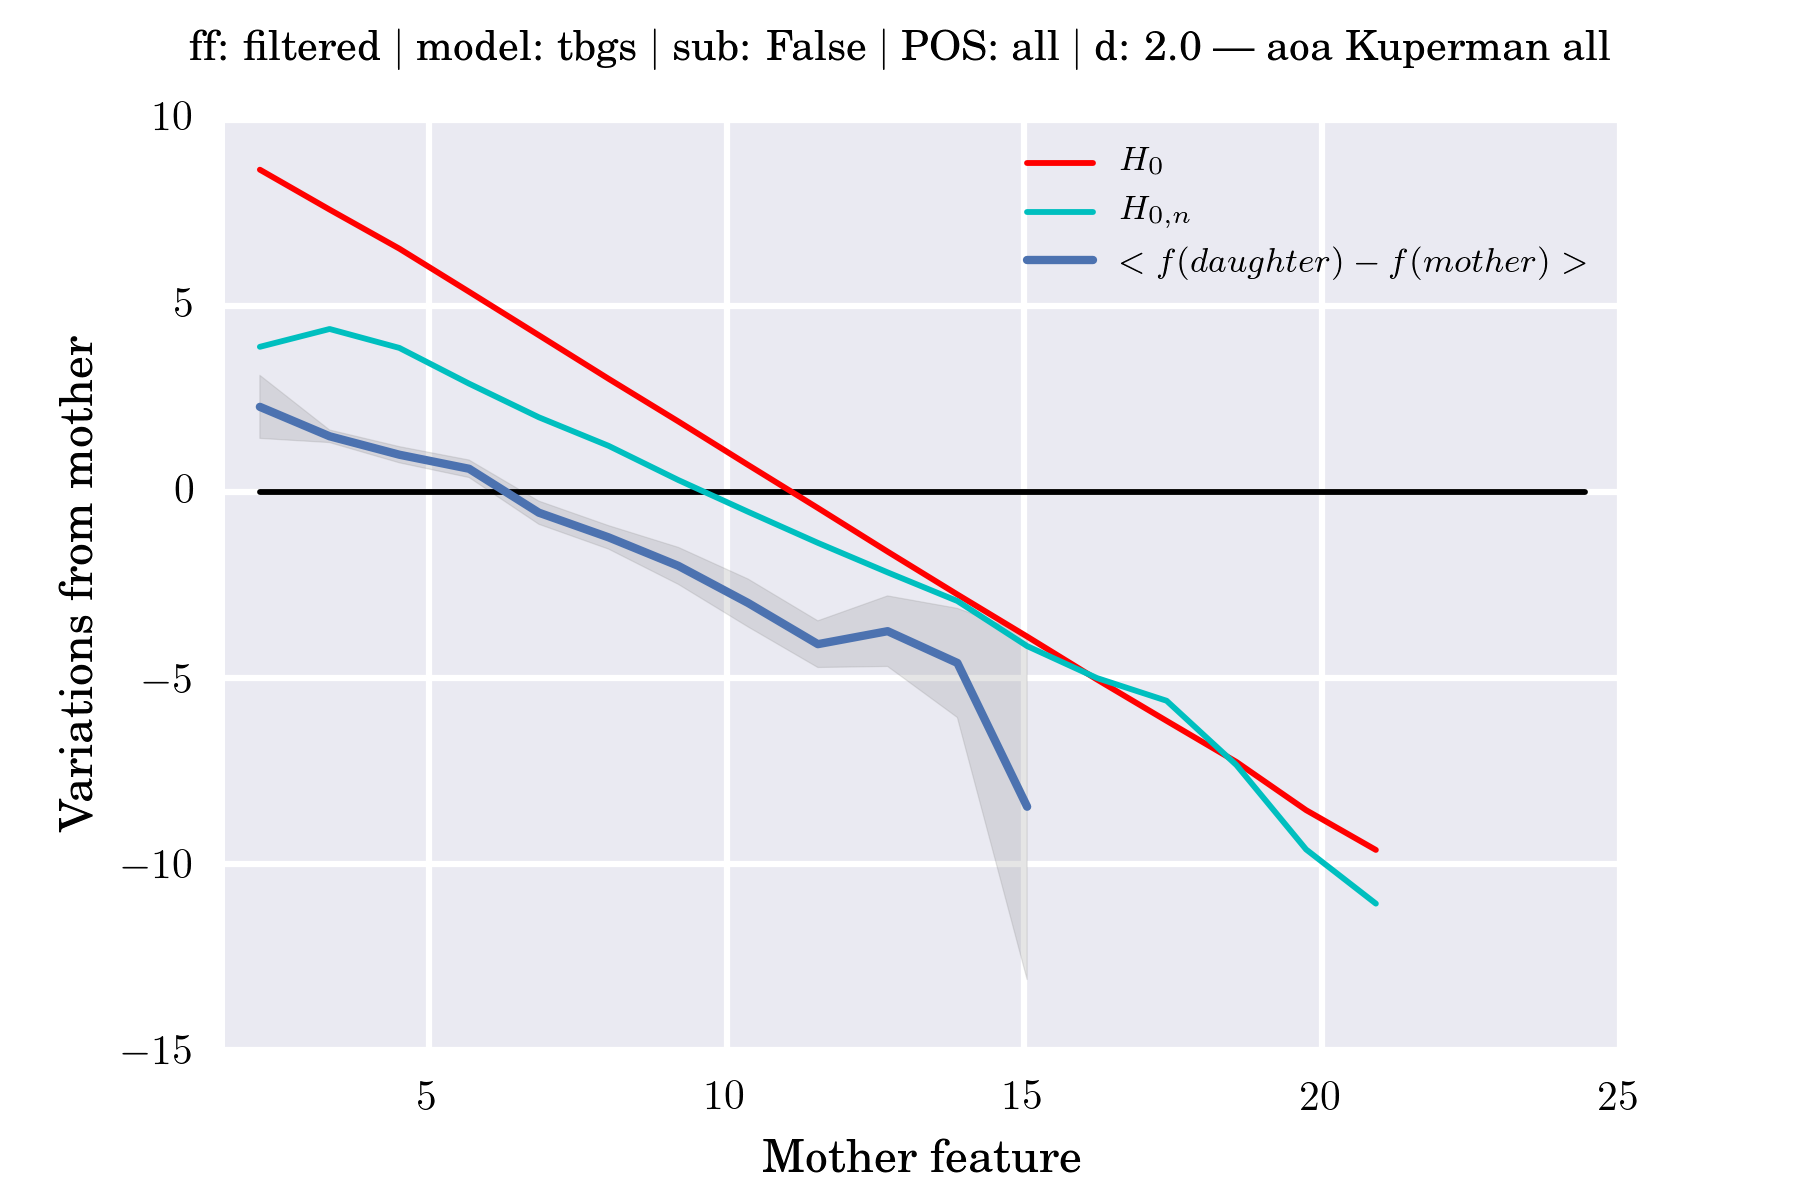
\includegraphics[width=0.6\textwidth]{images/feature-cards/aoa_Kuperman/feature_variations.png}
    \caption{Feature variation on substitution}
	\subfloat[][Scatter plot]{
		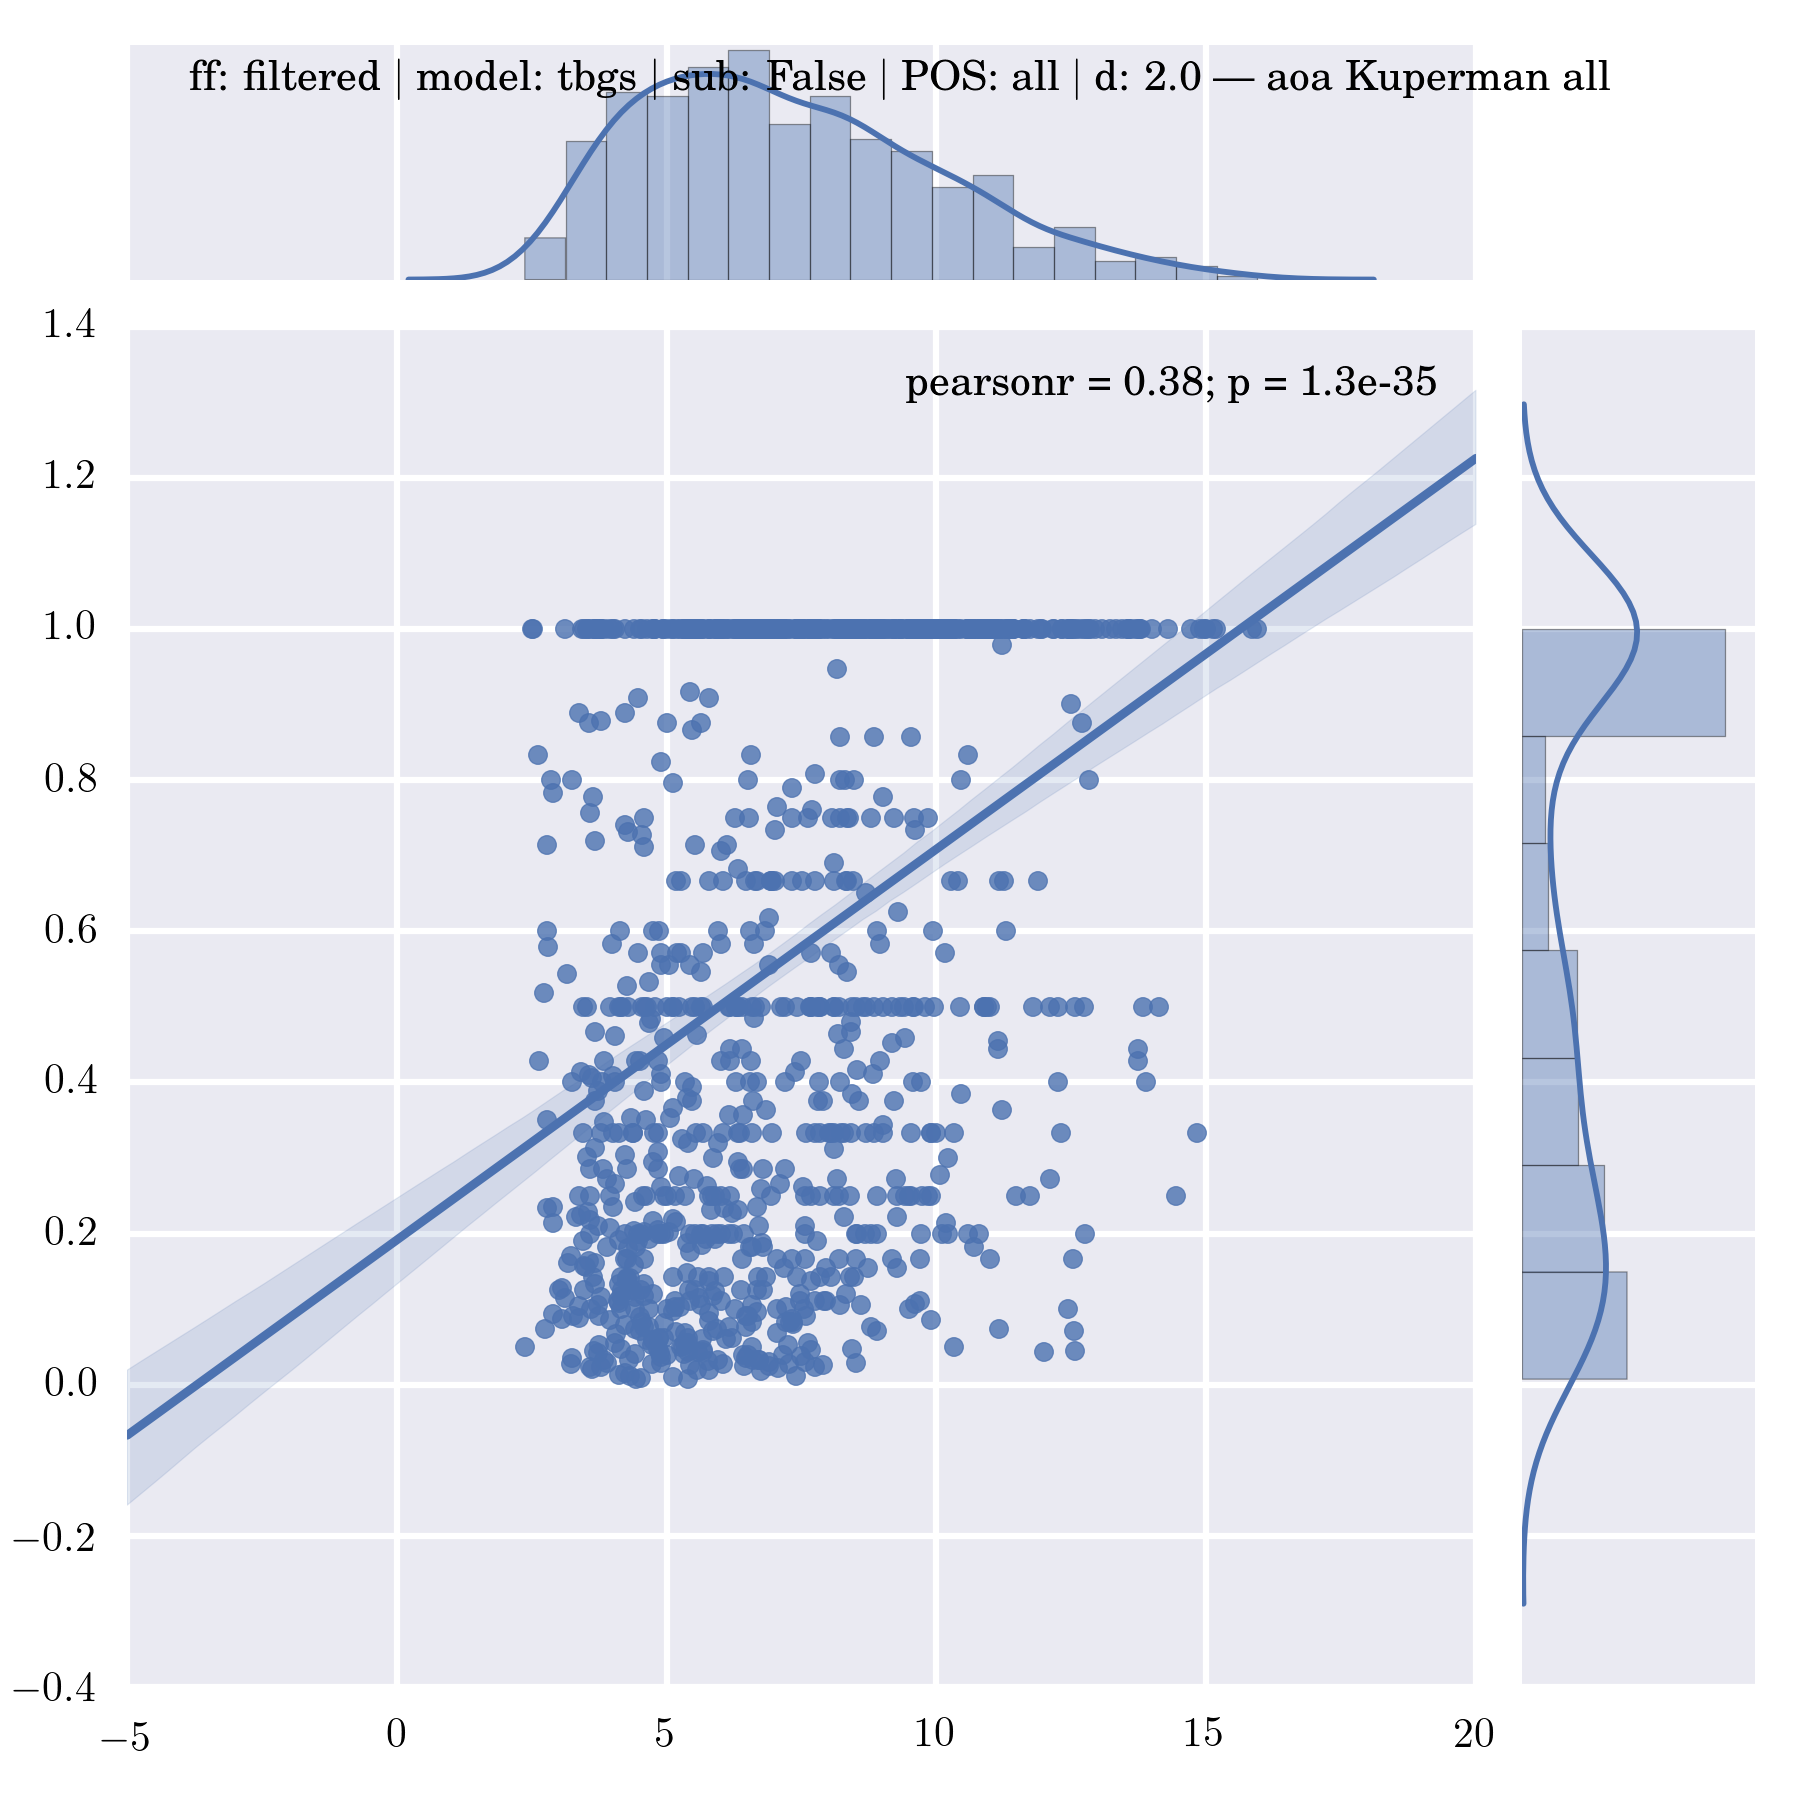
\includegraphics[width=0.3\textwidth]{images/feature-cards/aoa_Kuperman/susceptibility_scatter.png}
	}
	~
	\subfloat[][Bin averages and KDE]{
		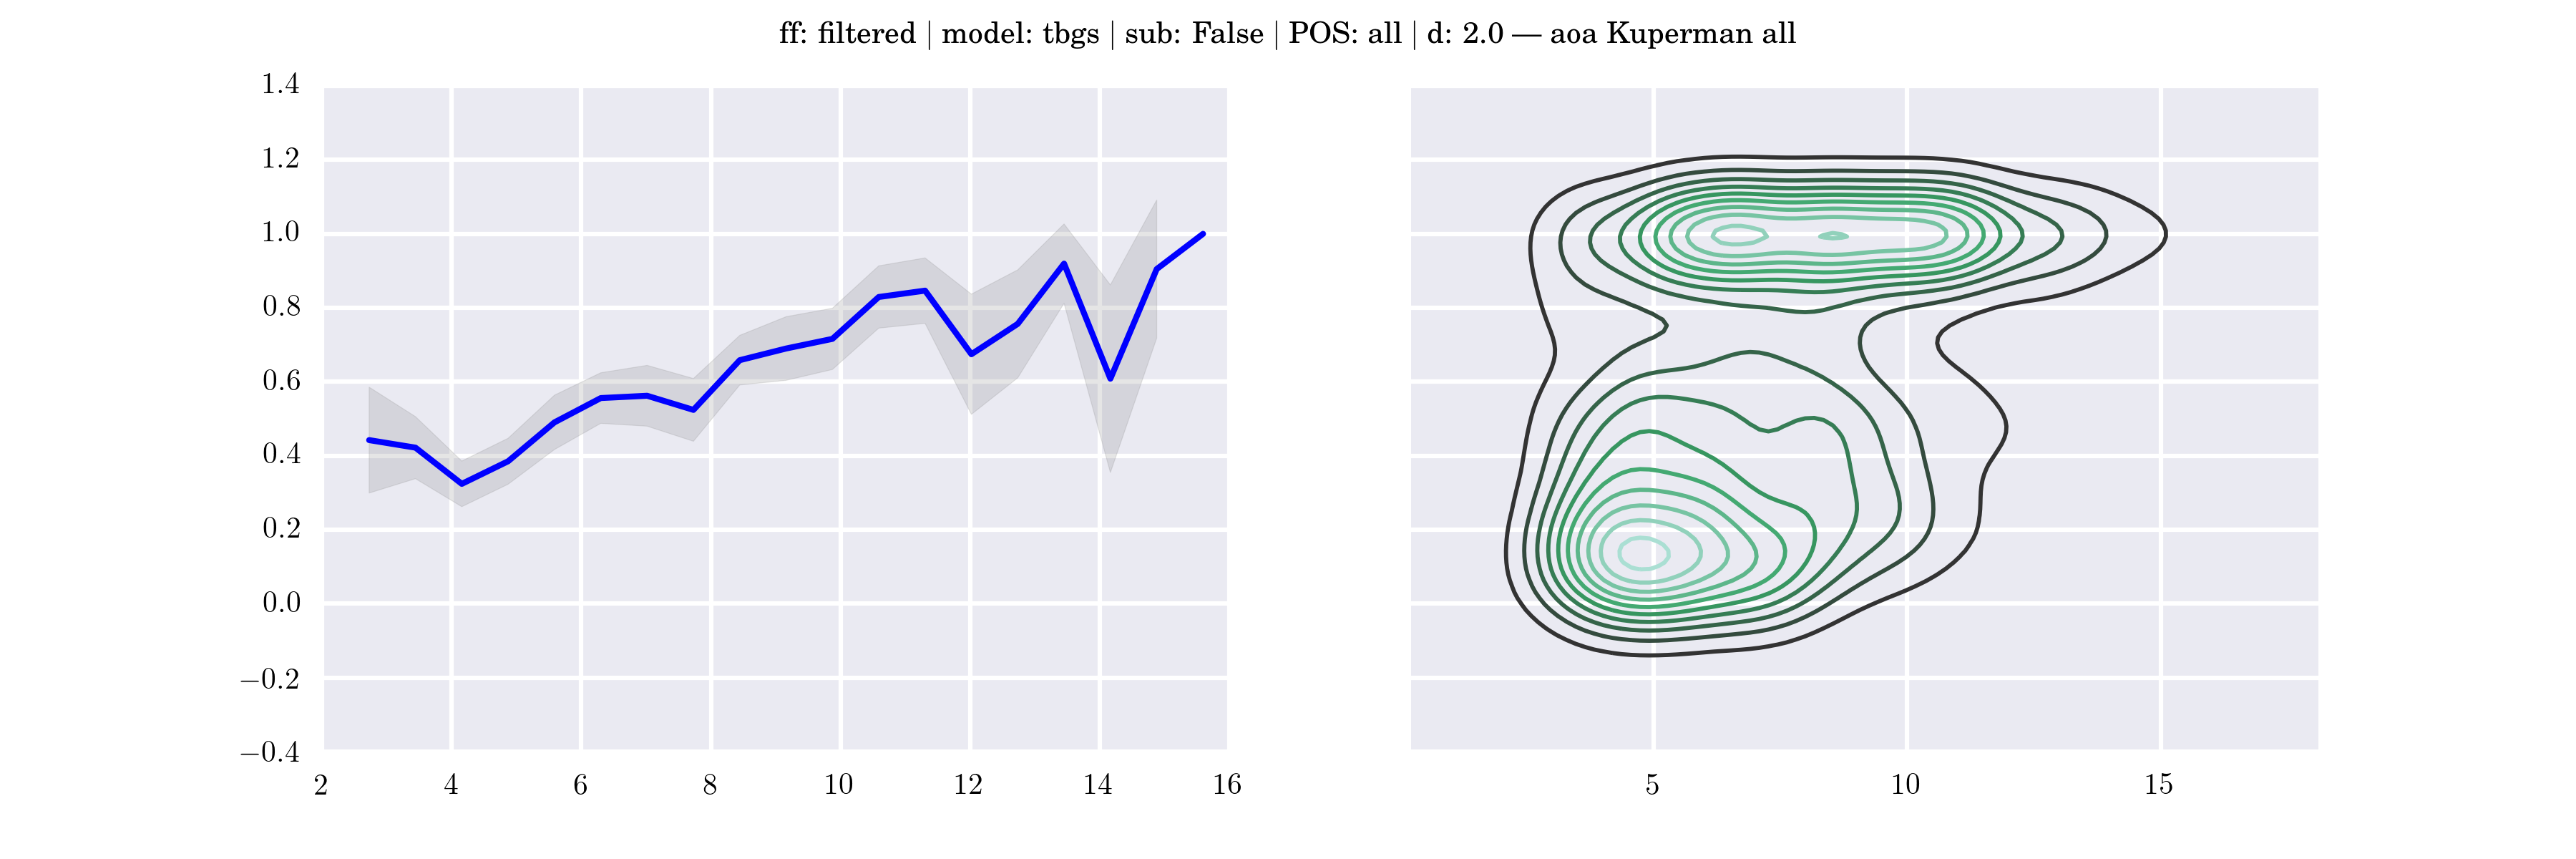
\includegraphics[width=0.6\textwidth]{images/feature-cards/aoa_Kuperman/susceptibility.png}
	}
	\caption{Substitution susceptibility}
    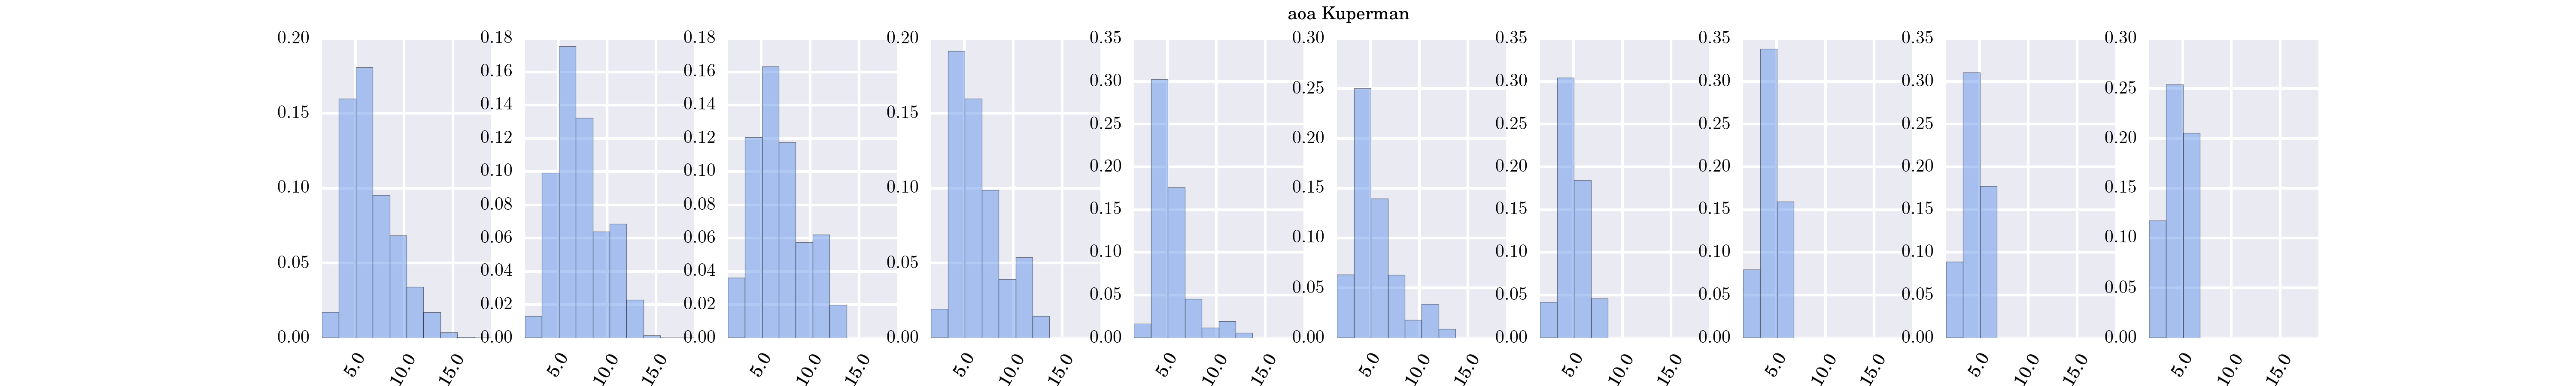
\includegraphics[width=\textwidth]{images/feature-cards/aoa_Kuperman/timebags_evolution-hist.png}
	\caption{Timebag evolution}
\end{figure*}


% cmu_MNphonemes ===============================
\clearpage
\subsection{cmu MNphonemes}
\begin{figure*}[h!]
    \centering
    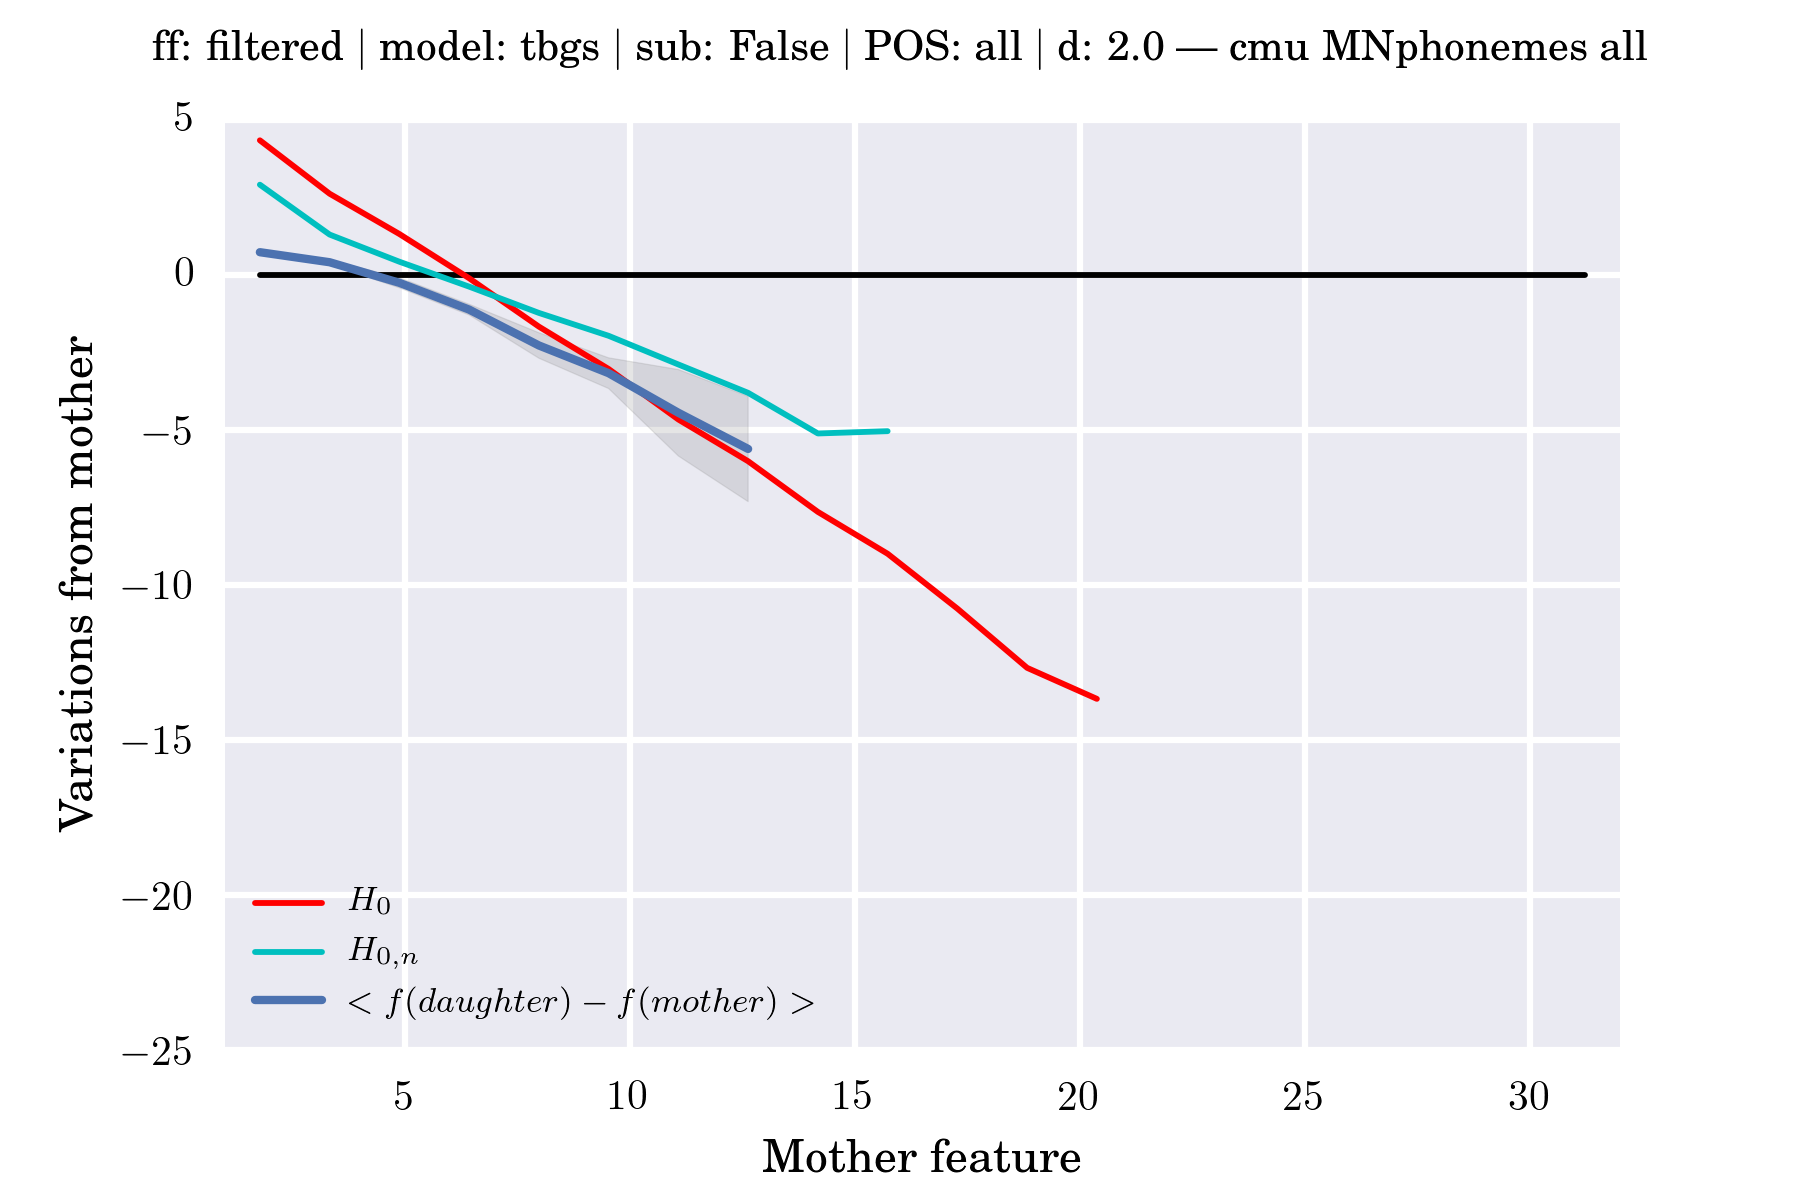
\includegraphics[width=0.6\textwidth]{images/feature-cards/cmu_MNphonemes/feature_variations.png}
    \caption{Feature variation on substitution}
	\subfloat[][Scatter plot]{
		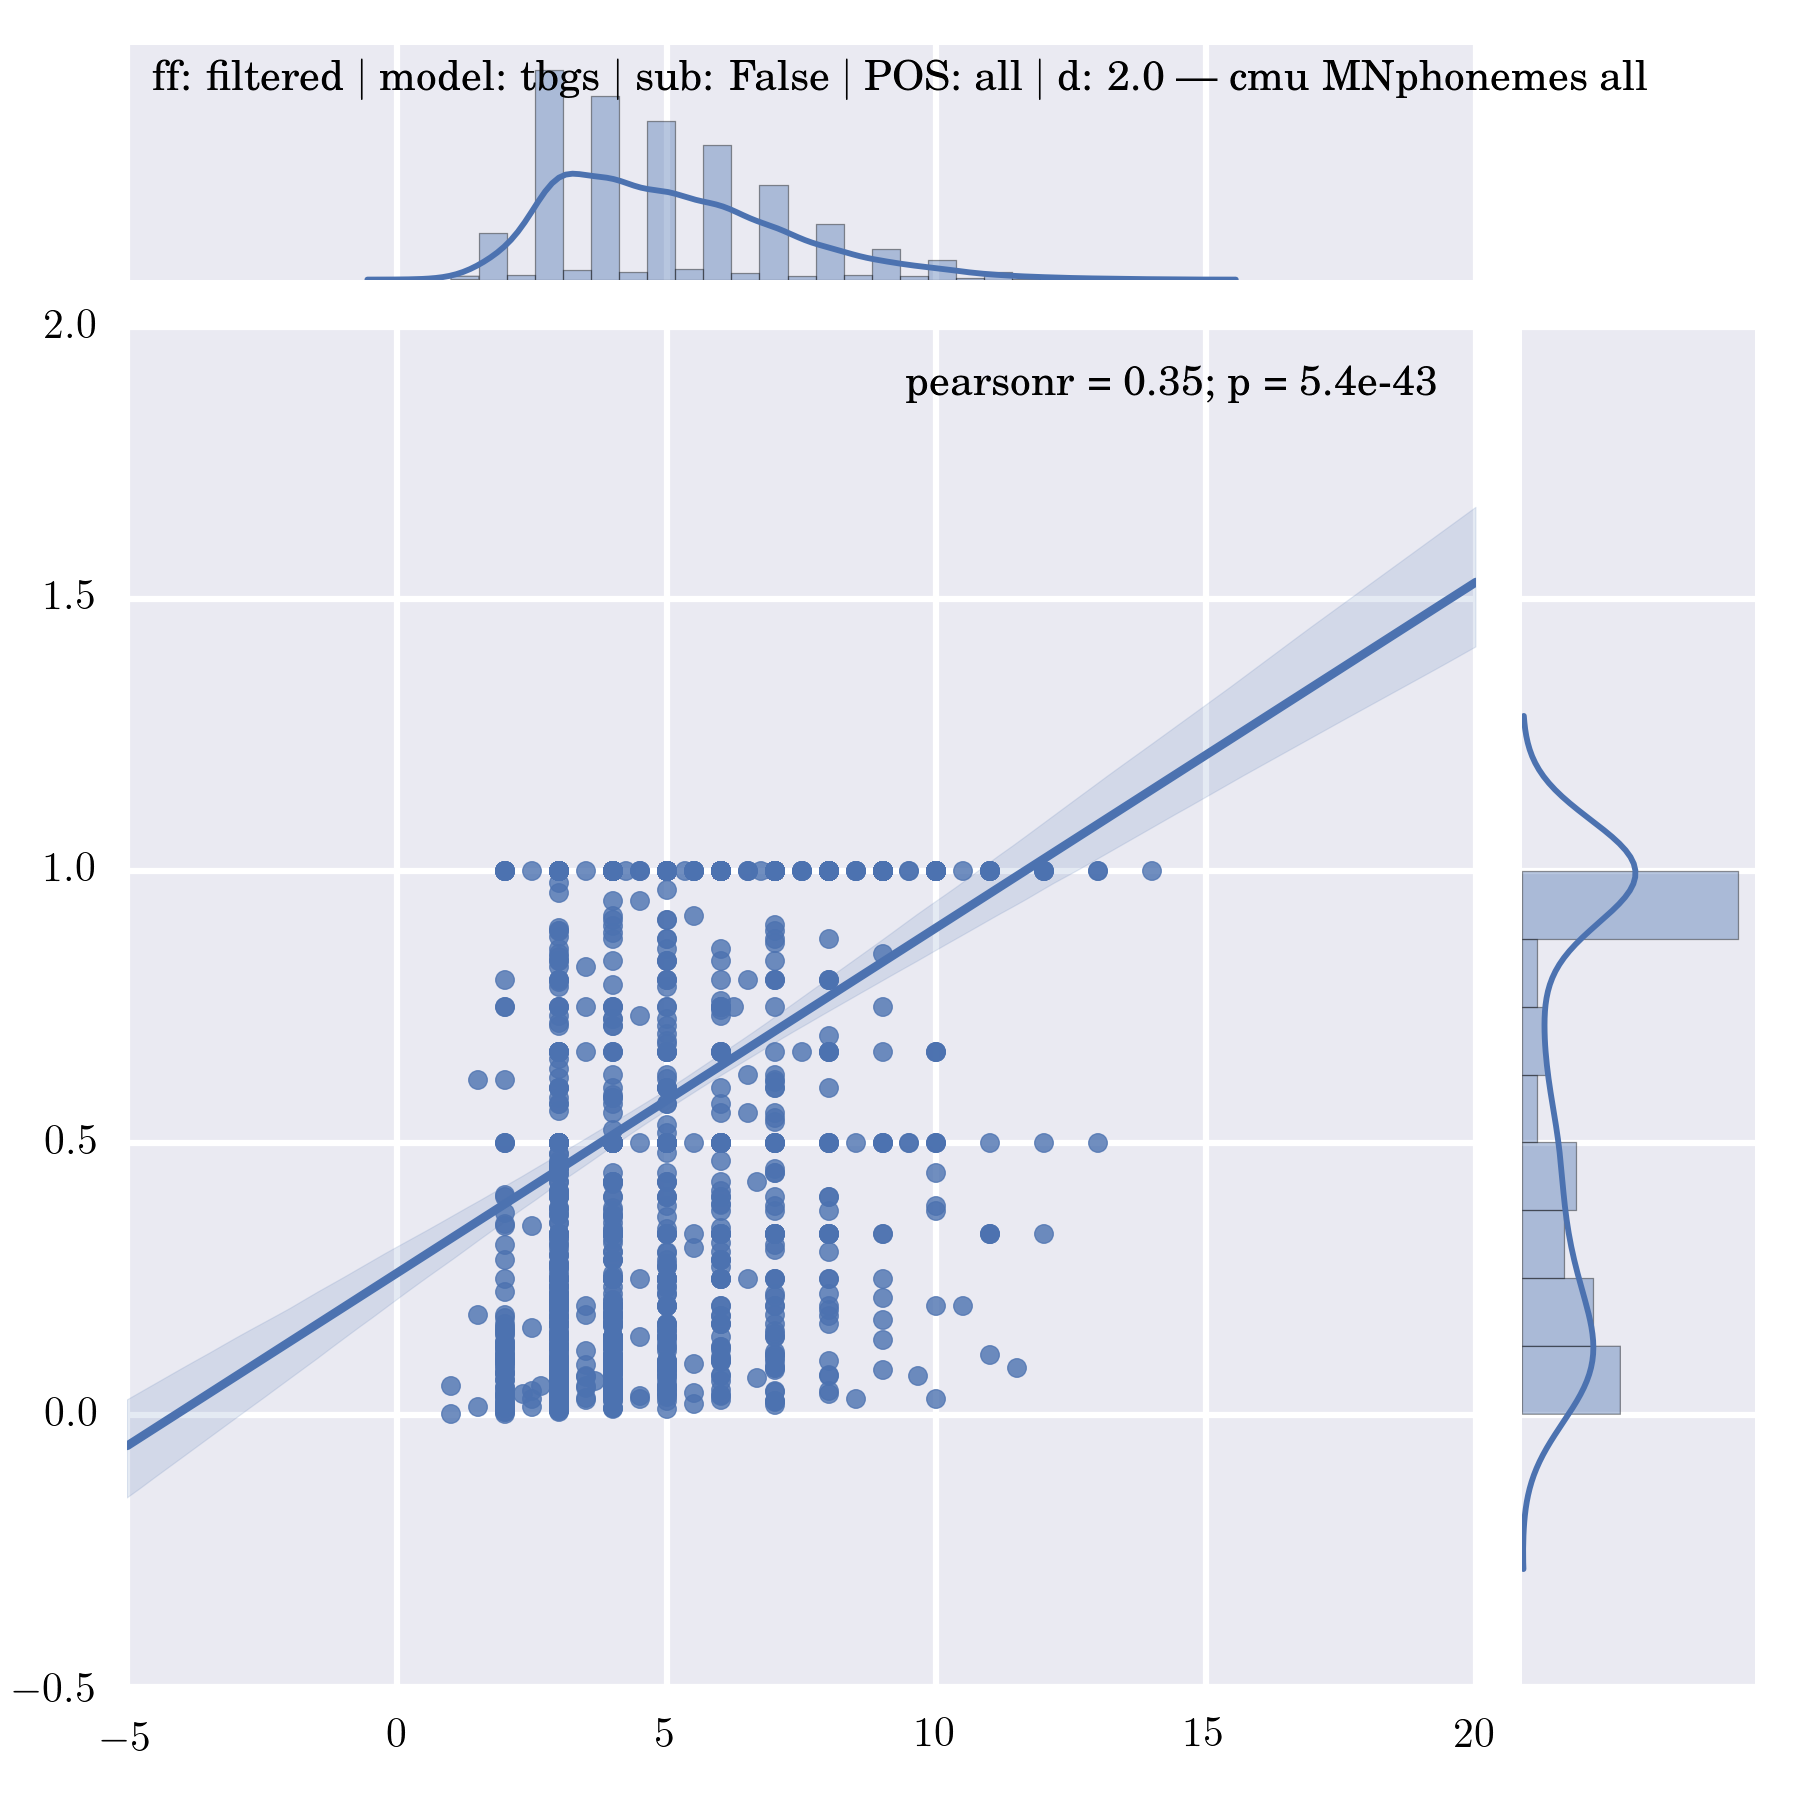
\includegraphics[width=0.3\textwidth]{images/feature-cards/cmu_MNphonemes/susceptibility_scatter.png}
	}
	~
	\subfloat[][Bin averages and KDE]{
		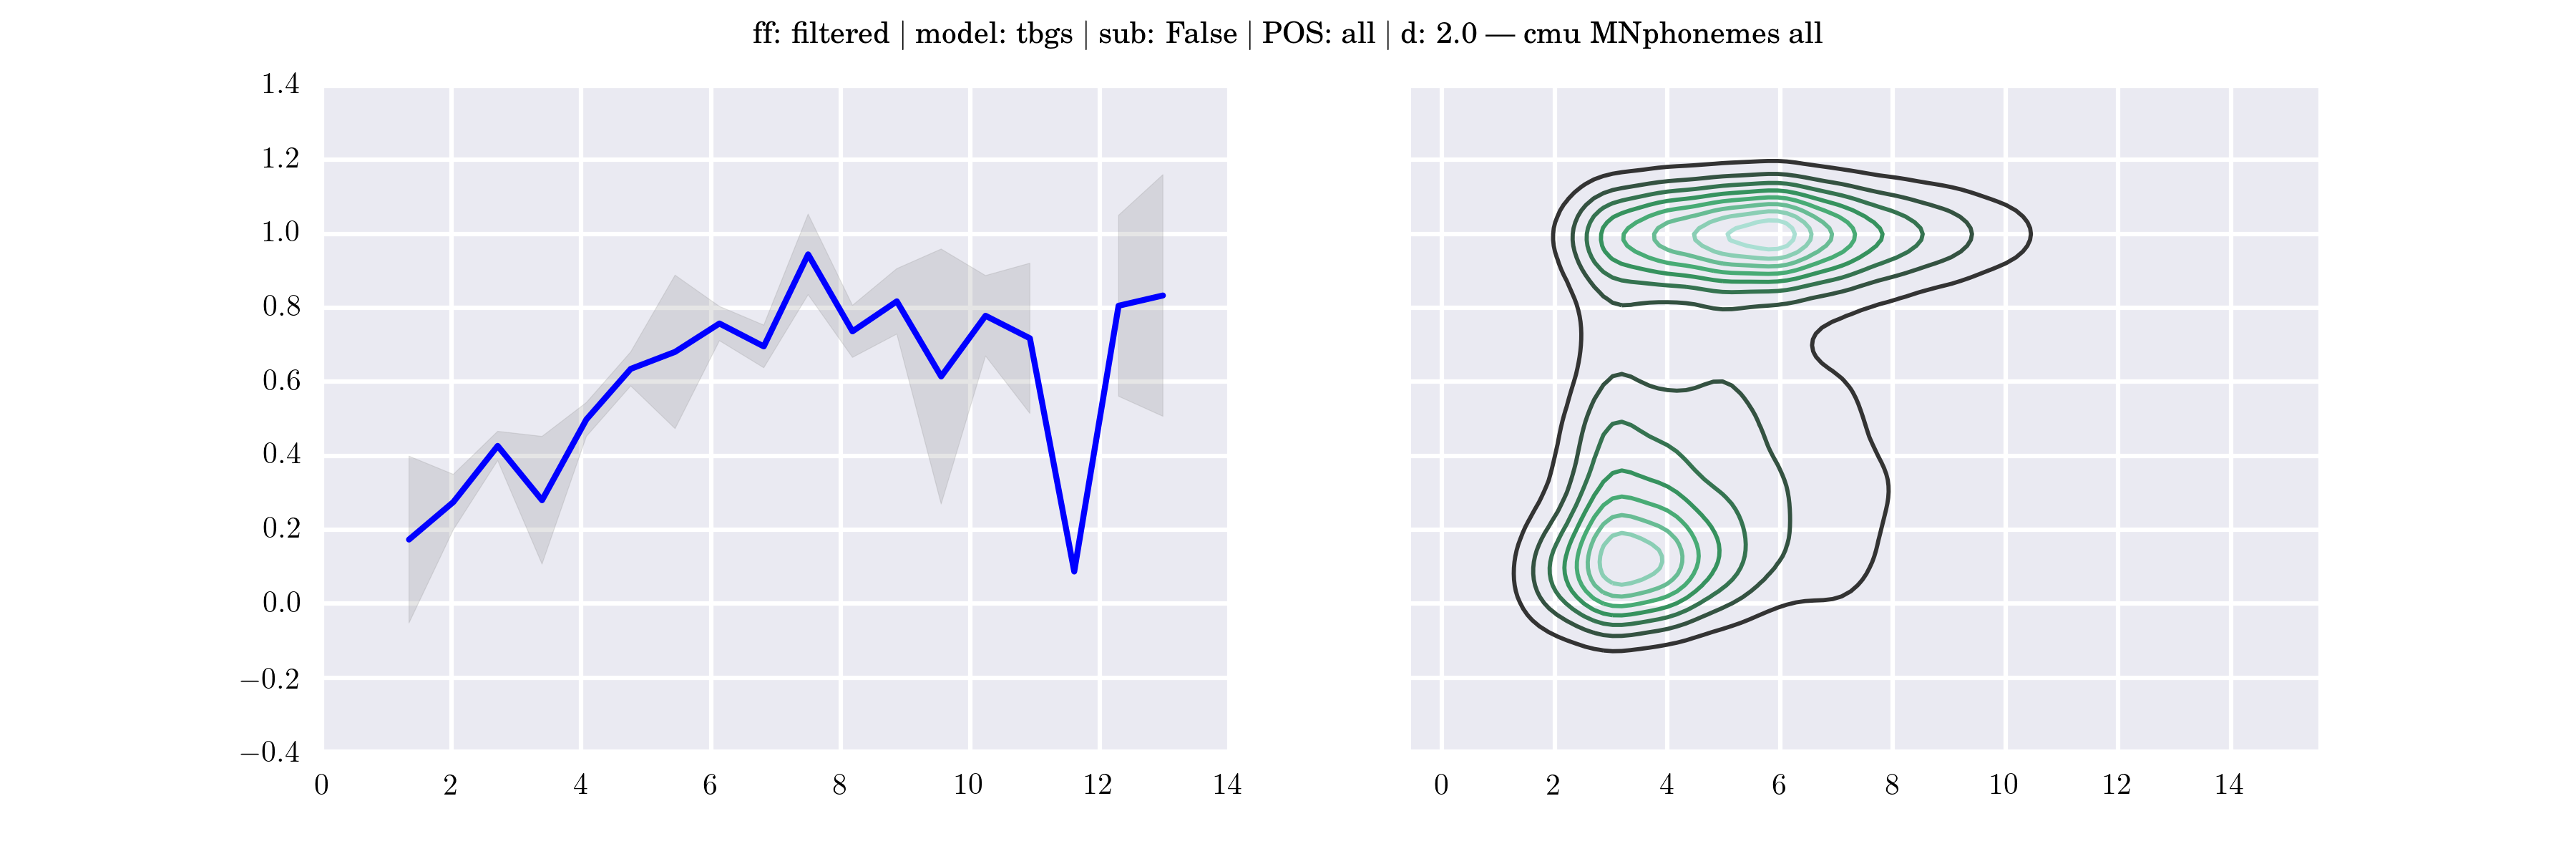
\includegraphics[width=0.6\textwidth]{images/feature-cards/cmu_MNphonemes/susceptibility.png}
	}
	\caption{Substitution susceptibility}
    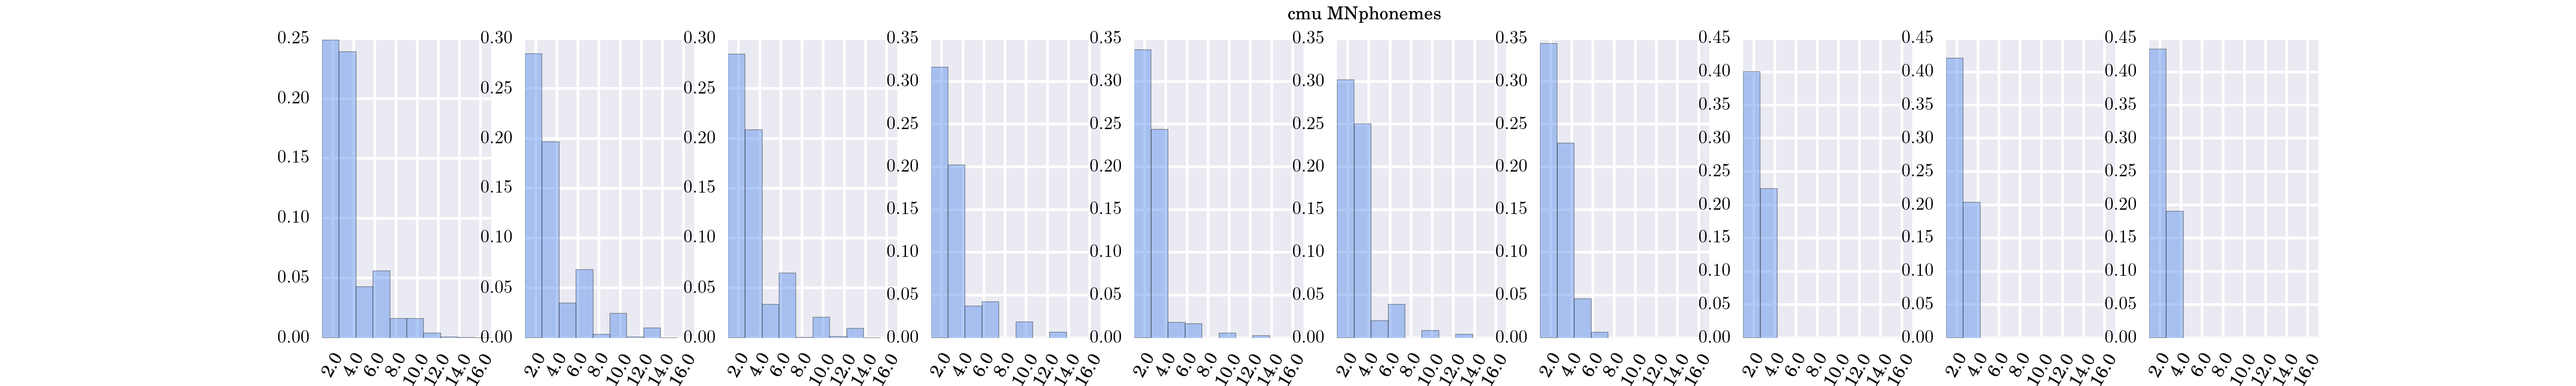
\includegraphics[width=\textwidth]{images/feature-cards/cmu_MNphonemes/timebags_evolution-hist.png}
	\caption{Timebag evolution}
\end{figure*}


% cmu_MNsyllables ===============================
\clearpage
\subsection{cmu MNsyllables}
\begin{figure*}[h!]
    \centering
    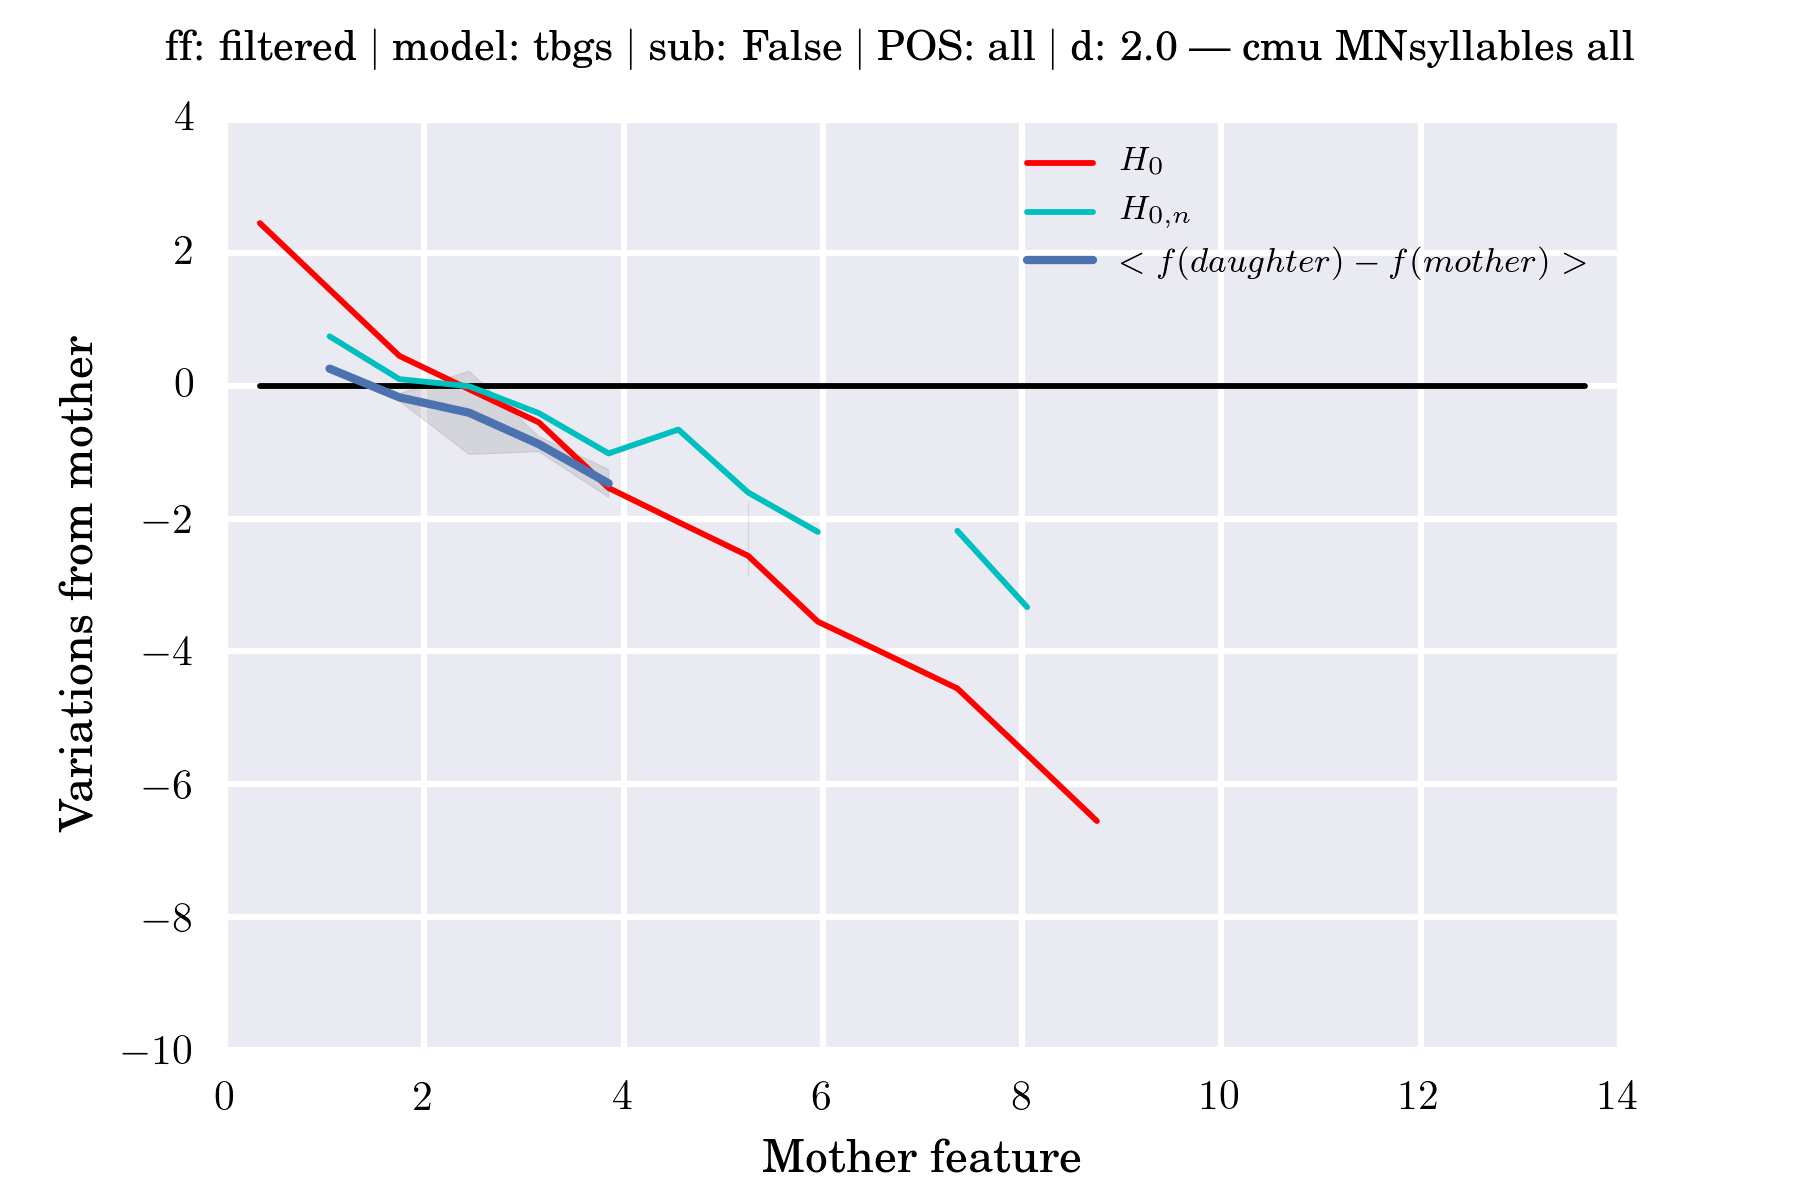
\includegraphics[width=0.6\textwidth]{images/feature-cards/cmu_MNsyllables/feature_variations.png}
    \caption{Feature variation on substitution}
	\subfloat[][Scatter plot]{
		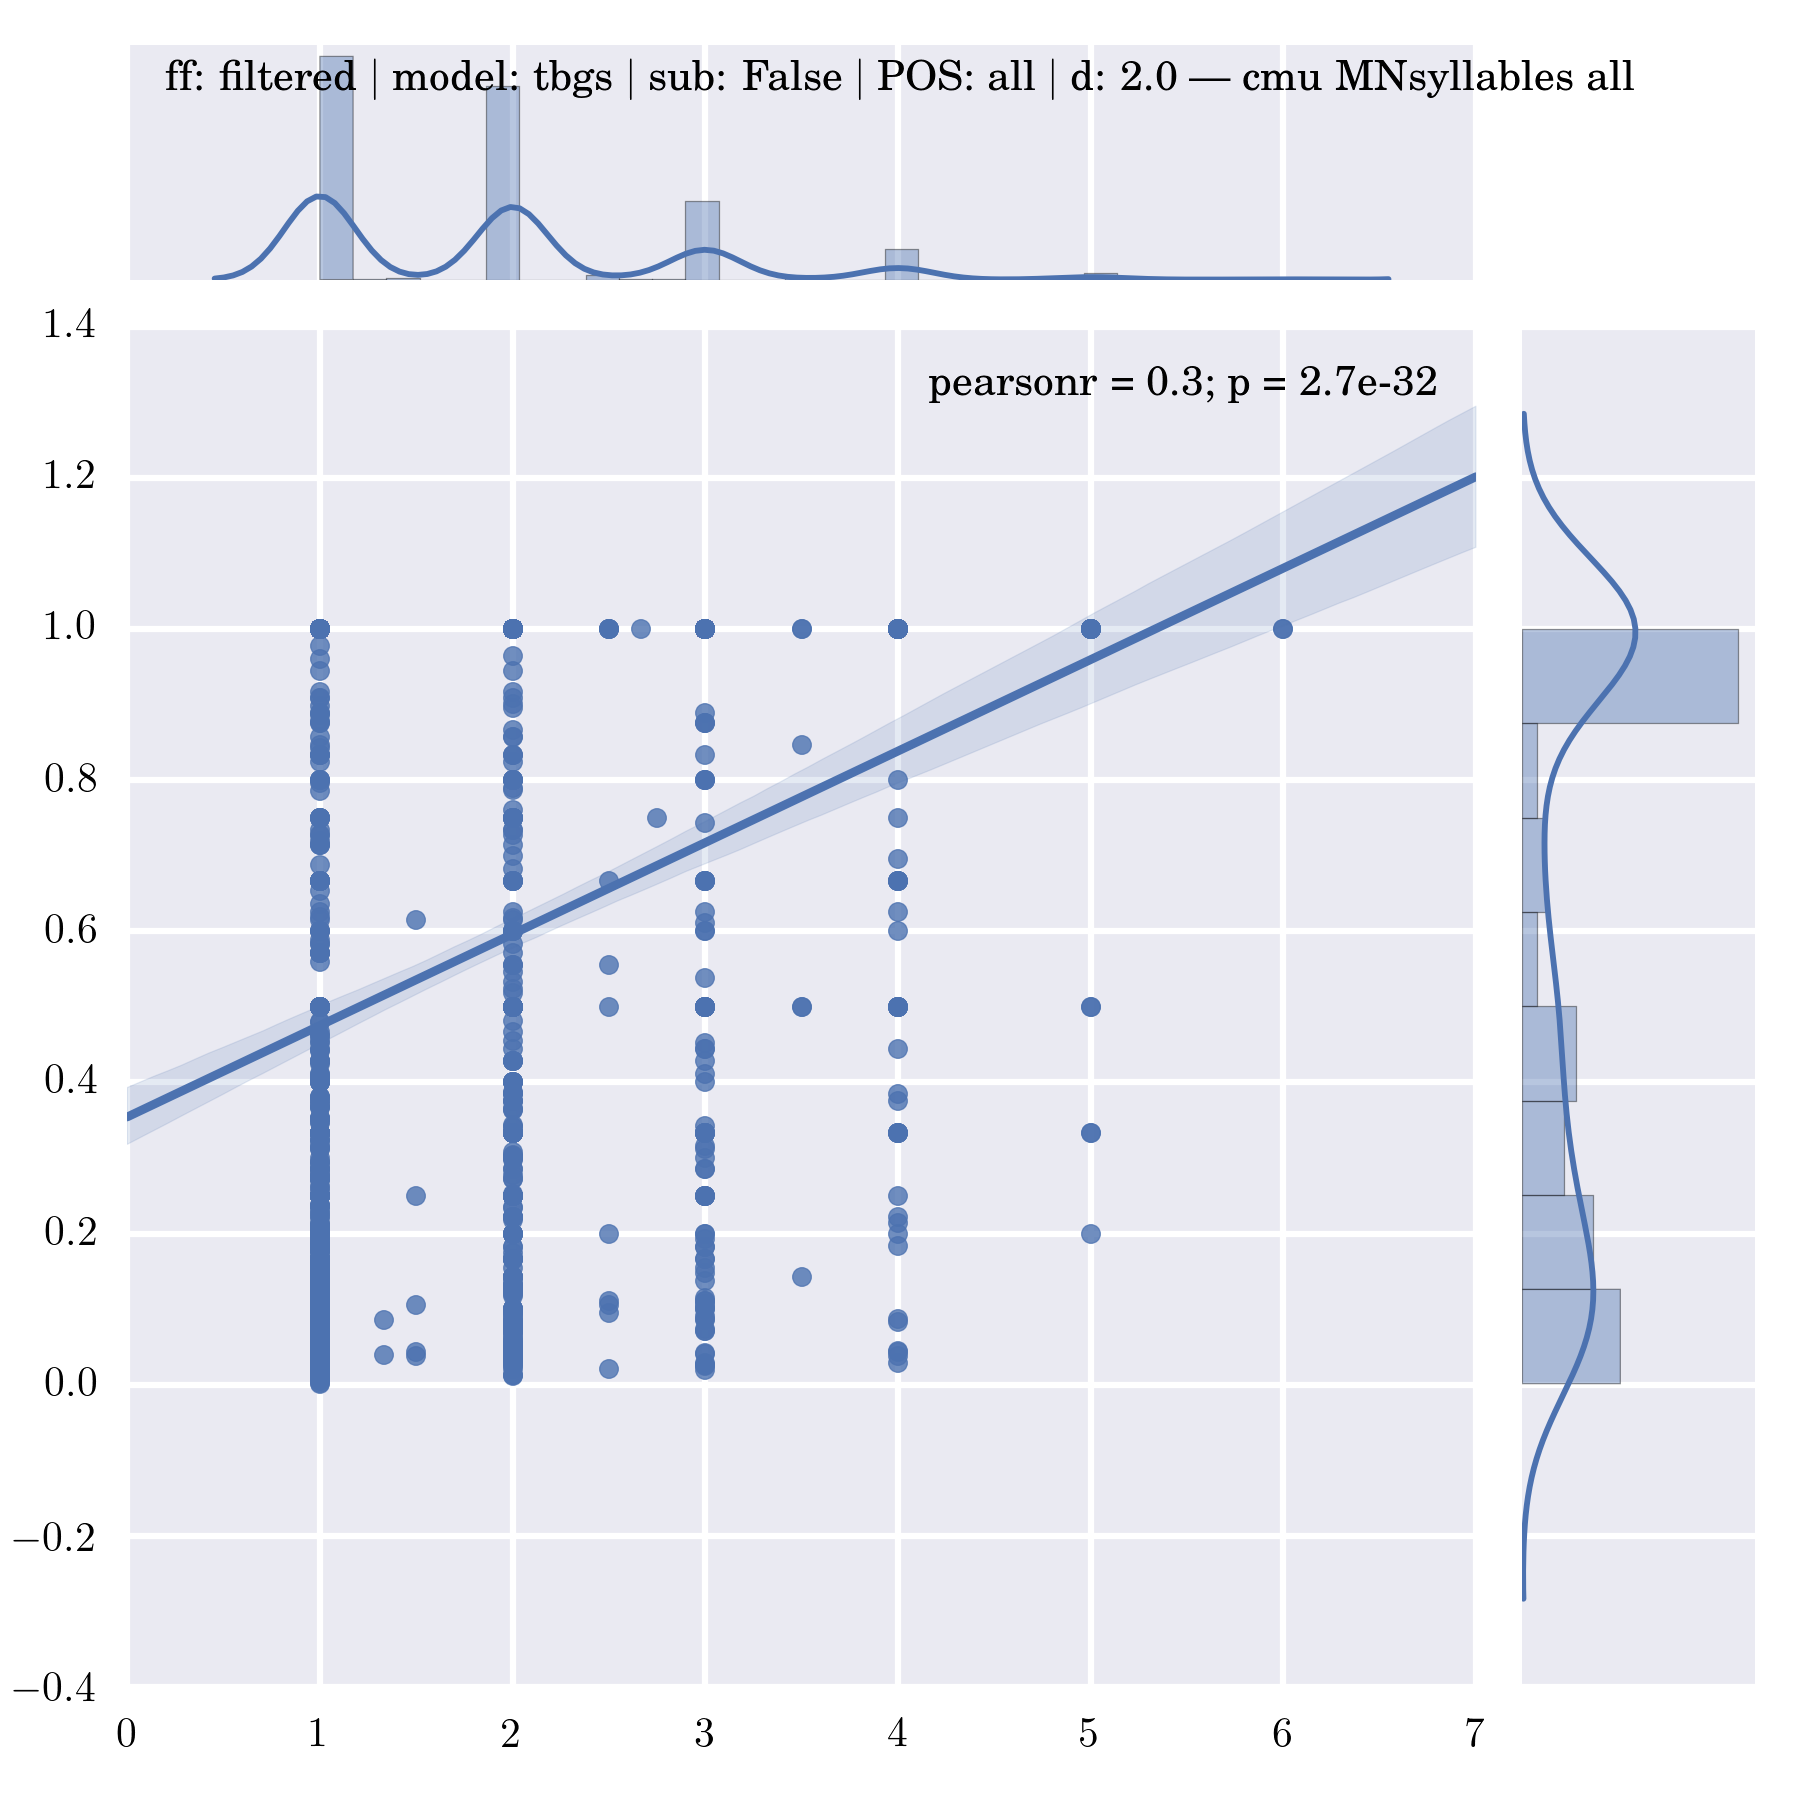
\includegraphics[width=0.3\textwidth]{images/feature-cards/cmu_MNsyllables/susceptibility_scatter.png}
	}
	~
	\subfloat[][Bin averages and KDE]{
		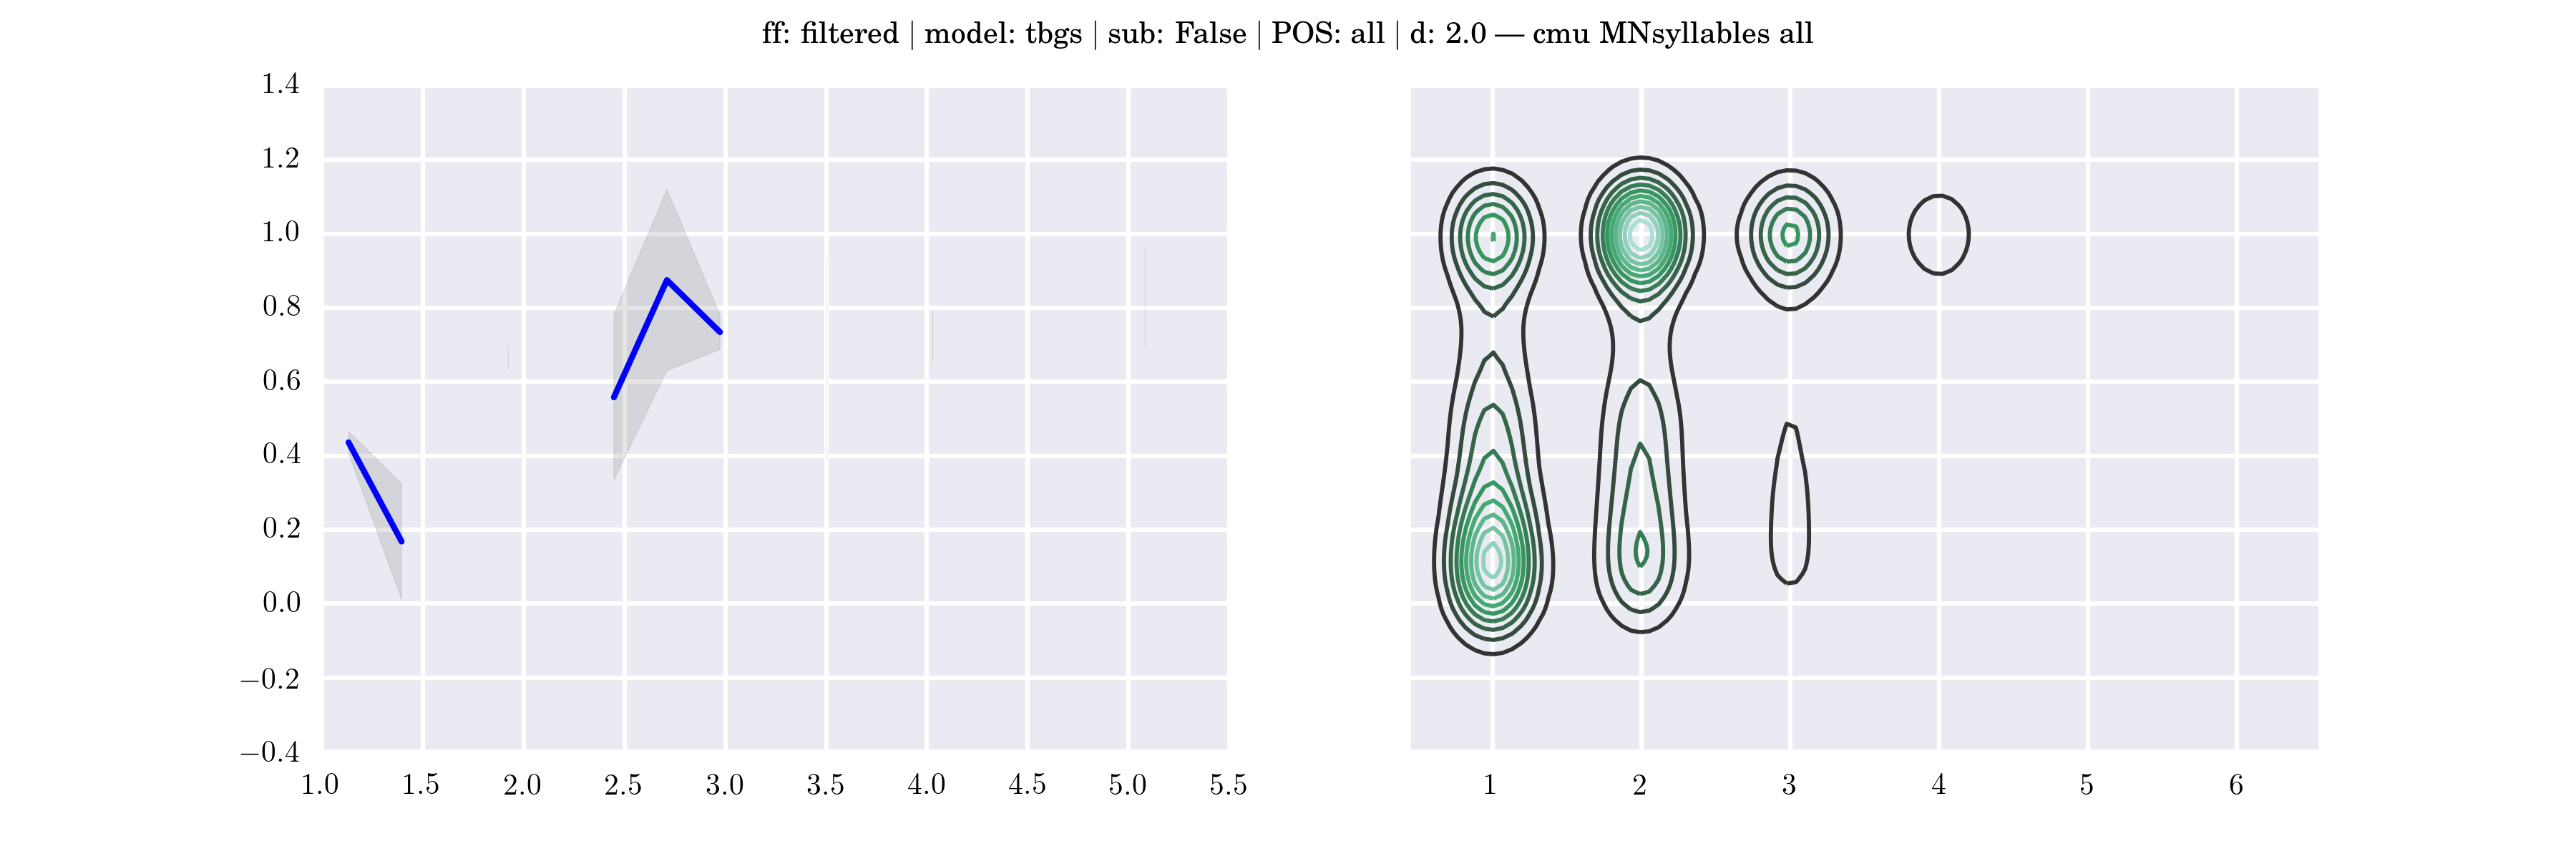
\includegraphics[width=0.6\textwidth]{images/feature-cards/cmu_MNsyllables/susceptibility.png}
	}
	\caption{Substitution susceptibility}
    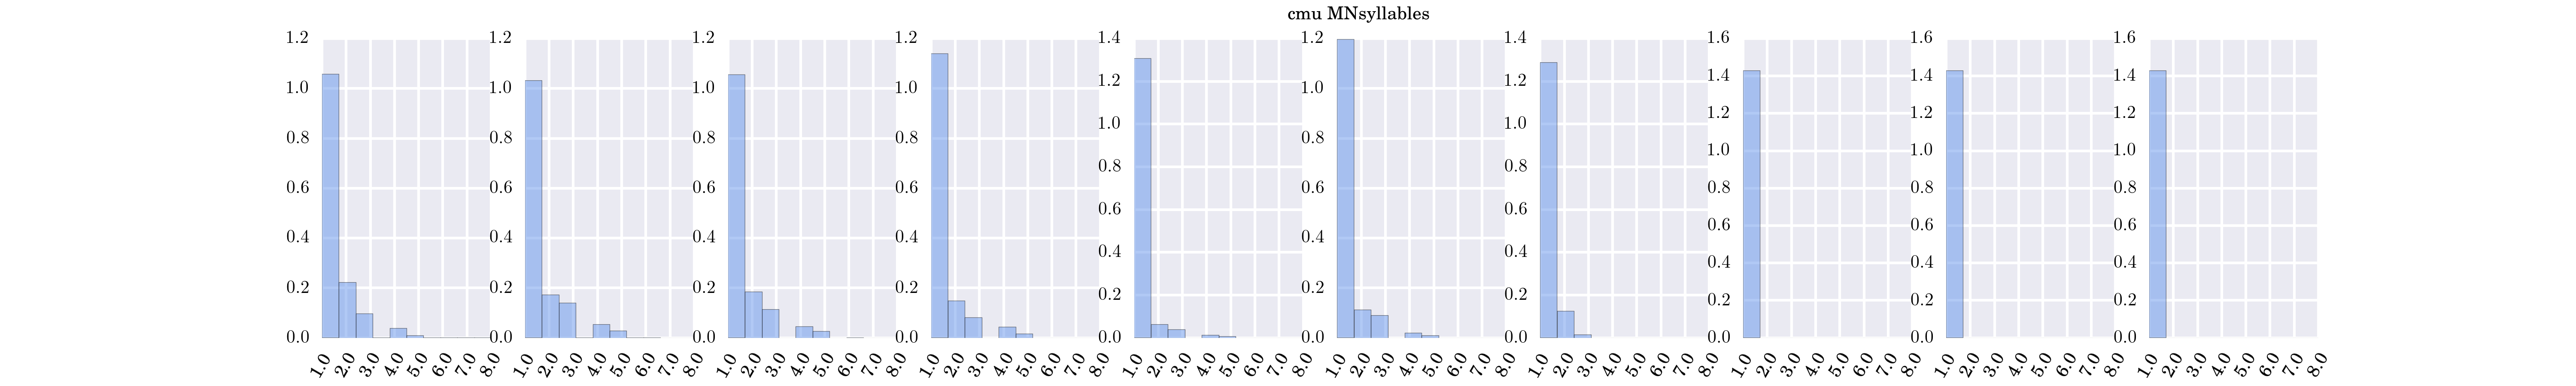
\includegraphics[width=\textwidth]{images/feature-cards/cmu_MNsyllables/timebags_evolution-hist.png}
	\caption{Timebag evolution}
\end{figure*}


% fa_BCs ===============================
\clearpage
\subsection{fa BCs}
\begin{figure*}[h!]
    \centering
    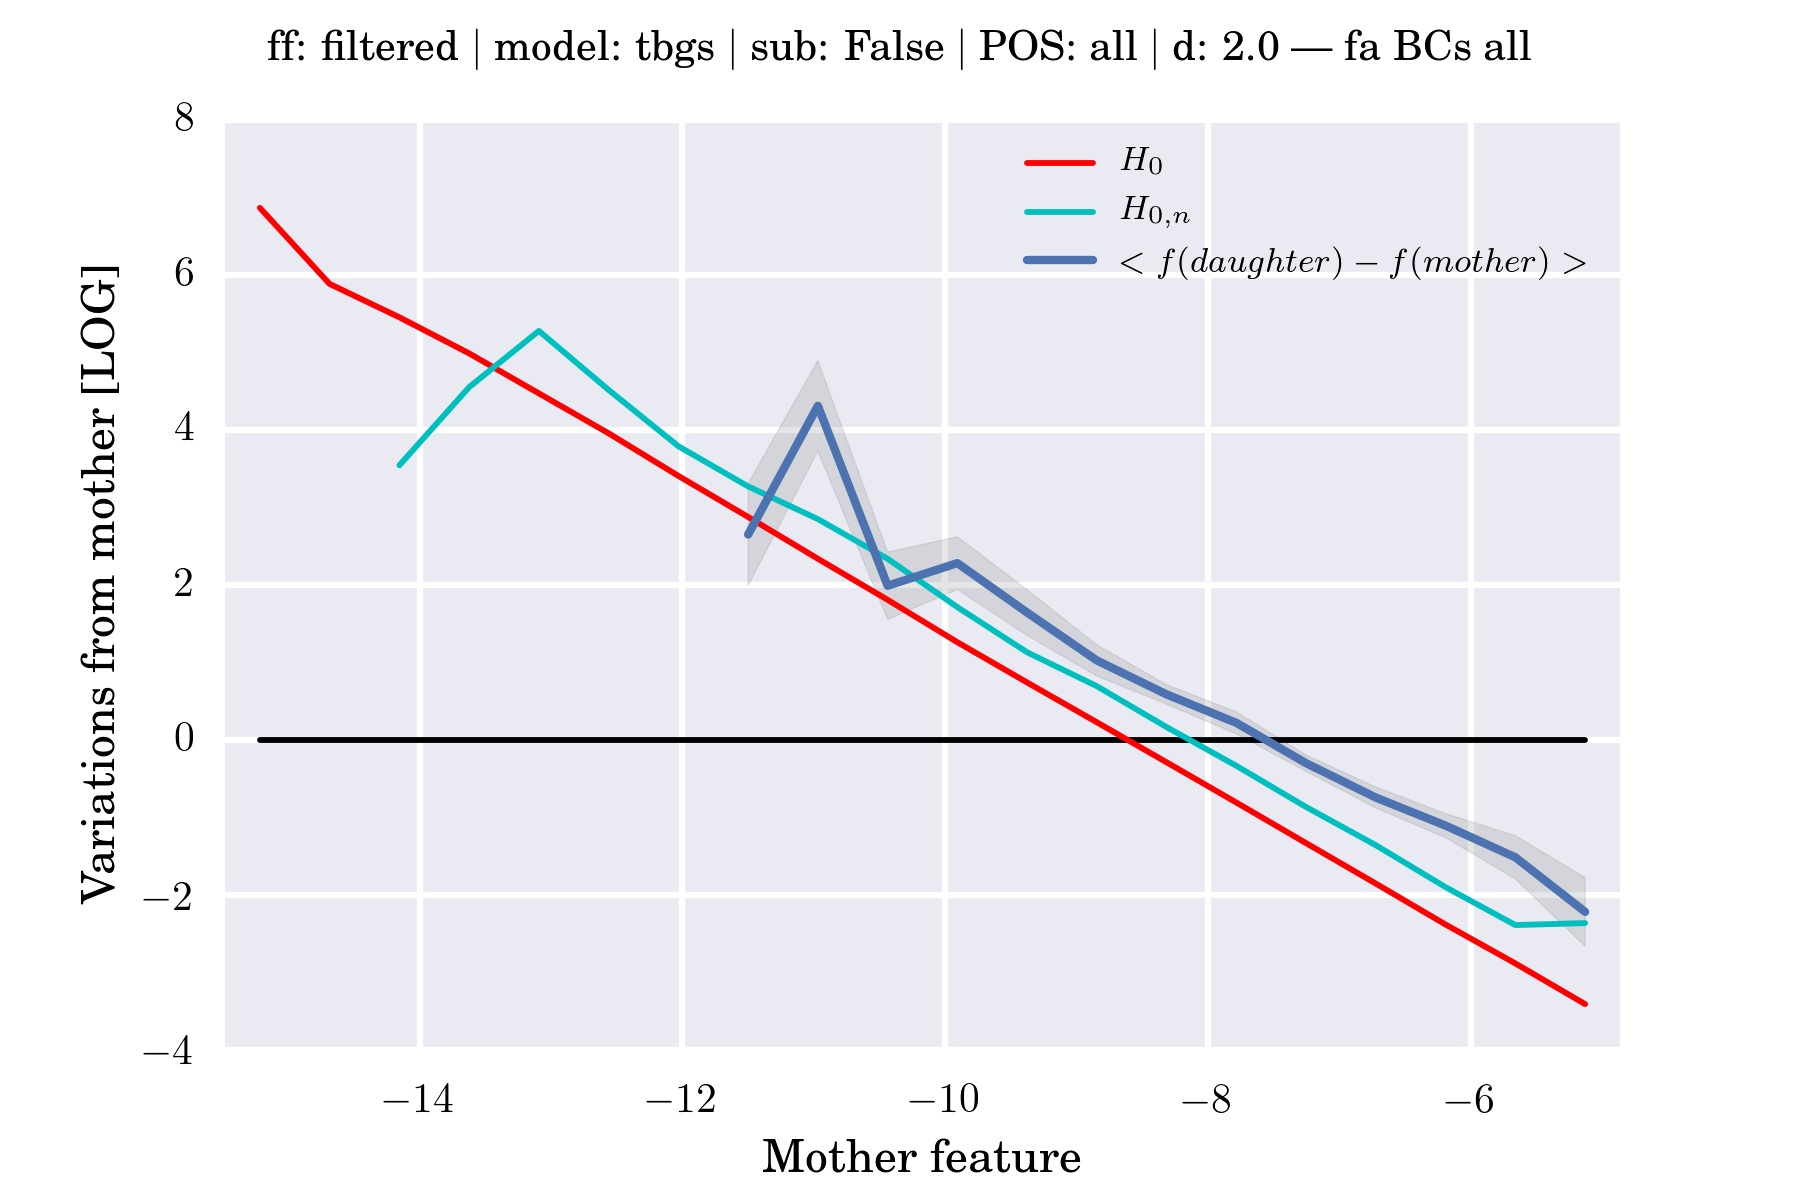
\includegraphics[width=0.6\textwidth]{images/feature-cards/fa_BCs/feature_variations.png}
    \caption{Feature variation on substitution}
	\subfloat[][Scatter plot]{
		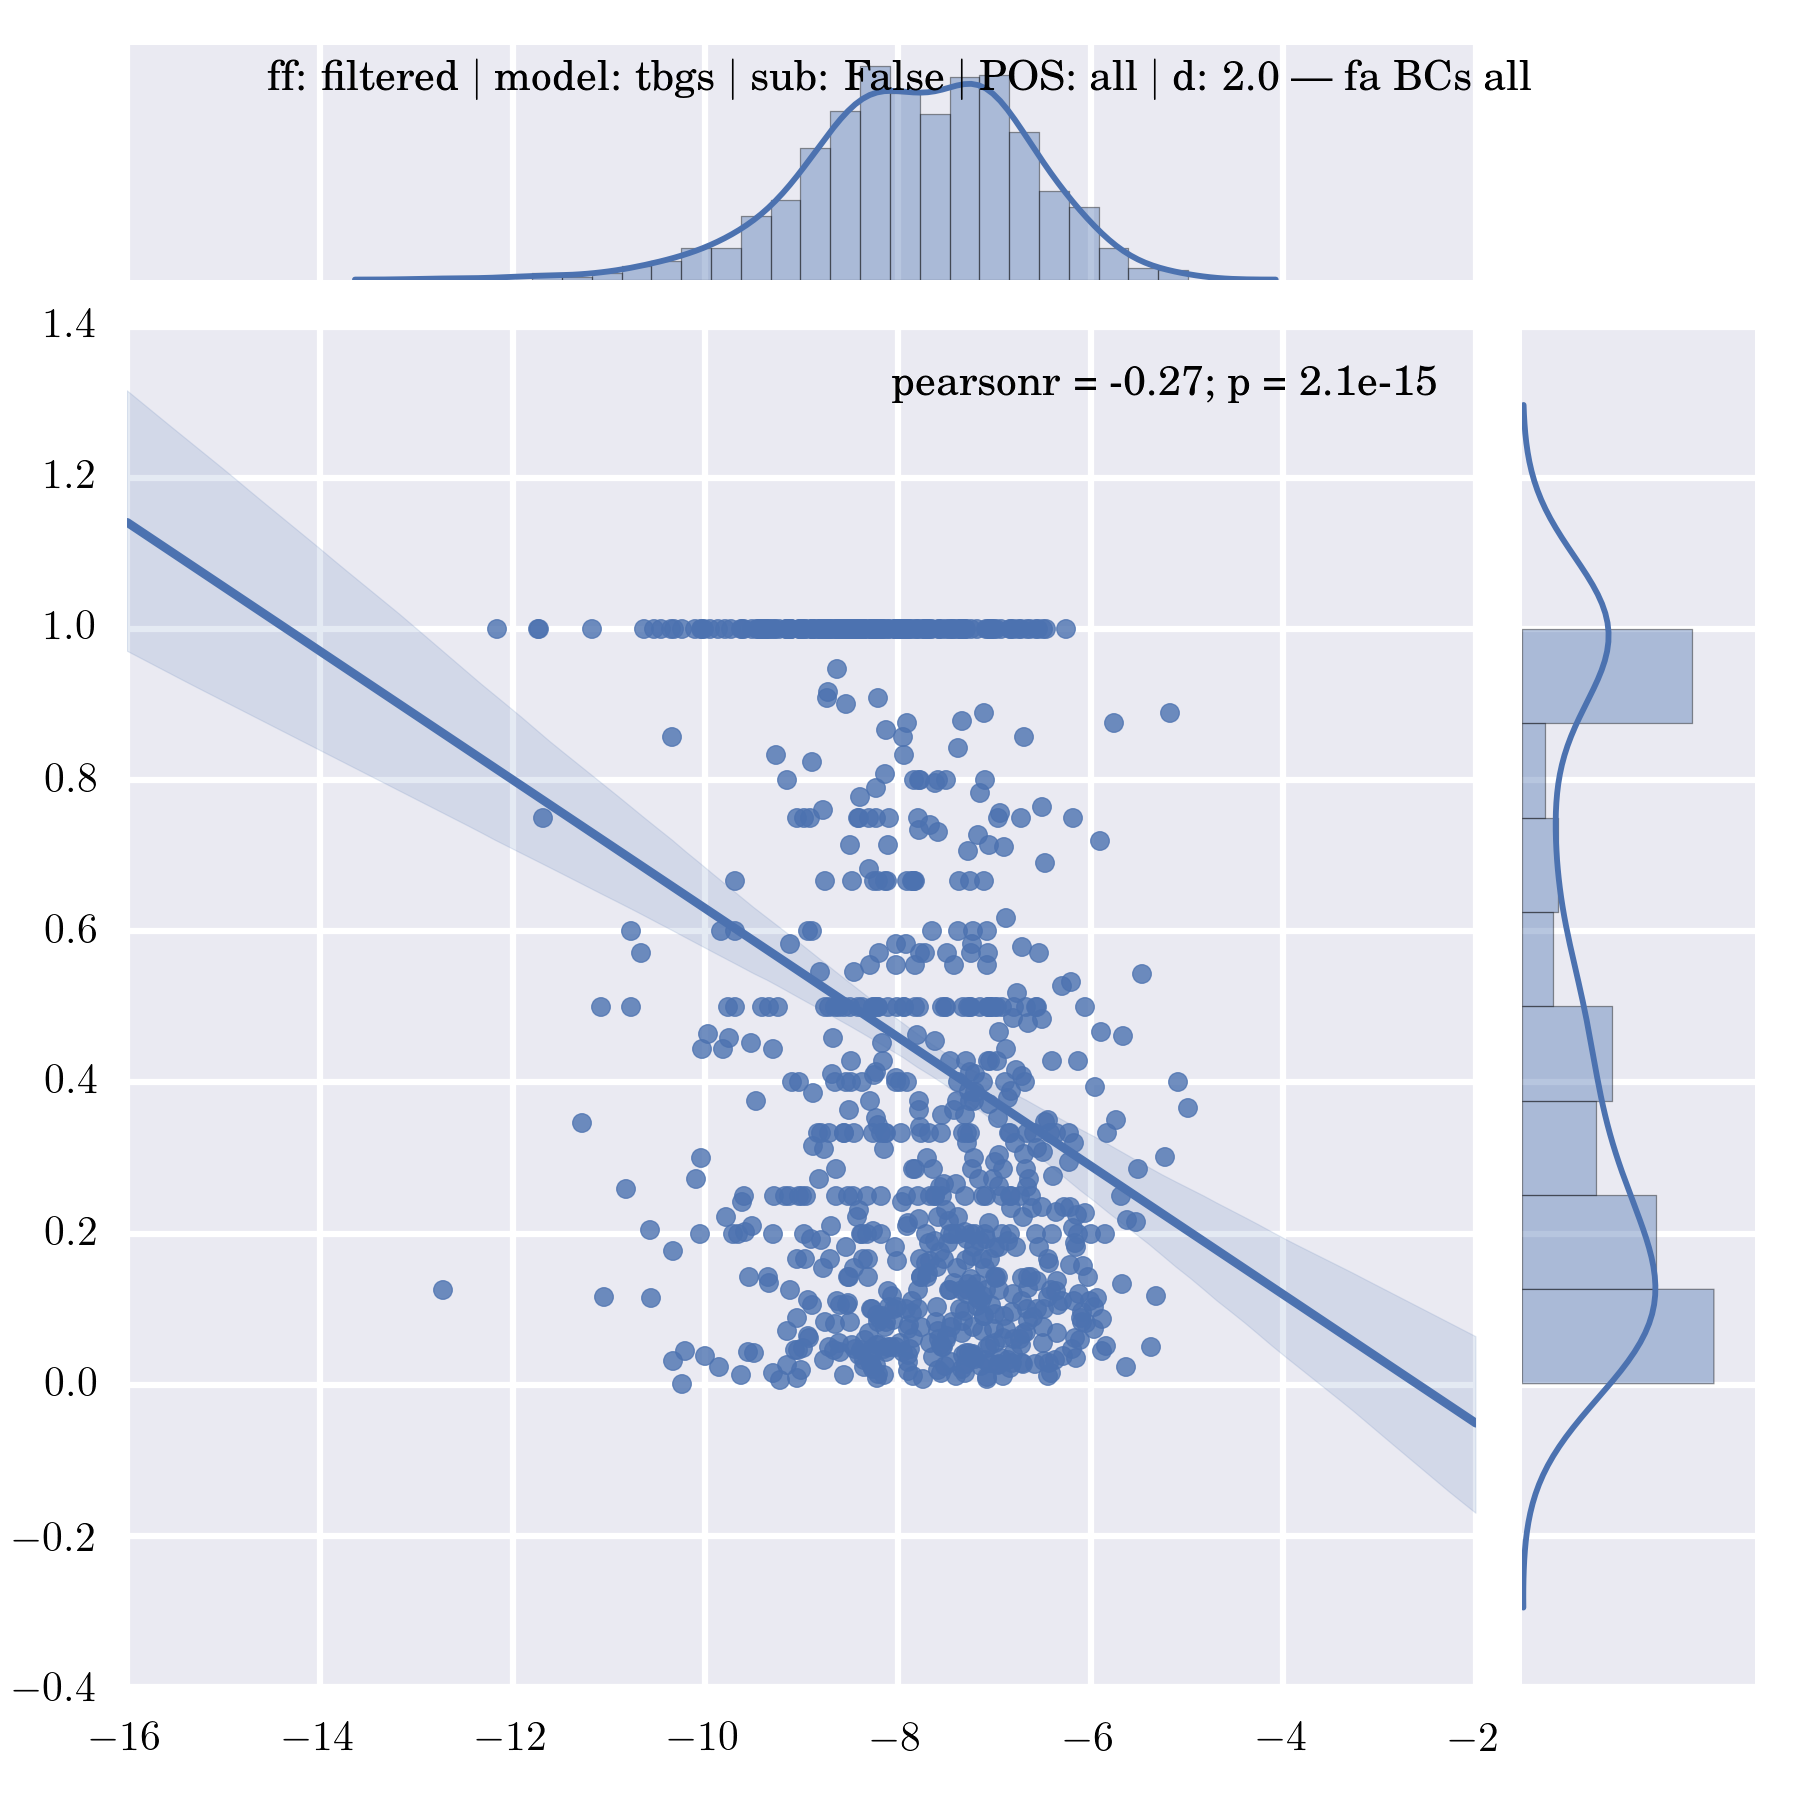
\includegraphics[width=0.3\textwidth]{images/feature-cards/fa_BCs/susceptibility_scatter.png}
	}
	~
	\subfloat[][Bin averages and KDE]{
		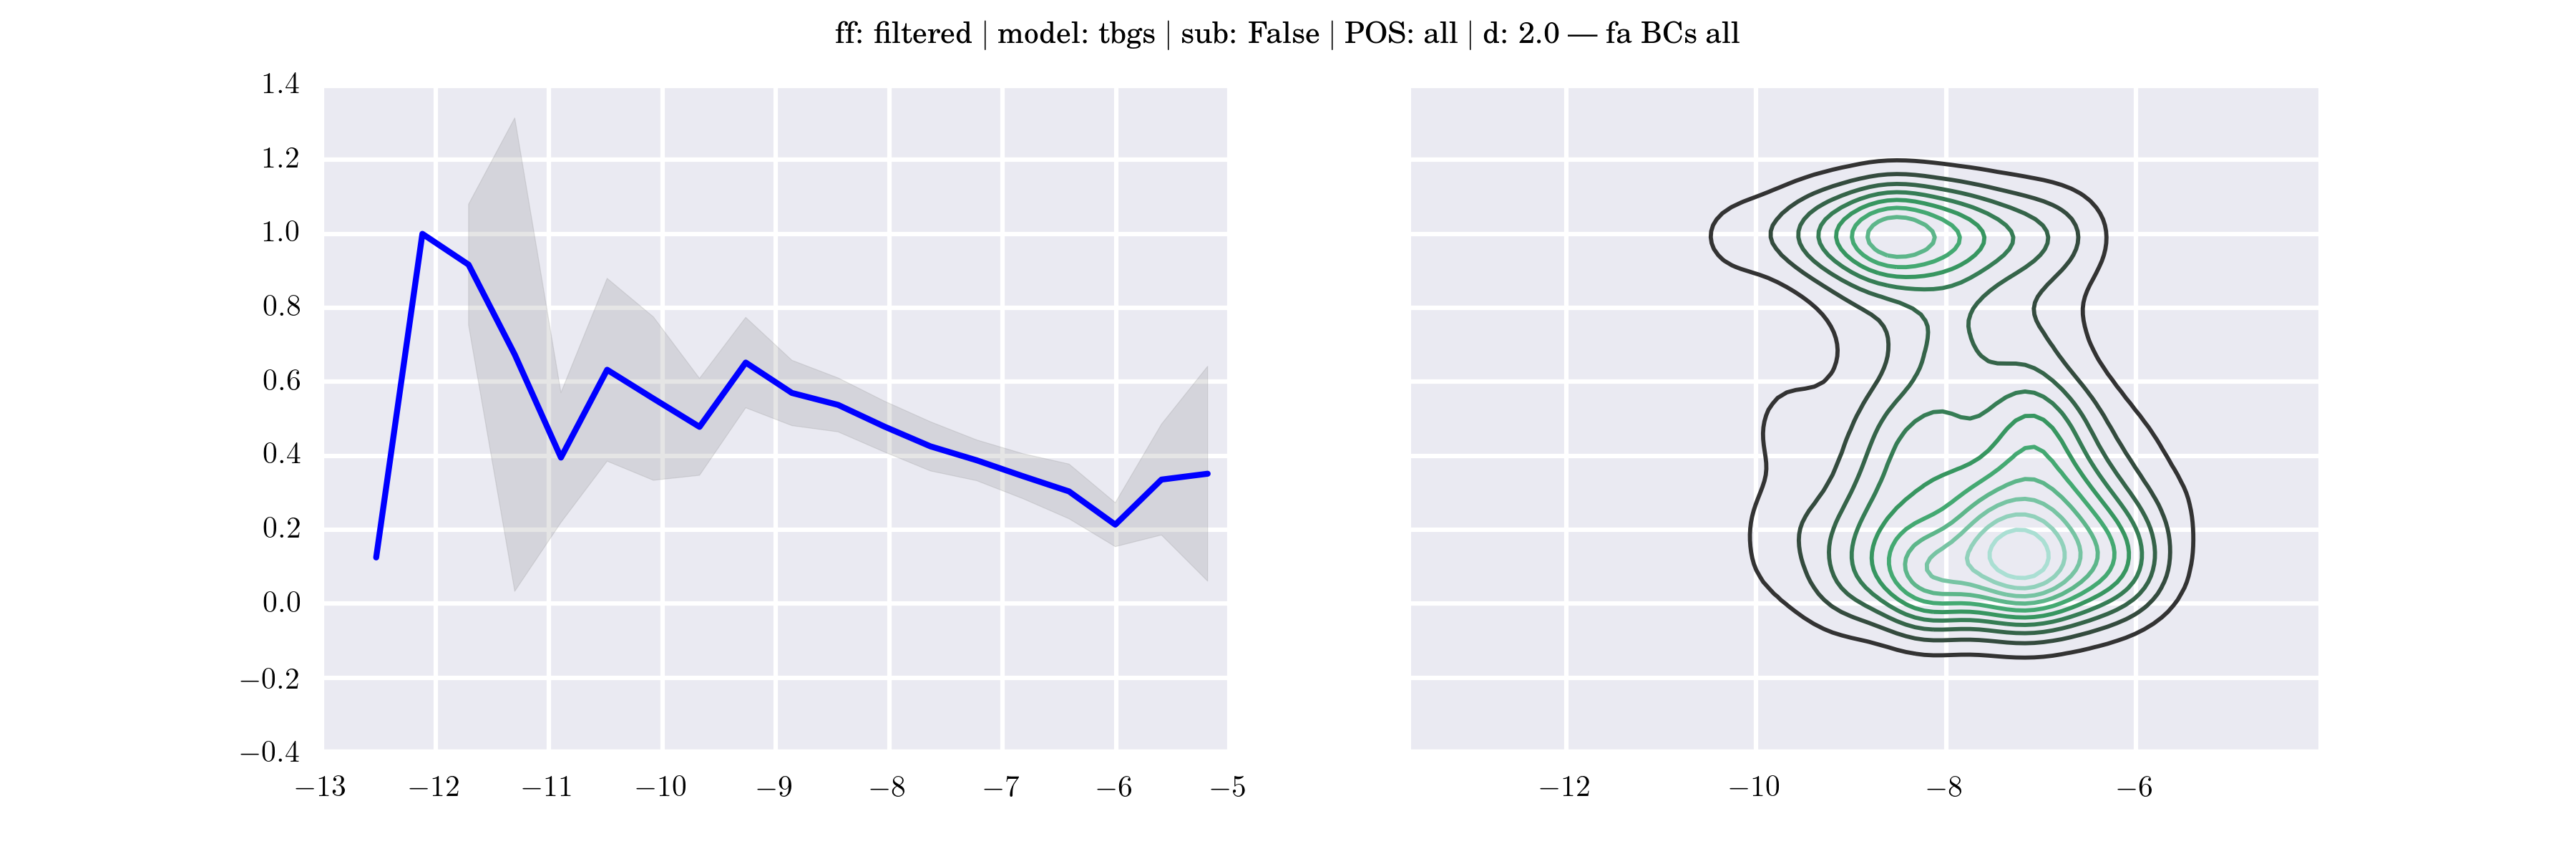
\includegraphics[width=0.6\textwidth]{images/feature-cards/fa_BCs/susceptibility.png}
	}
	\caption{Substitution susceptibility}
    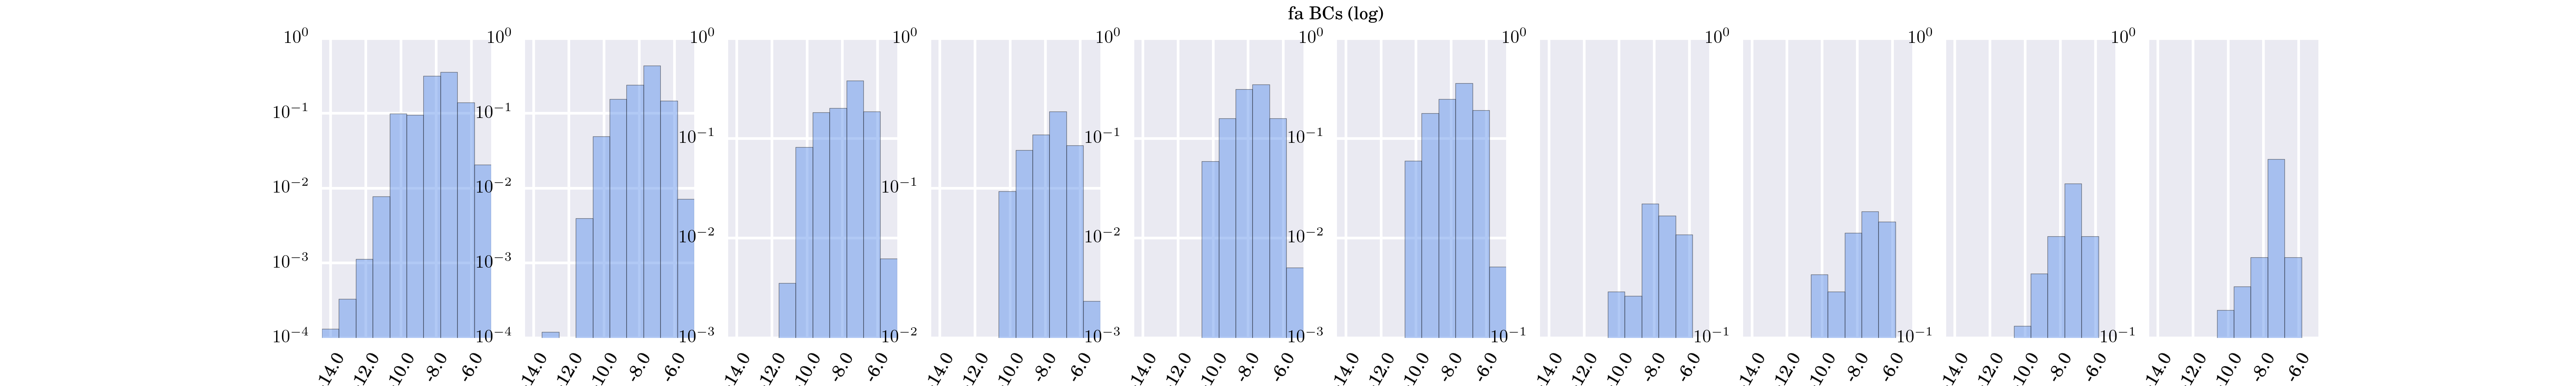
\includegraphics[width=\textwidth]{images/feature-cards/fa_BCs/timebags_evolution-hist.png}
	\caption{Timebag evolution}
\end{figure*}


% fa_CCs ===============================
\clearpage
\subsection{fa CCs}
\begin{figure*}[h!]
    \centering
    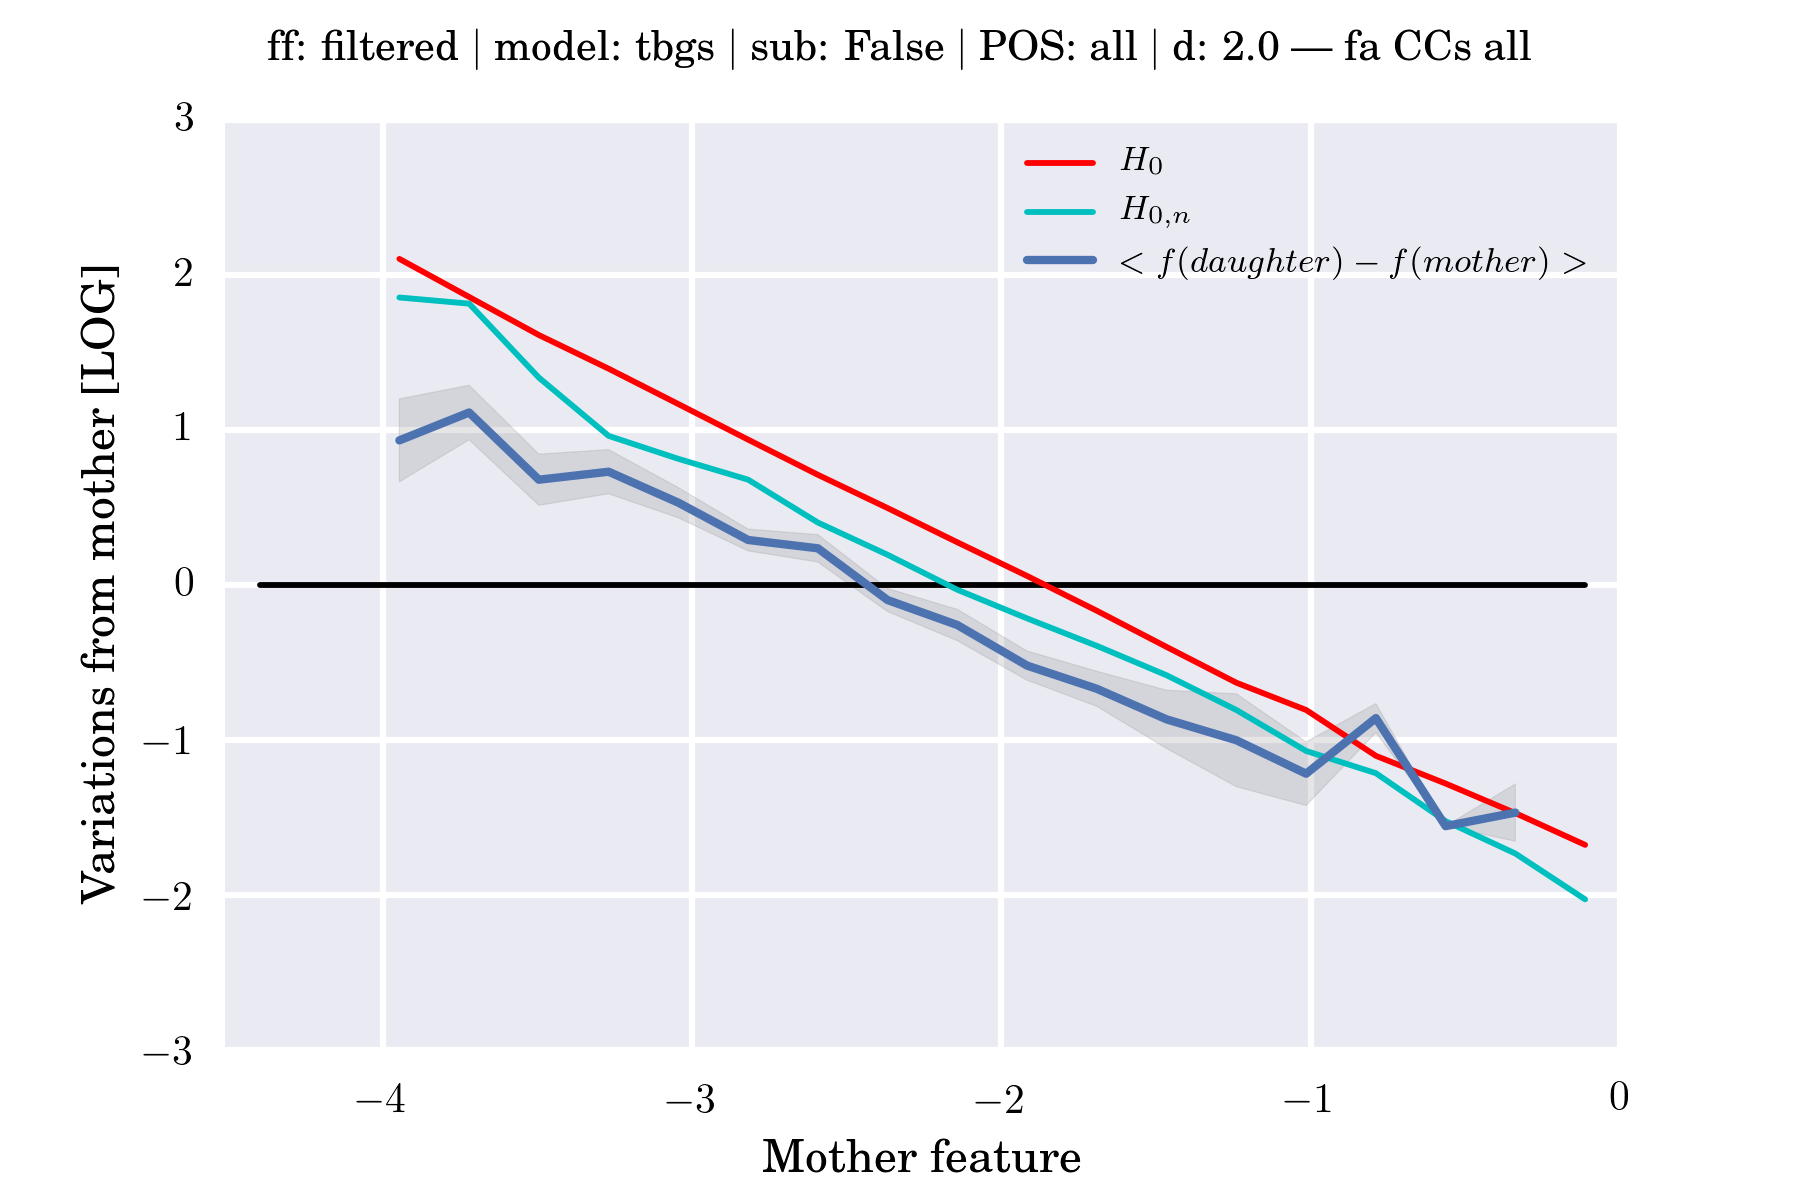
\includegraphics[width=0.6\textwidth]{images/feature-cards/fa_CCs/feature_variations.png}
    \caption{Feature variation on substitution}
	\subfloat[][Scatter plot]{
		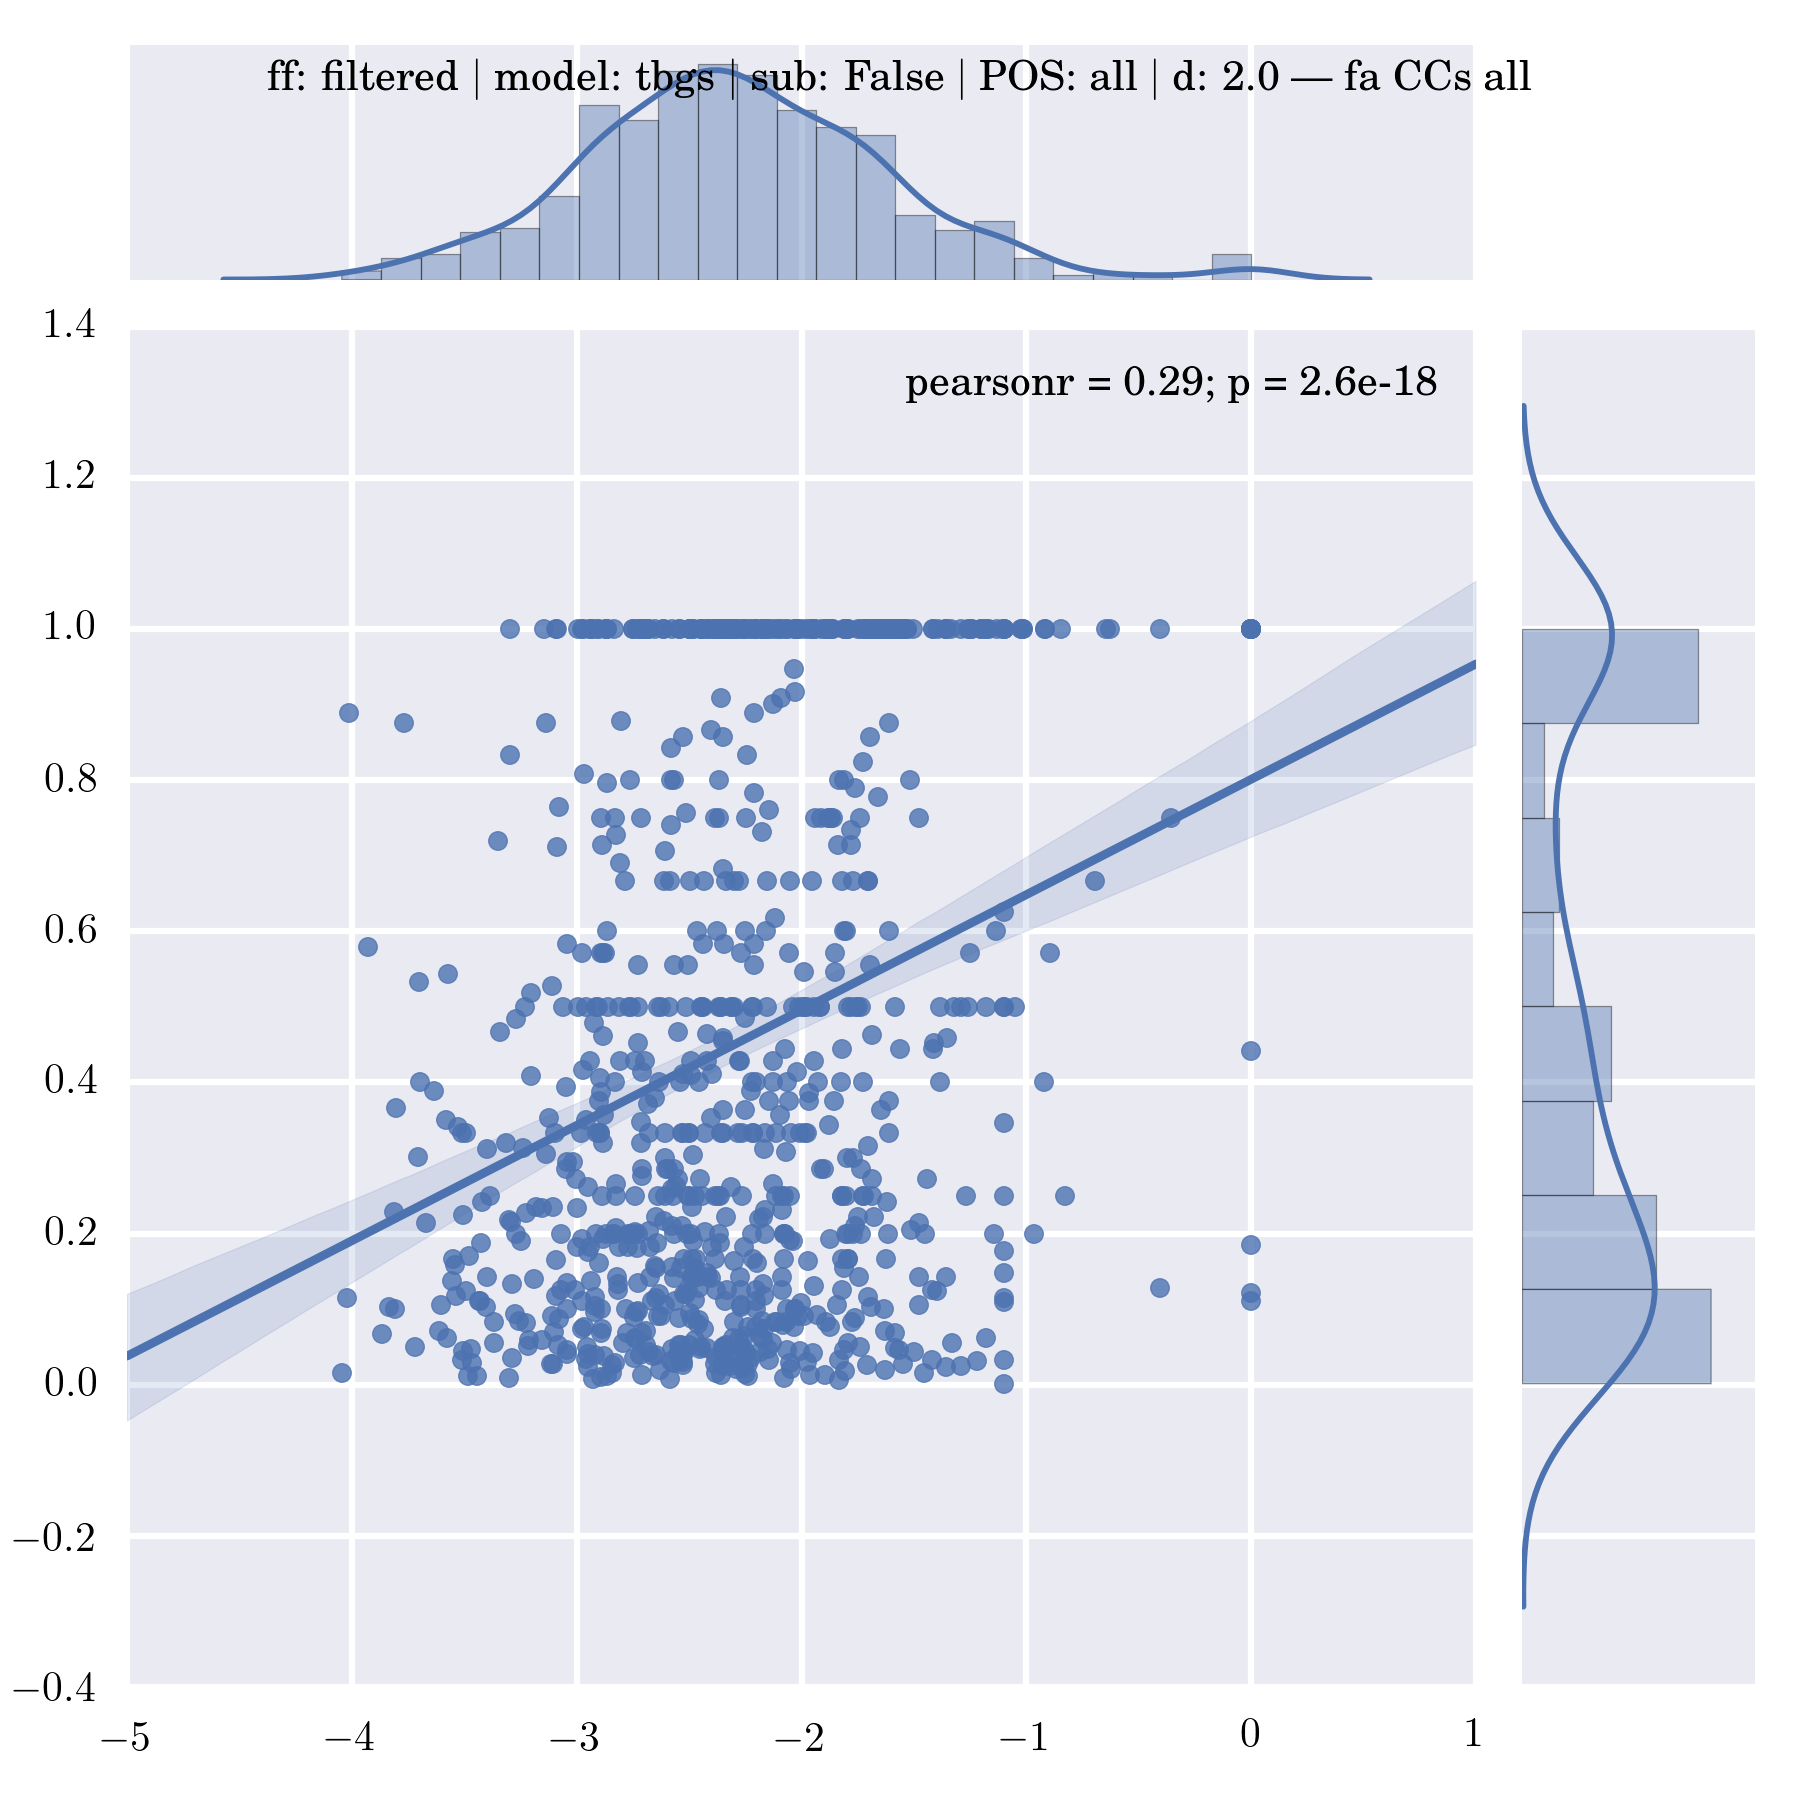
\includegraphics[width=0.3\textwidth]{images/feature-cards/fa_CCs/susceptibility_scatter.png}
	}
	~
	\subfloat[][Bin averages and KDE]{
		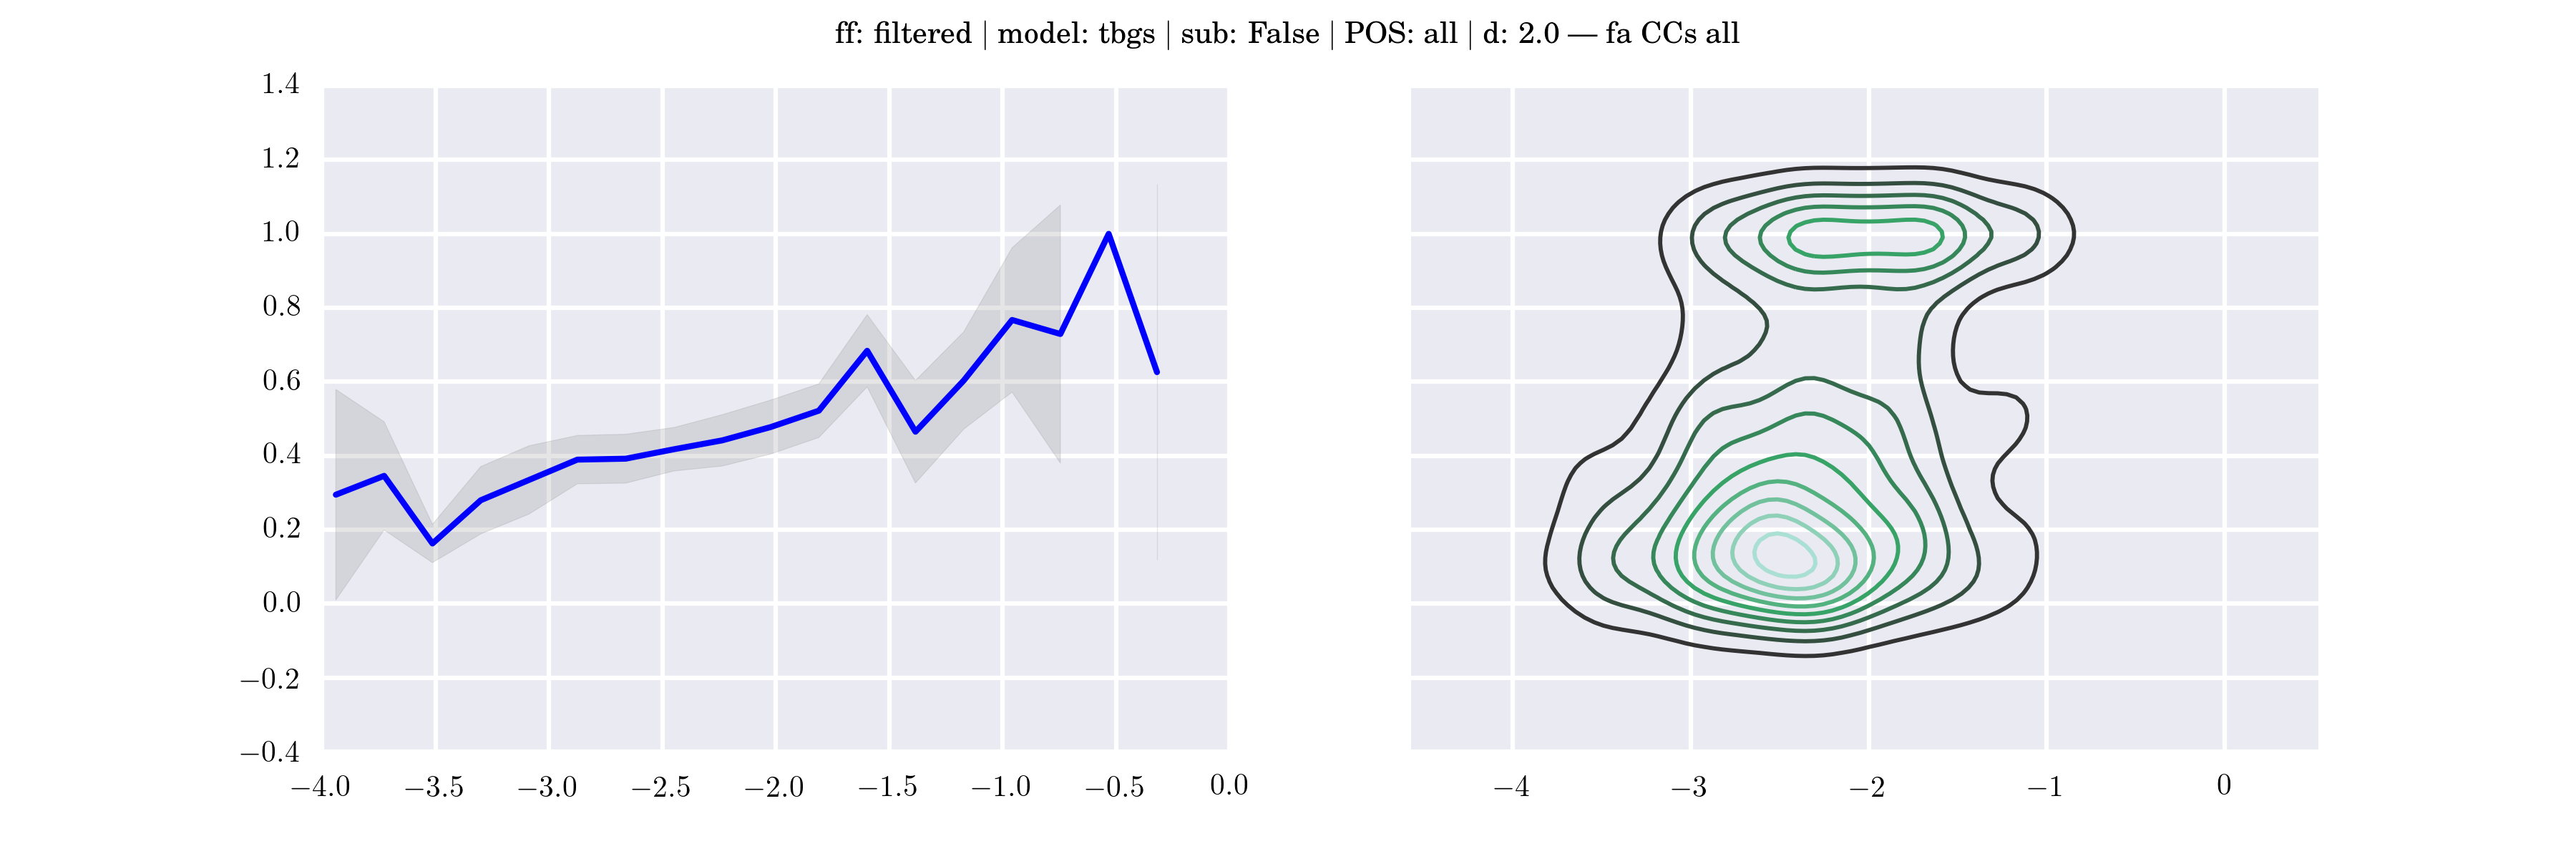
\includegraphics[width=0.6\textwidth]{images/feature-cards/fa_CCs/susceptibility.png}
	}
	\caption{Substitution susceptibility}
    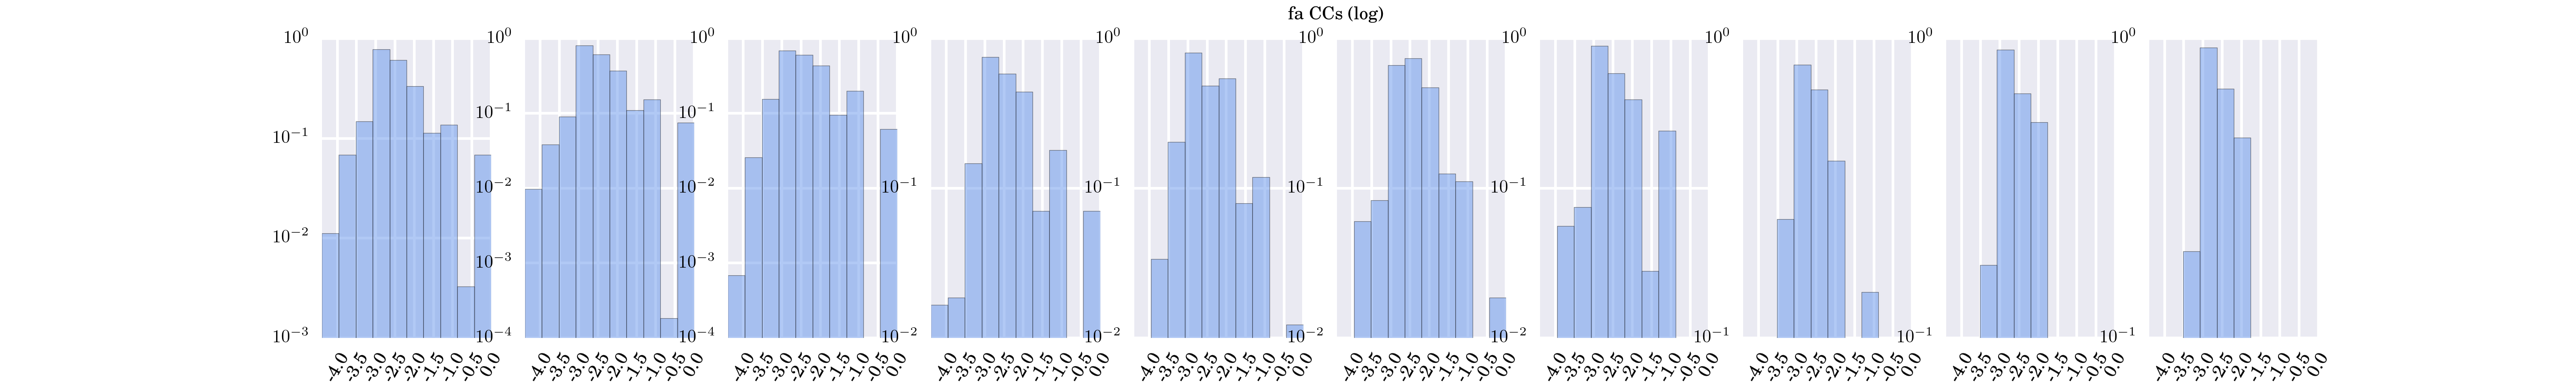
\includegraphics[width=\textwidth]{images/feature-cards/fa_CCs/timebags_evolution-hist.png}
	\caption{Timebag evolution}
\end{figure*}


% fa_degrees ===============================
\clearpage
\subsection{fa degrees}
\begin{figure*}[h!]
    \centering
    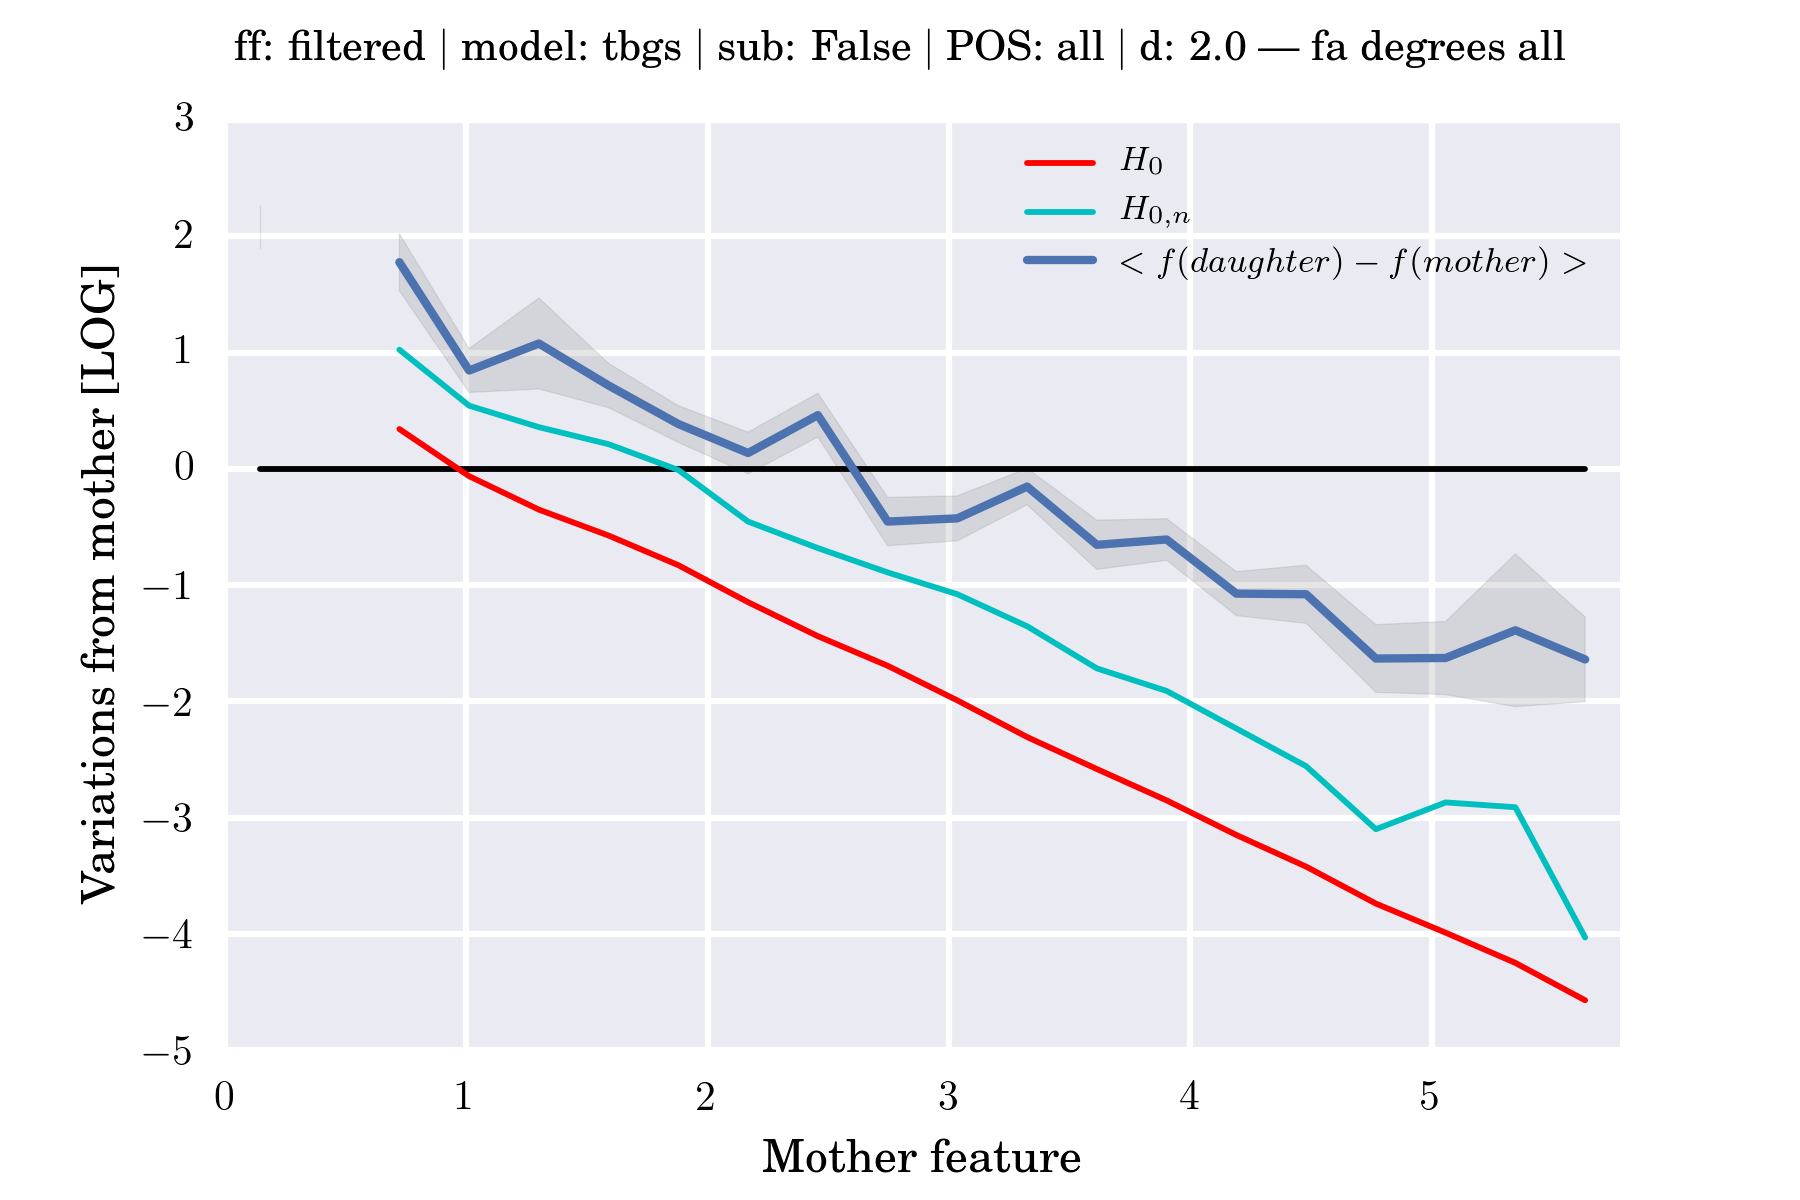
\includegraphics[width=0.6\textwidth]{images/feature-cards/fa_degrees/feature_variations.png}
    \caption{Feature variation on substitution}
	\subfloat[][Scatter plot]{
		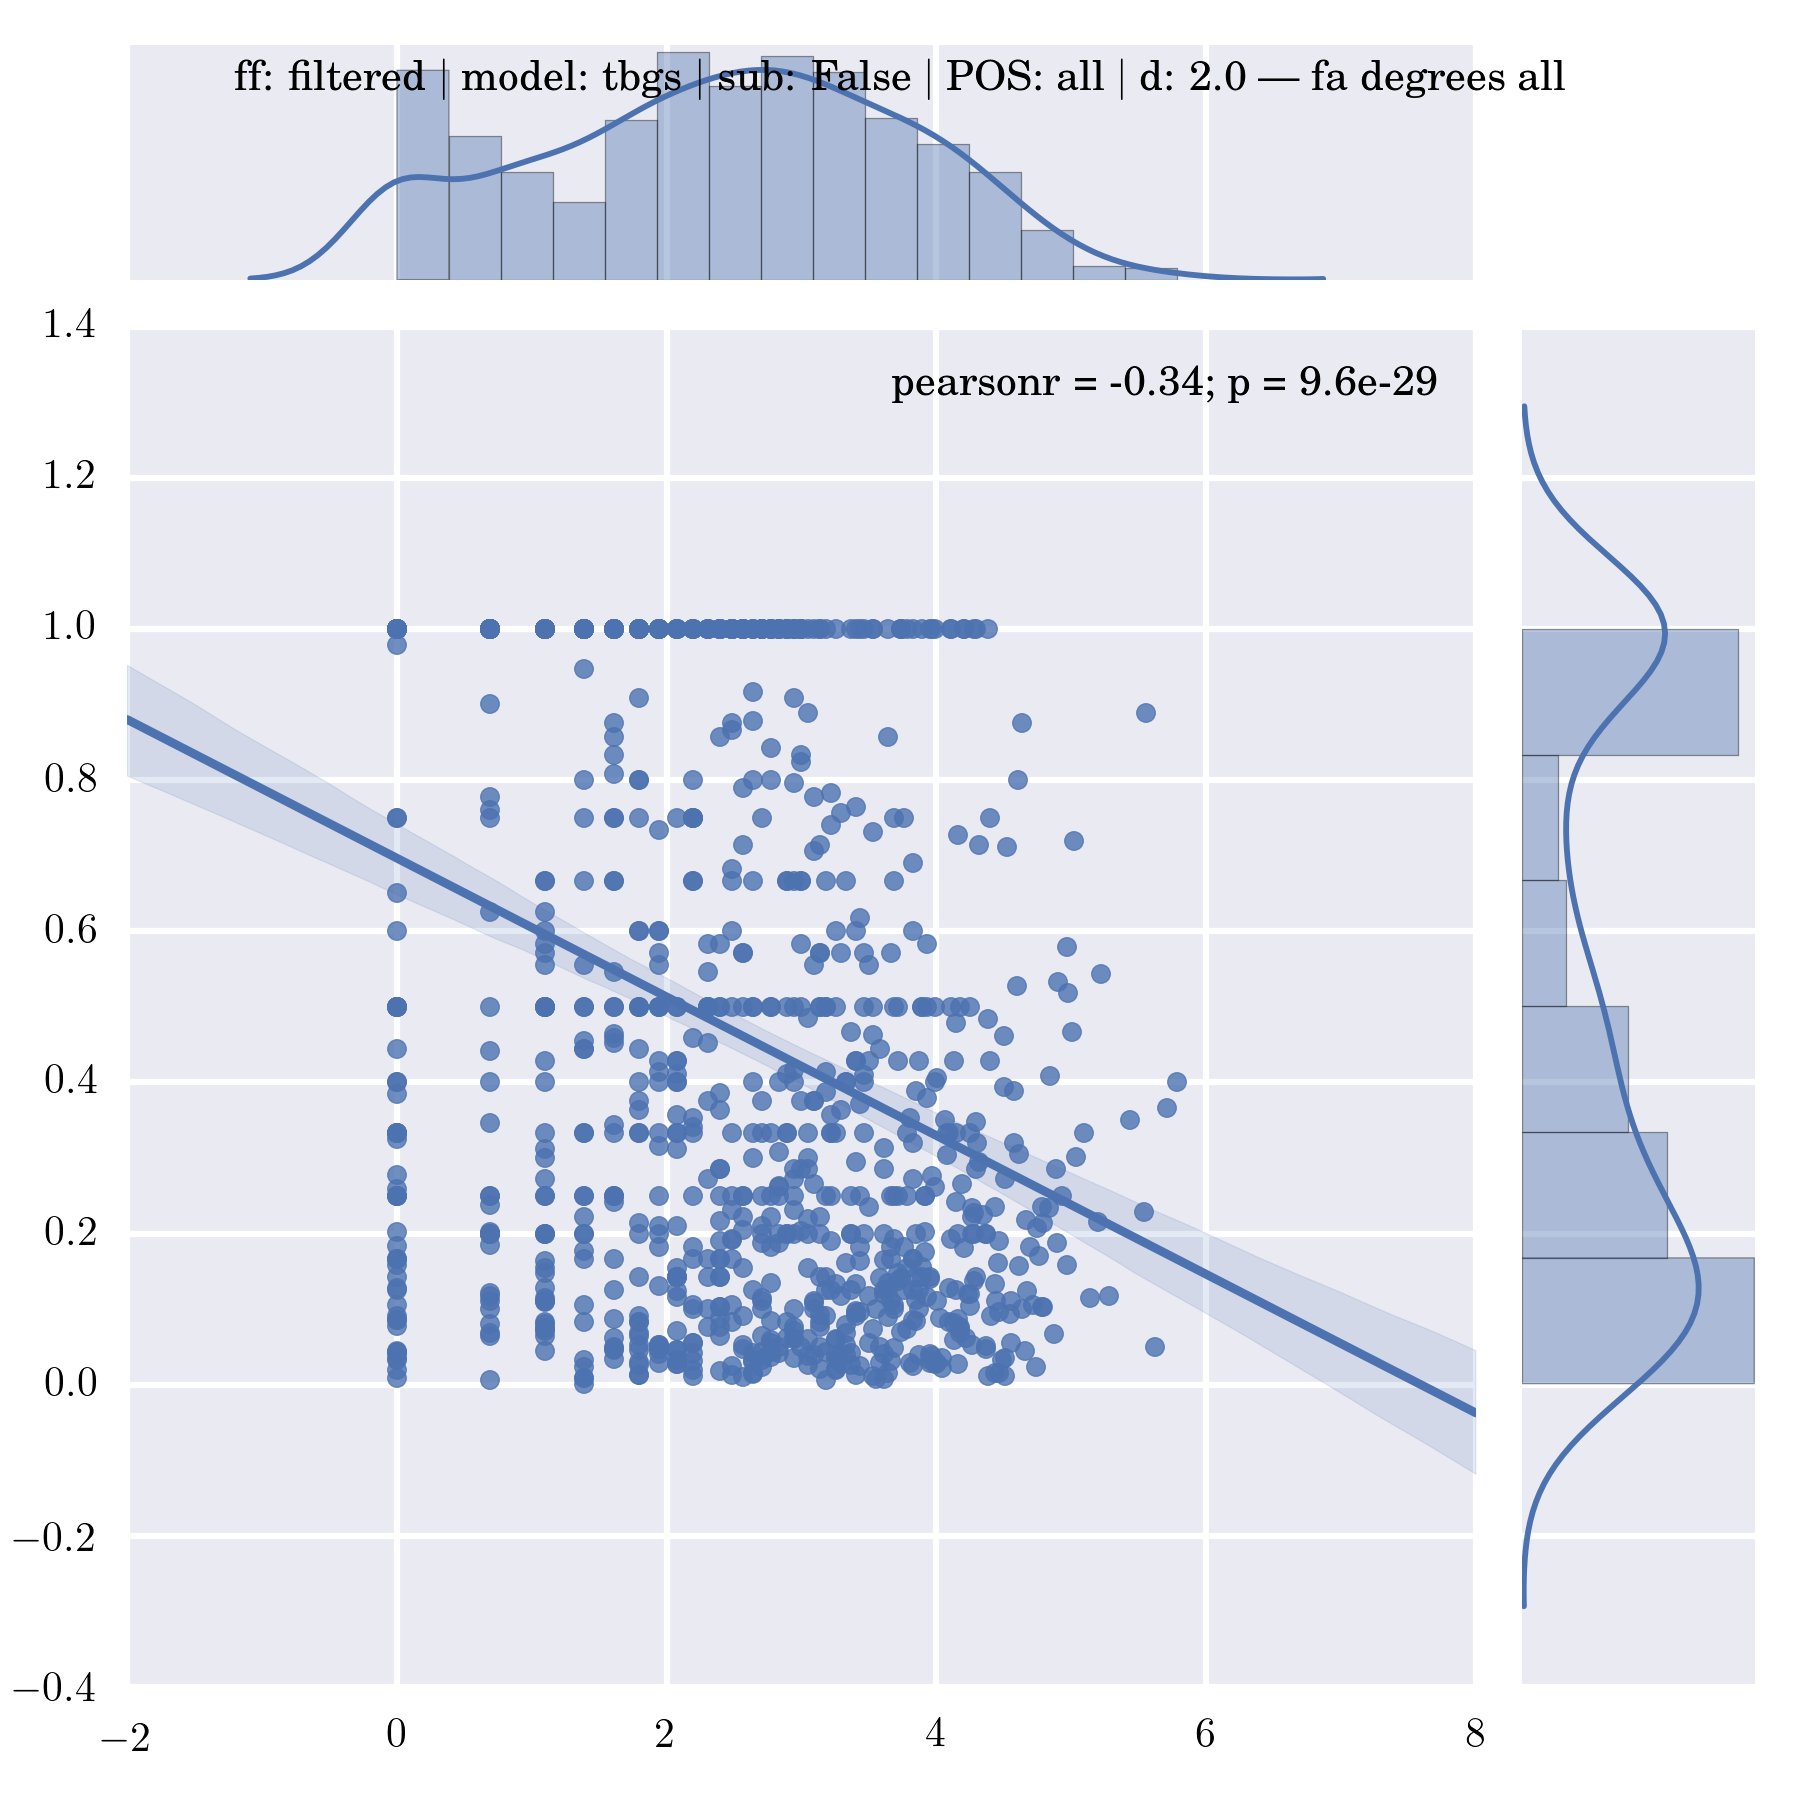
\includegraphics[width=0.3\textwidth]{images/feature-cards/fa_degrees/susceptibility_scatter.png}
	}
	~
	\subfloat[][Bin averages and KDE]{
		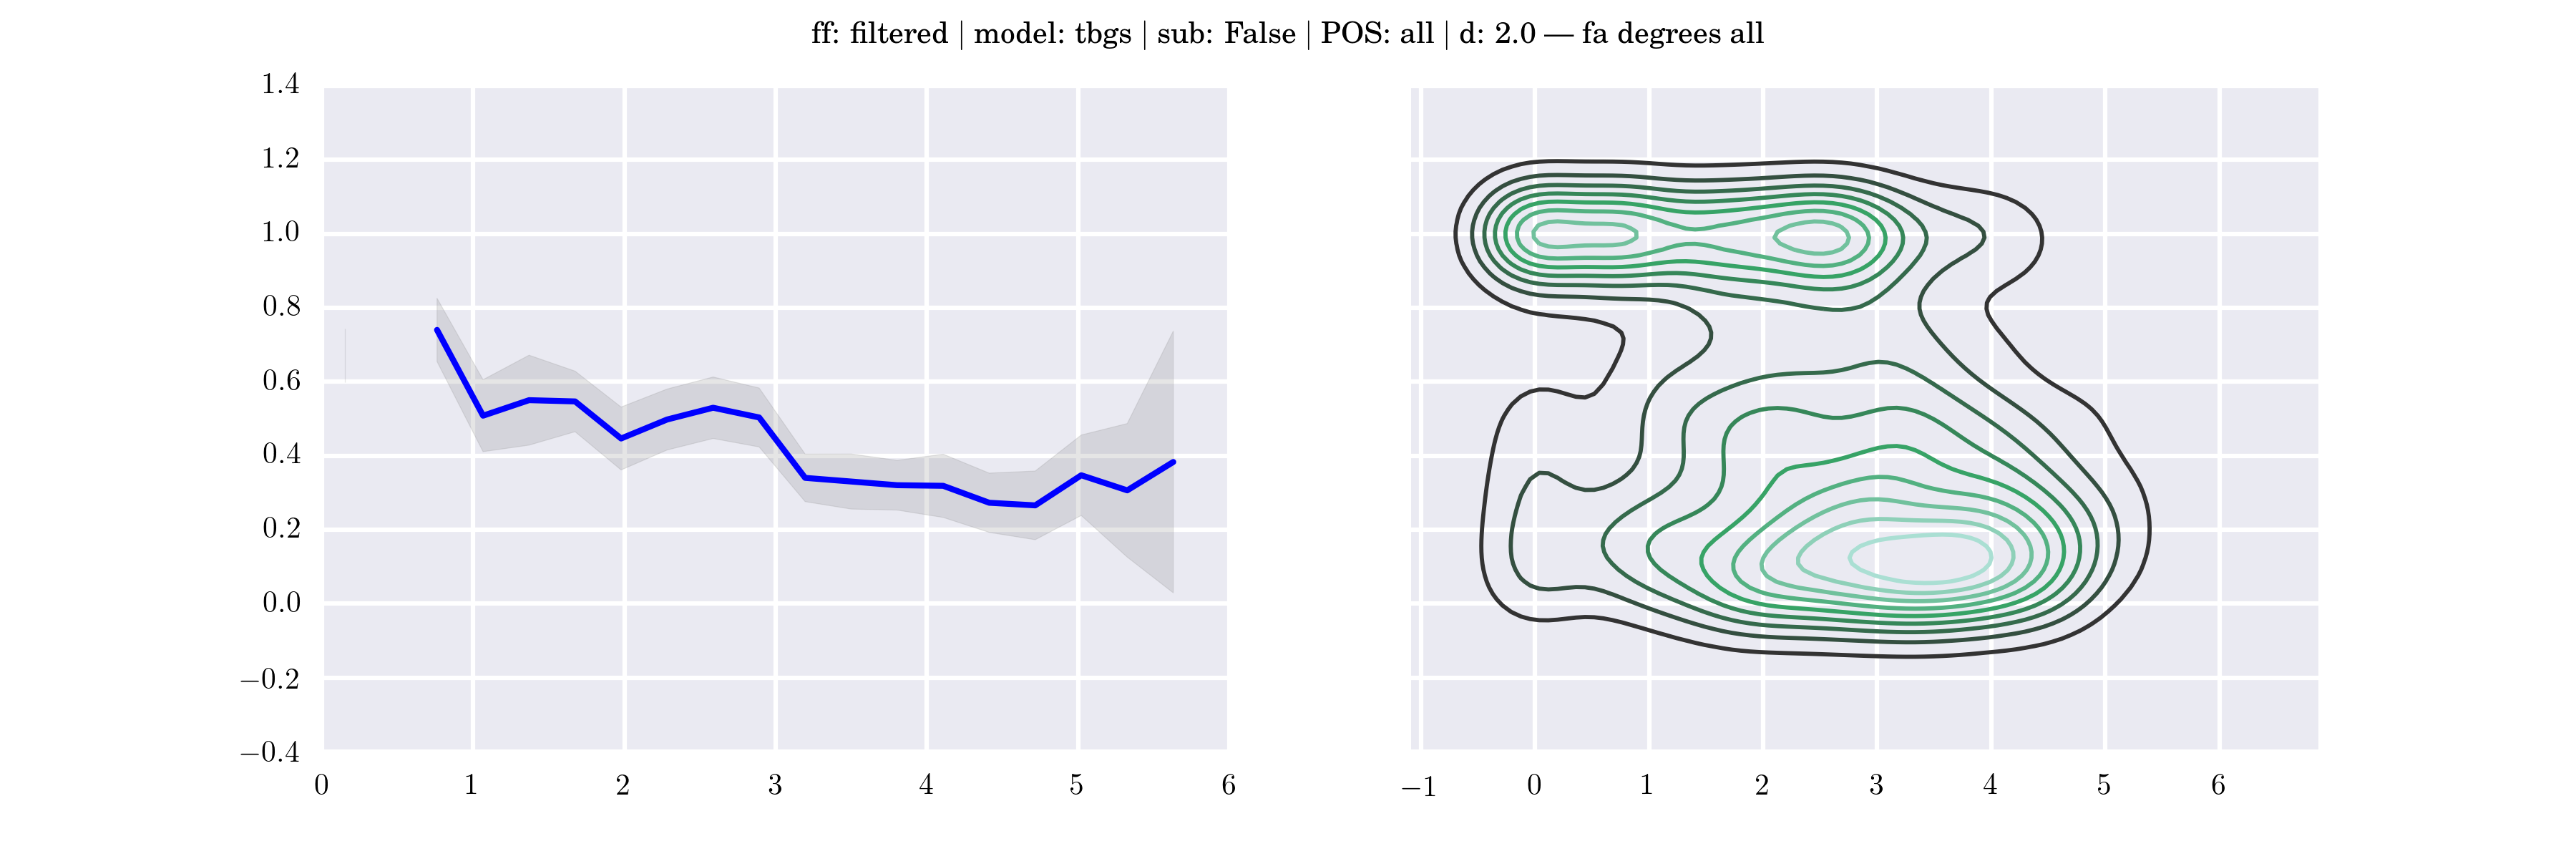
\includegraphics[width=0.6\textwidth]{images/feature-cards/fa_degrees/susceptibility.png}
	}
	\caption{Substitution susceptibility}
    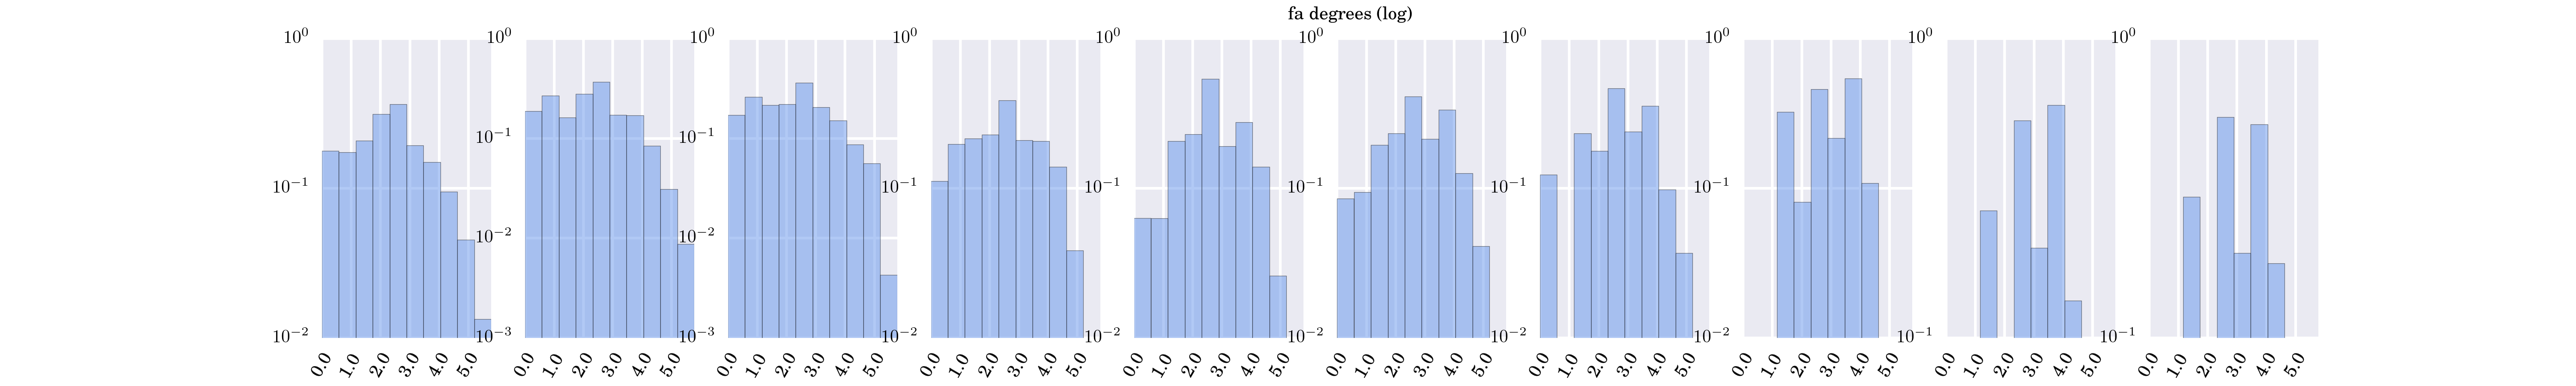
\includegraphics[width=\textwidth]{images/feature-cards/fa_degrees/timebags_evolution-hist.png}
	\caption{Timebag evolution}
\end{figure*}


% fa_PR_scores ===============================
\clearpage
\subsection{fa PR scores}
\begin{figure*}[h!]
    \centering
    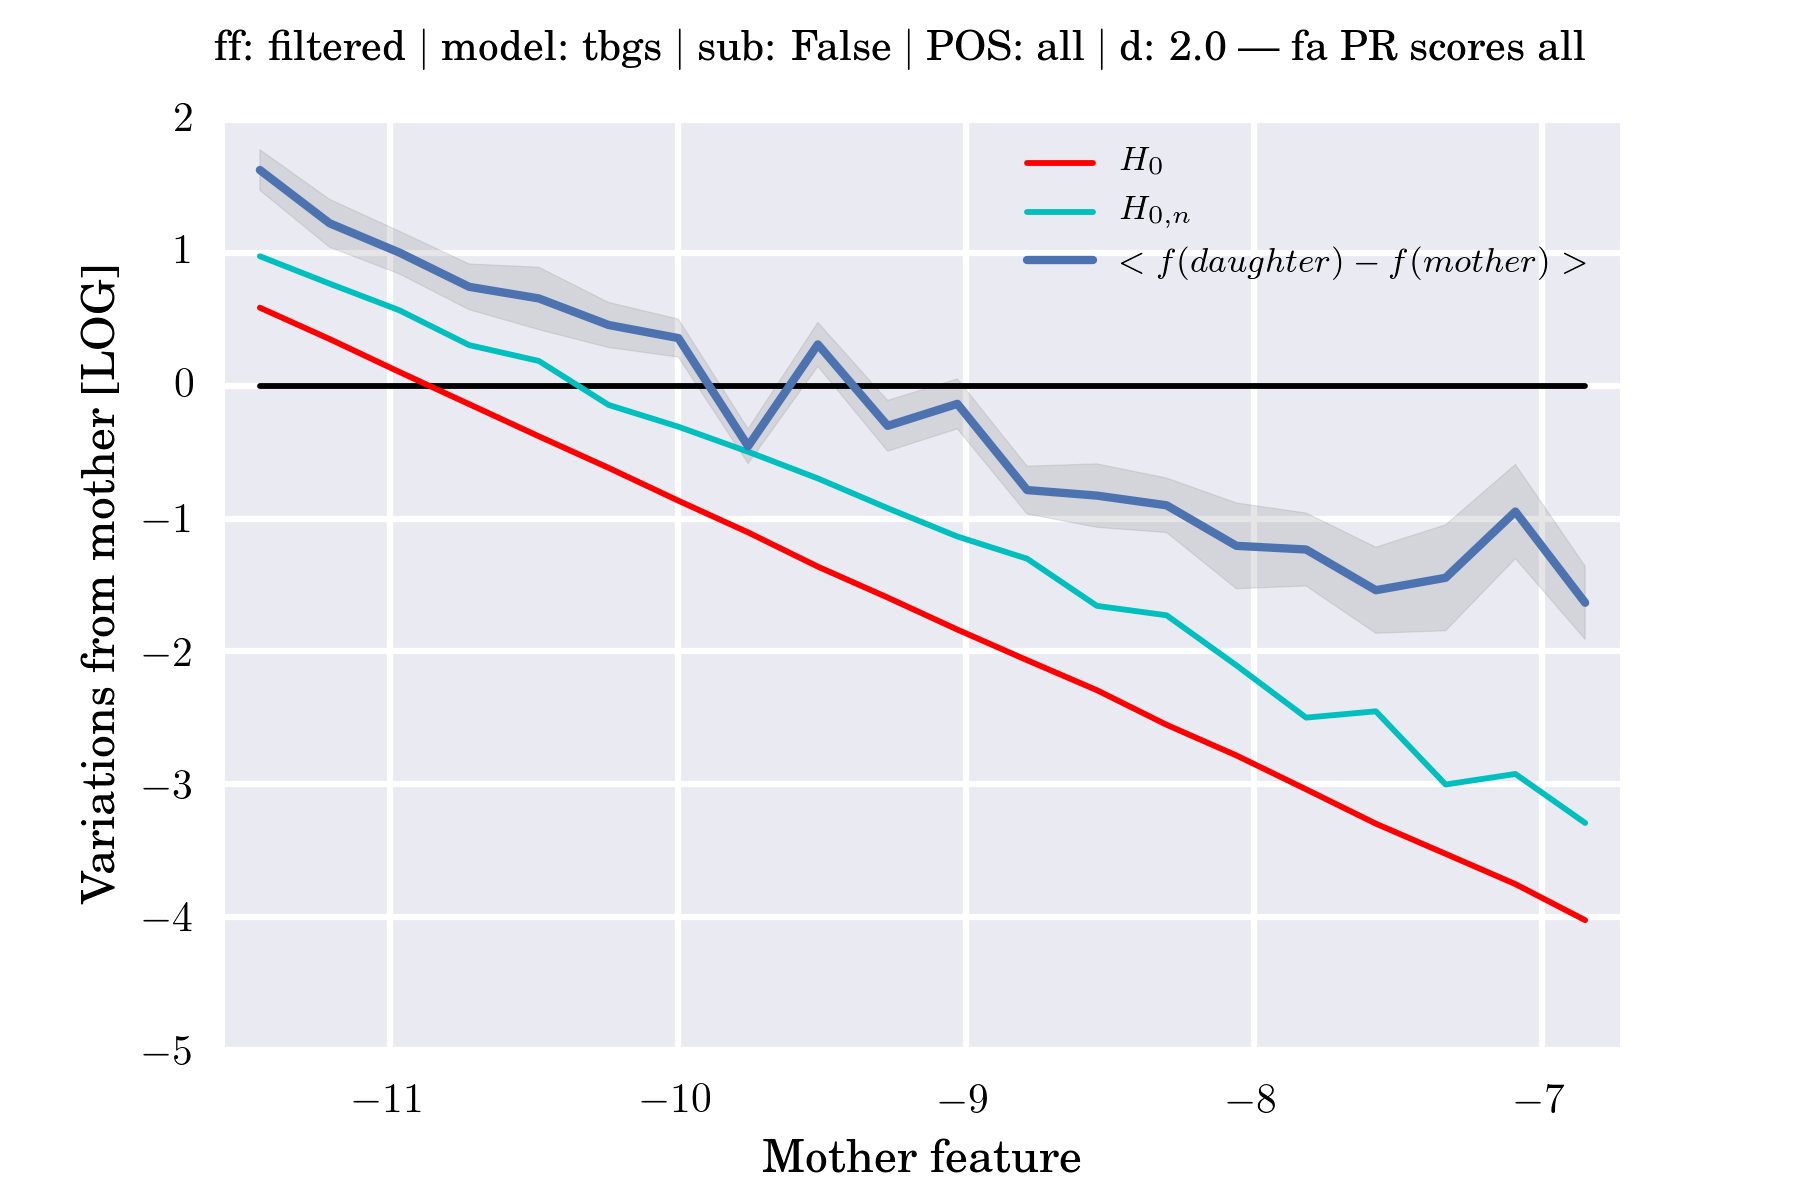
\includegraphics[width=0.6\textwidth]{images/feature-cards/fa_PR_scores/feature_variations.png}
    \caption{Feature variation on substitution}
	\subfloat[][Scatter plot]{
		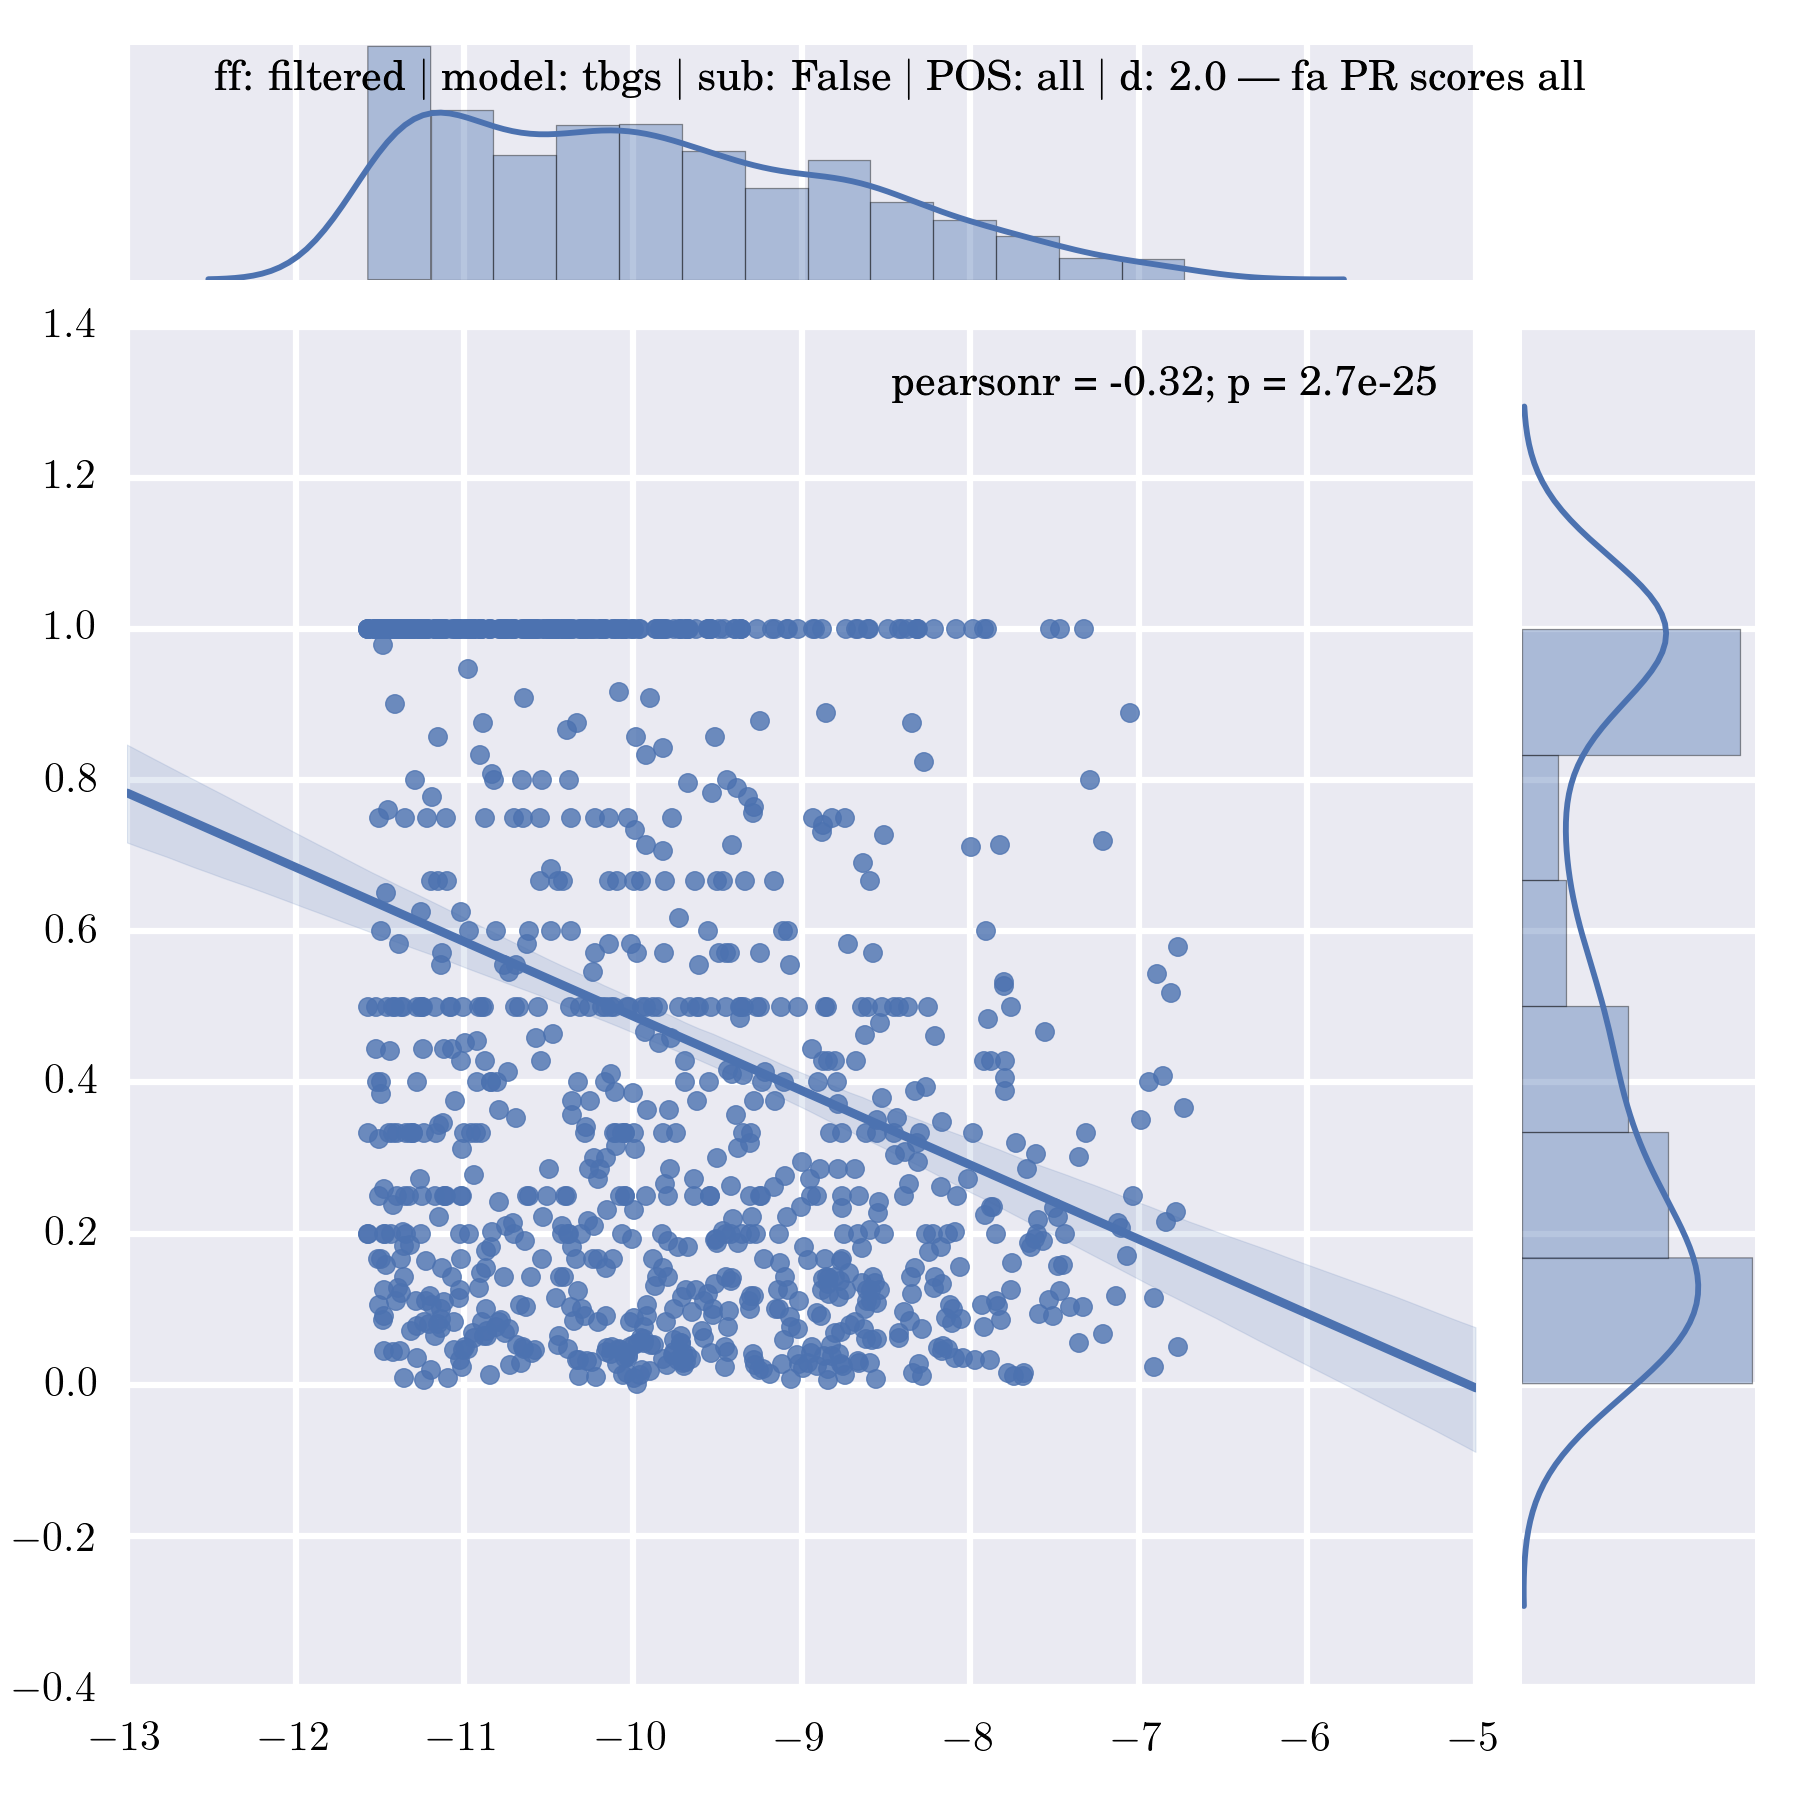
\includegraphics[width=0.3\textwidth]{images/feature-cards/fa_PR_scores/susceptibility_scatter.png}
	}
	~
	\subfloat[][Bin averages and KDE]{
		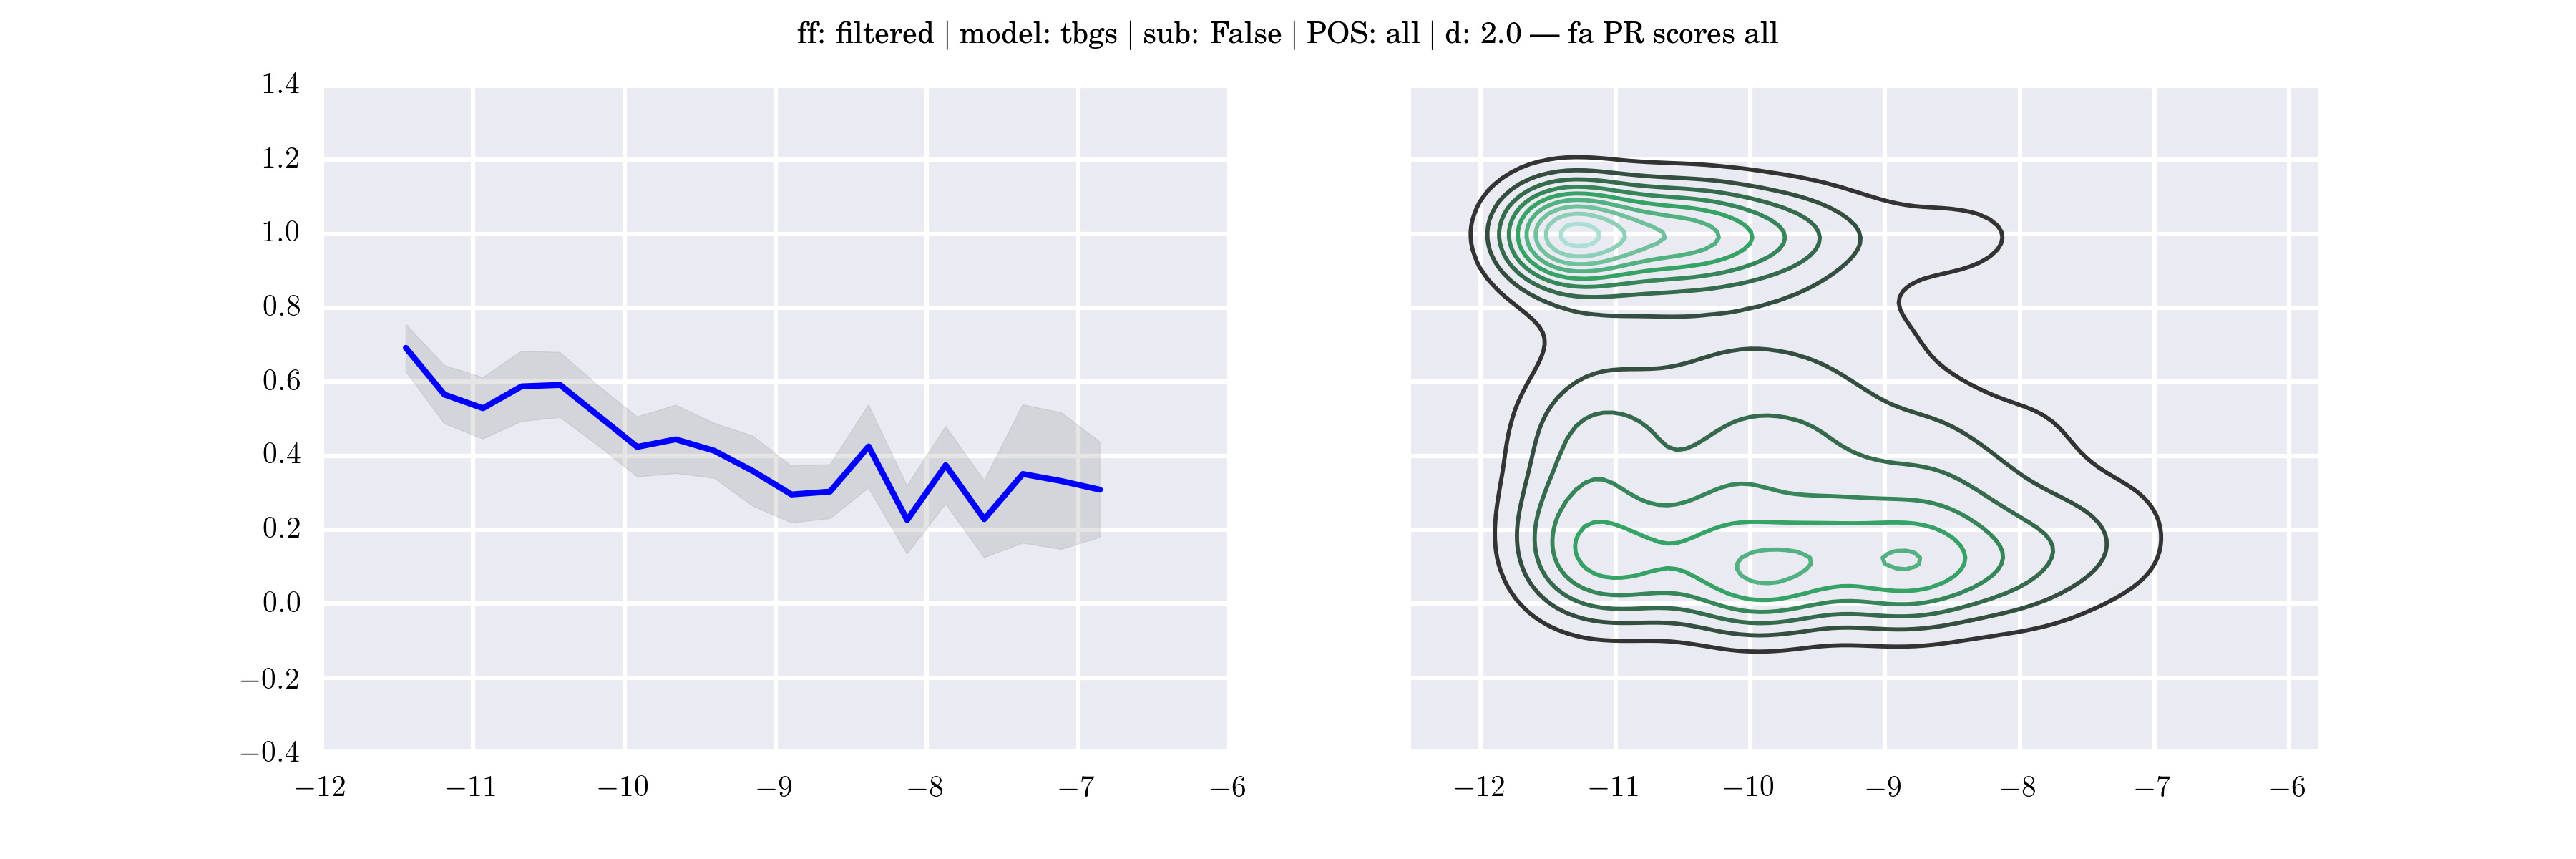
\includegraphics[width=0.6\textwidth]{images/feature-cards/fa_PR_scores/susceptibility.png}
	}
	\caption{Substitution susceptibility}
    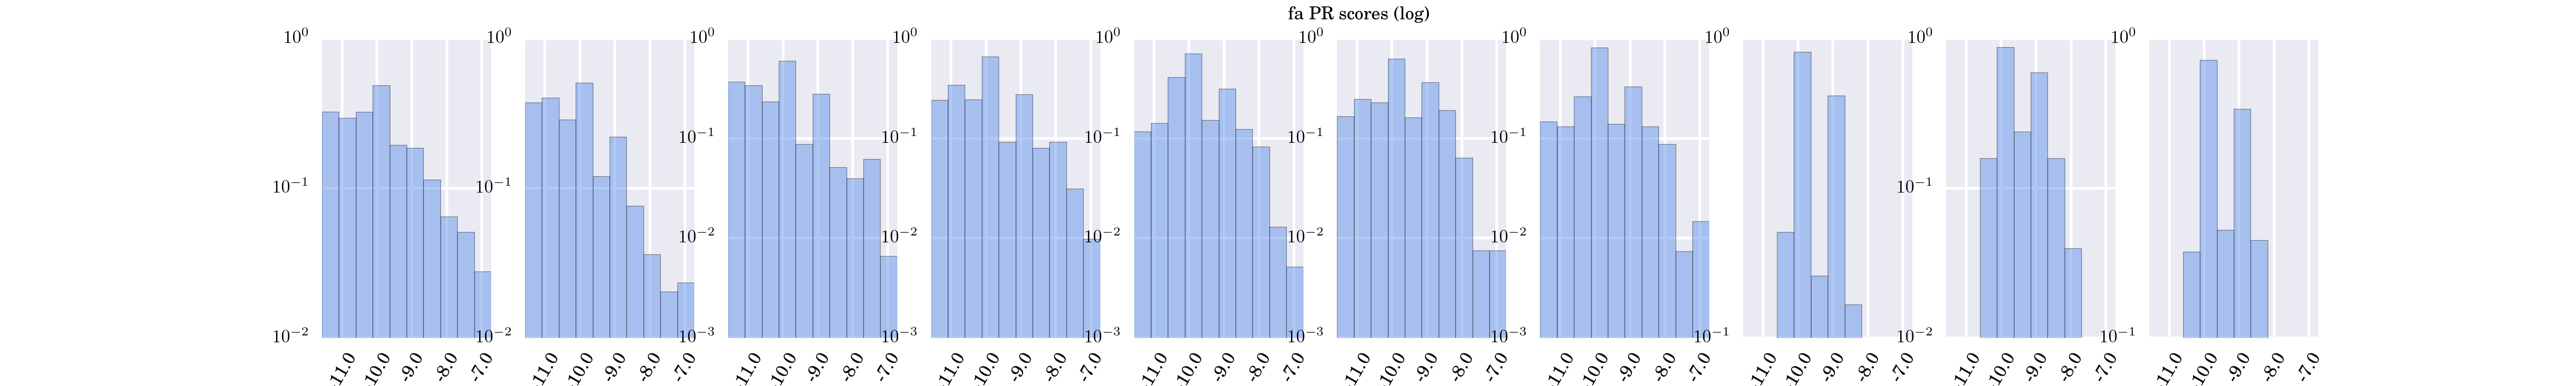
\includegraphics[width=\textwidth]{images/feature-cards/fa_PR_scores/timebags_evolution-hist.png}
	\caption{Timebag evolution}
\end{figure*}


% mt_frequencies ===============================
\clearpage
\subsection{mt frequencies}
\begin{figure*}[h!]
    \centering
    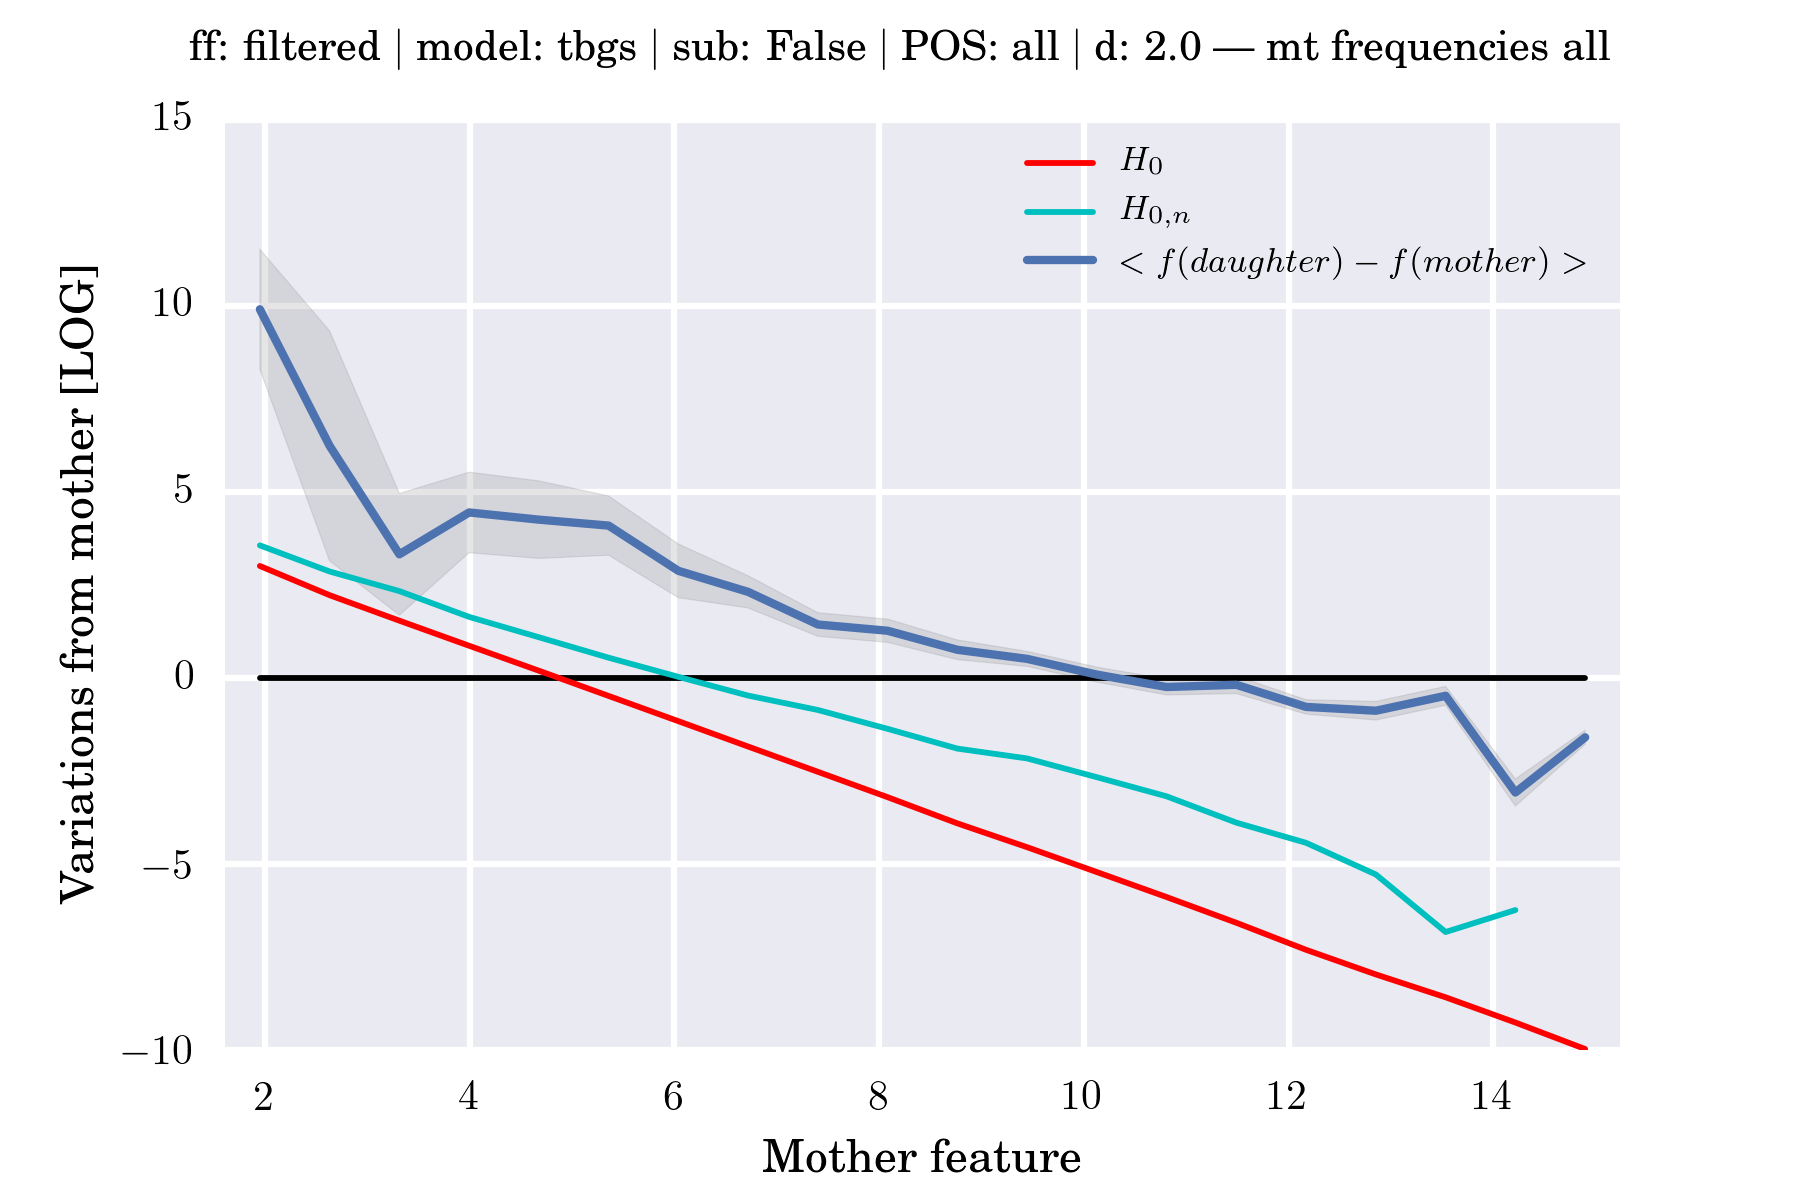
\includegraphics[width=0.6\textwidth]{images/feature-cards/mt_frequencies/feature_variations.png}
    \caption{Feature variation on substitution}
	\subfloat[][Scatter plot]{
		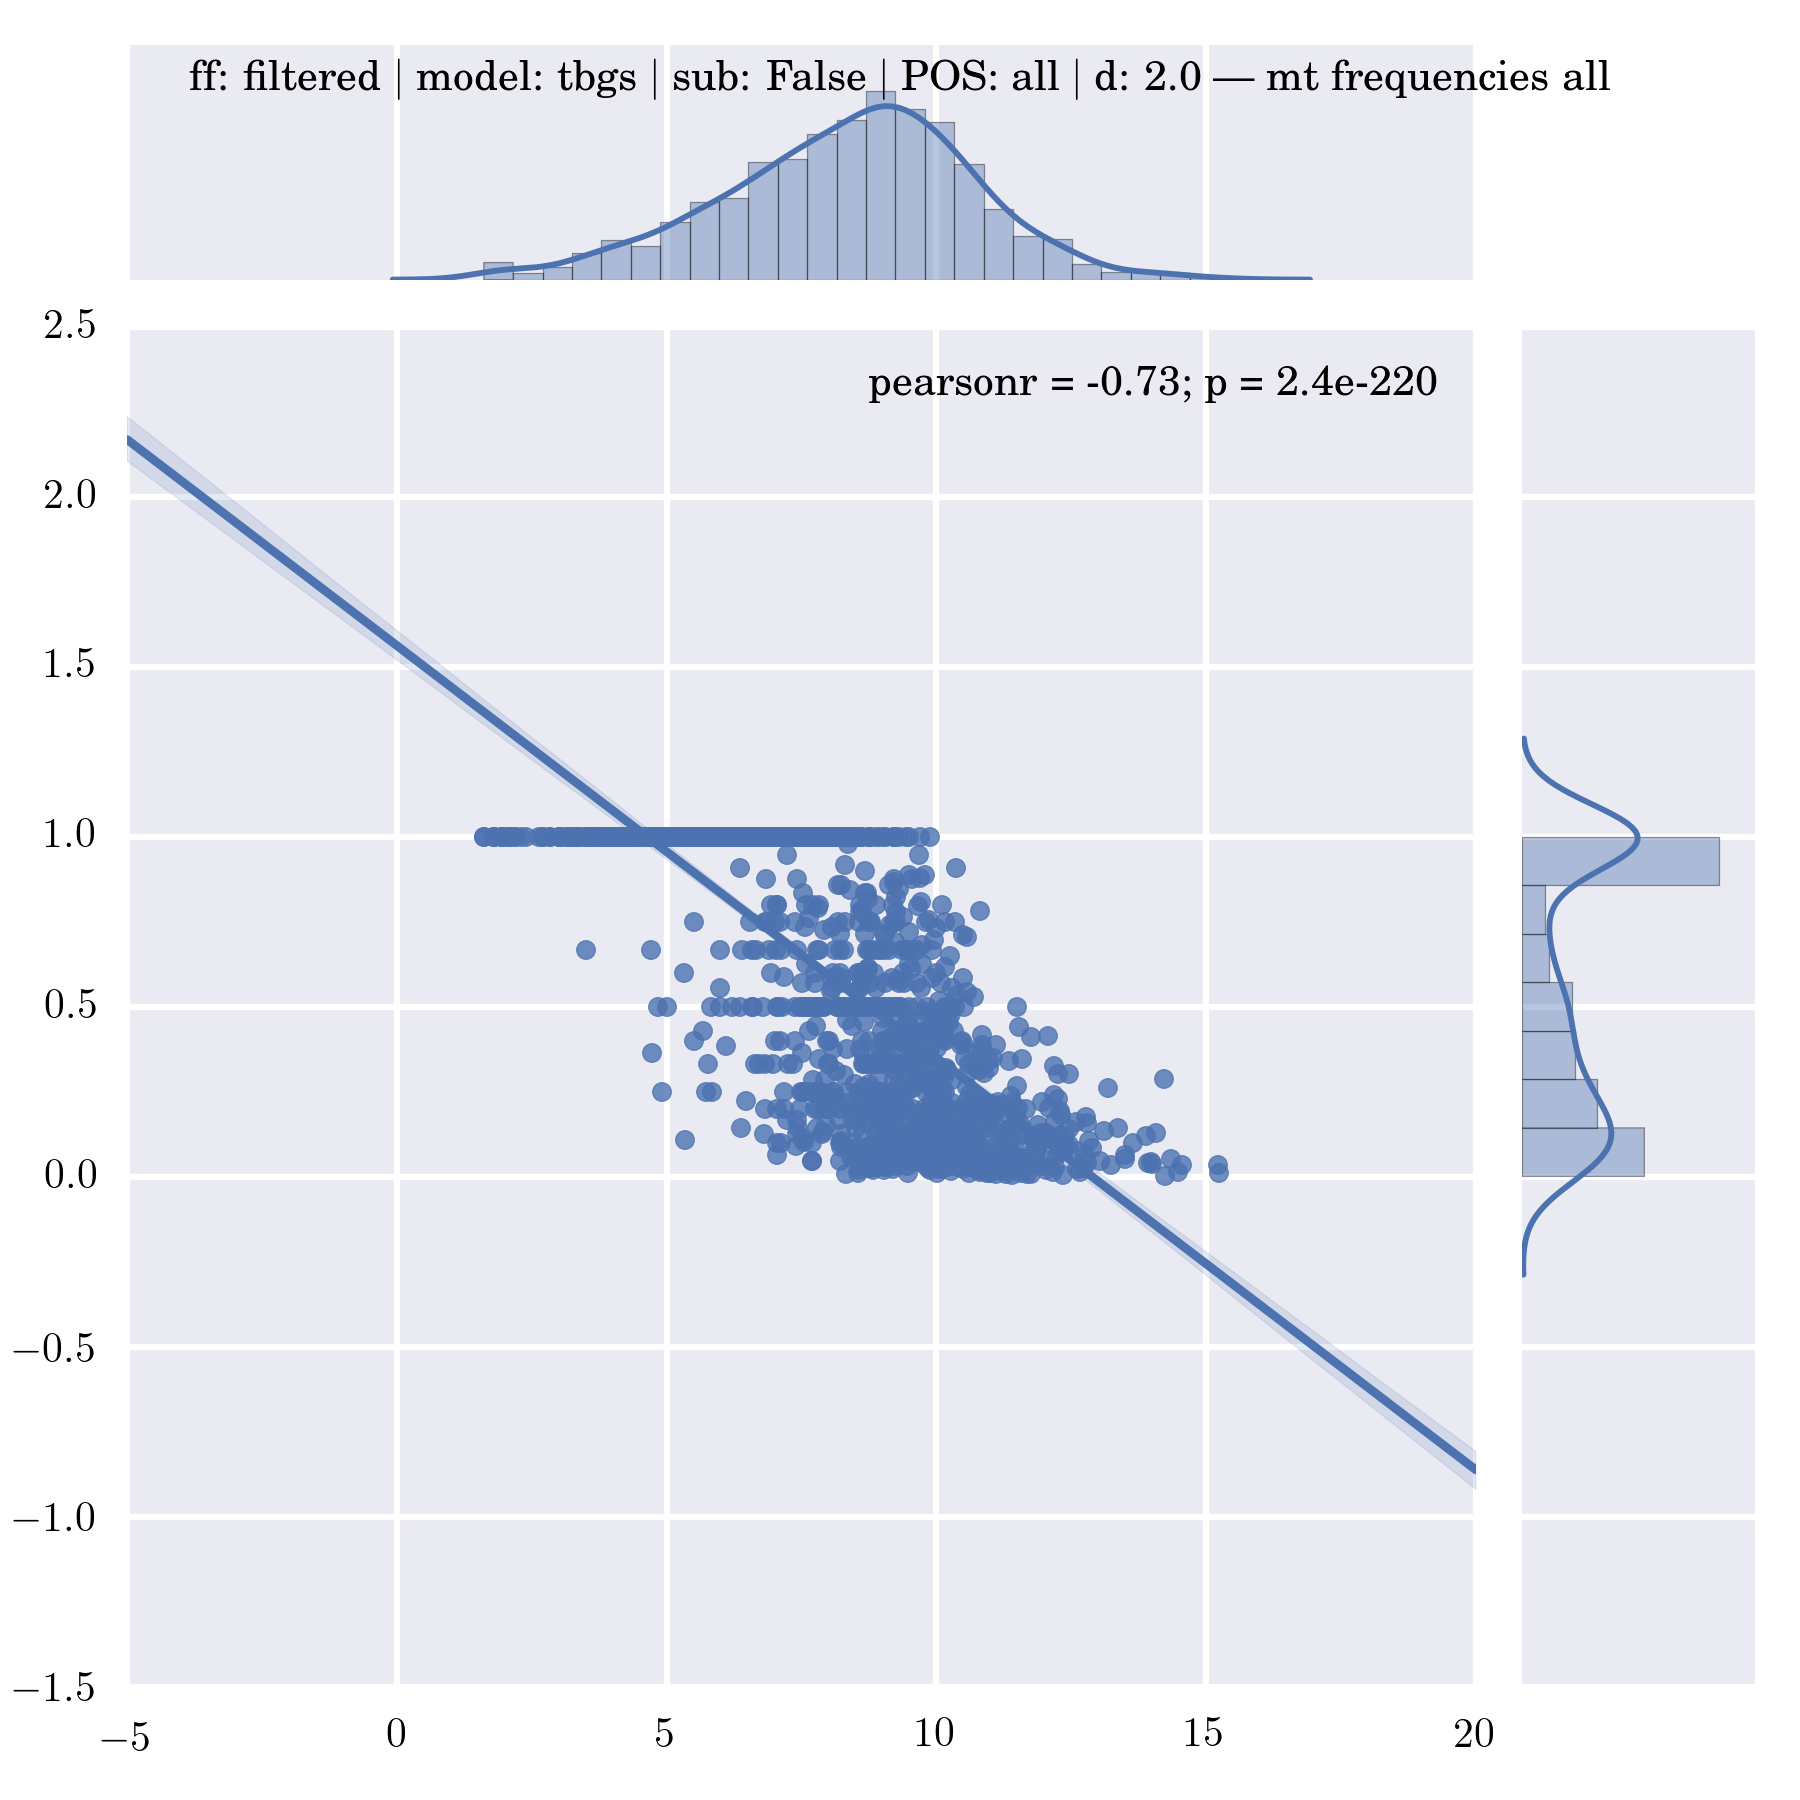
\includegraphics[width=0.3\textwidth]{images/feature-cards/mt_frequencies/susceptibility_scatter.png}
	}
	~
	\subfloat[][Bin averages and KDE]{
		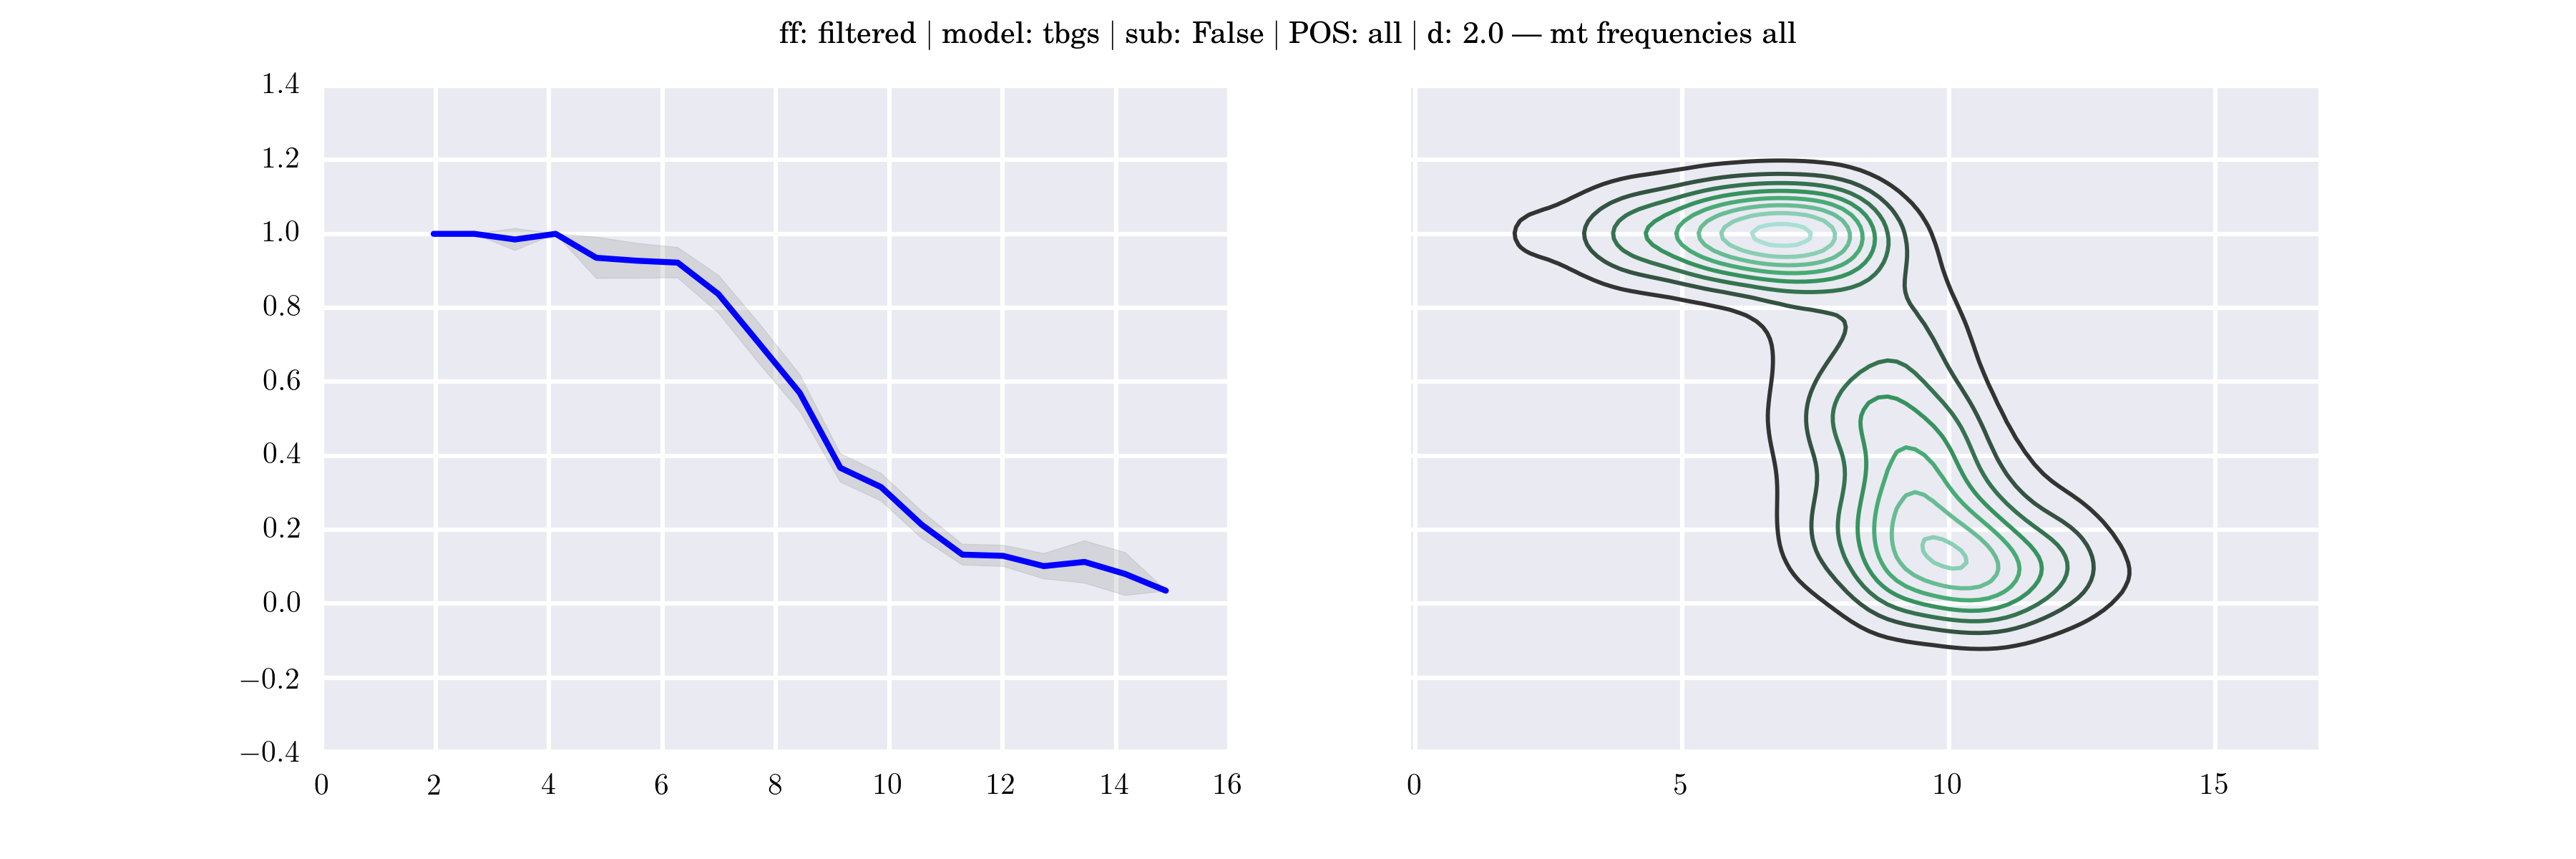
\includegraphics[width=0.6\textwidth]{images/feature-cards/mt_frequencies/susceptibility.png}
	}
	\caption{Substitution susceptibility}
    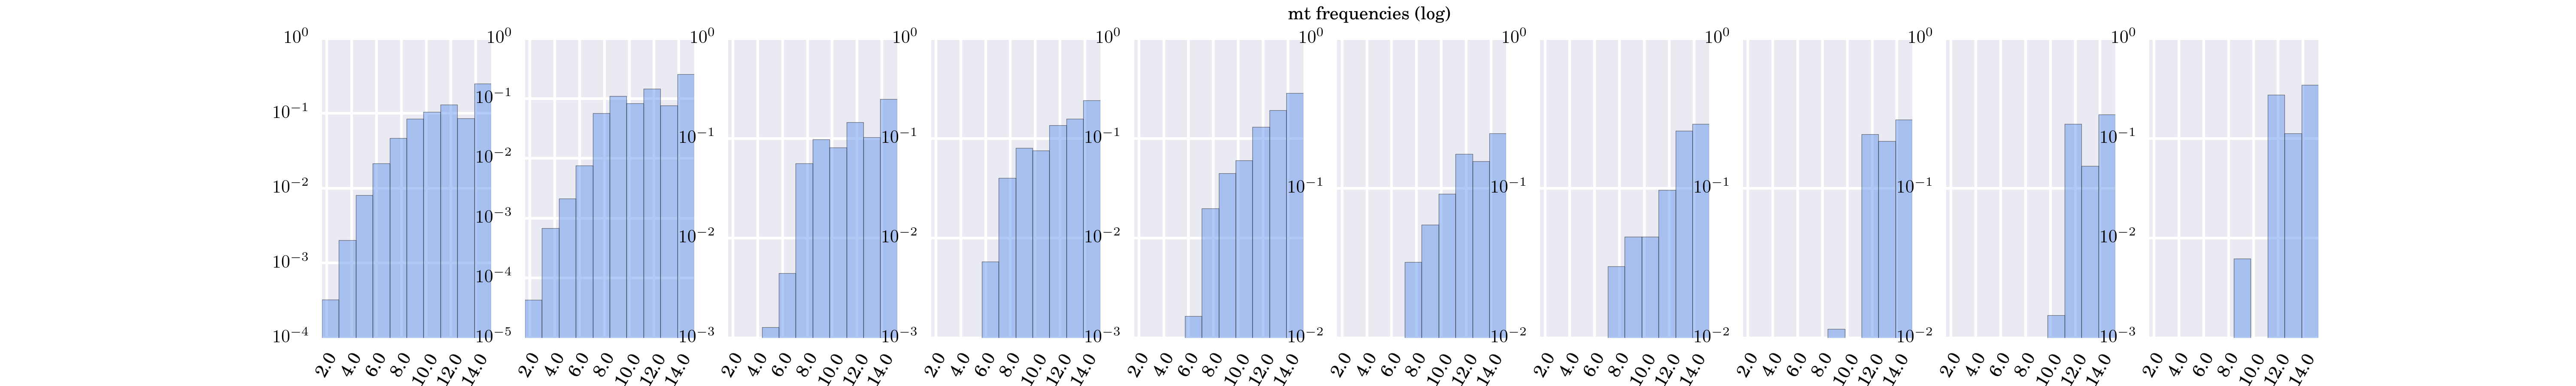
\includegraphics[width=\textwidth]{images/feature-cards/mt_frequencies/timebags_evolution-hist.png}
	\caption{Timebag evolution}
\end{figure*}


% mt_start_frequencies ===============================
\clearpage
\subsection{mt start frequencies}
\begin{figure*}[h!]
    \centering
    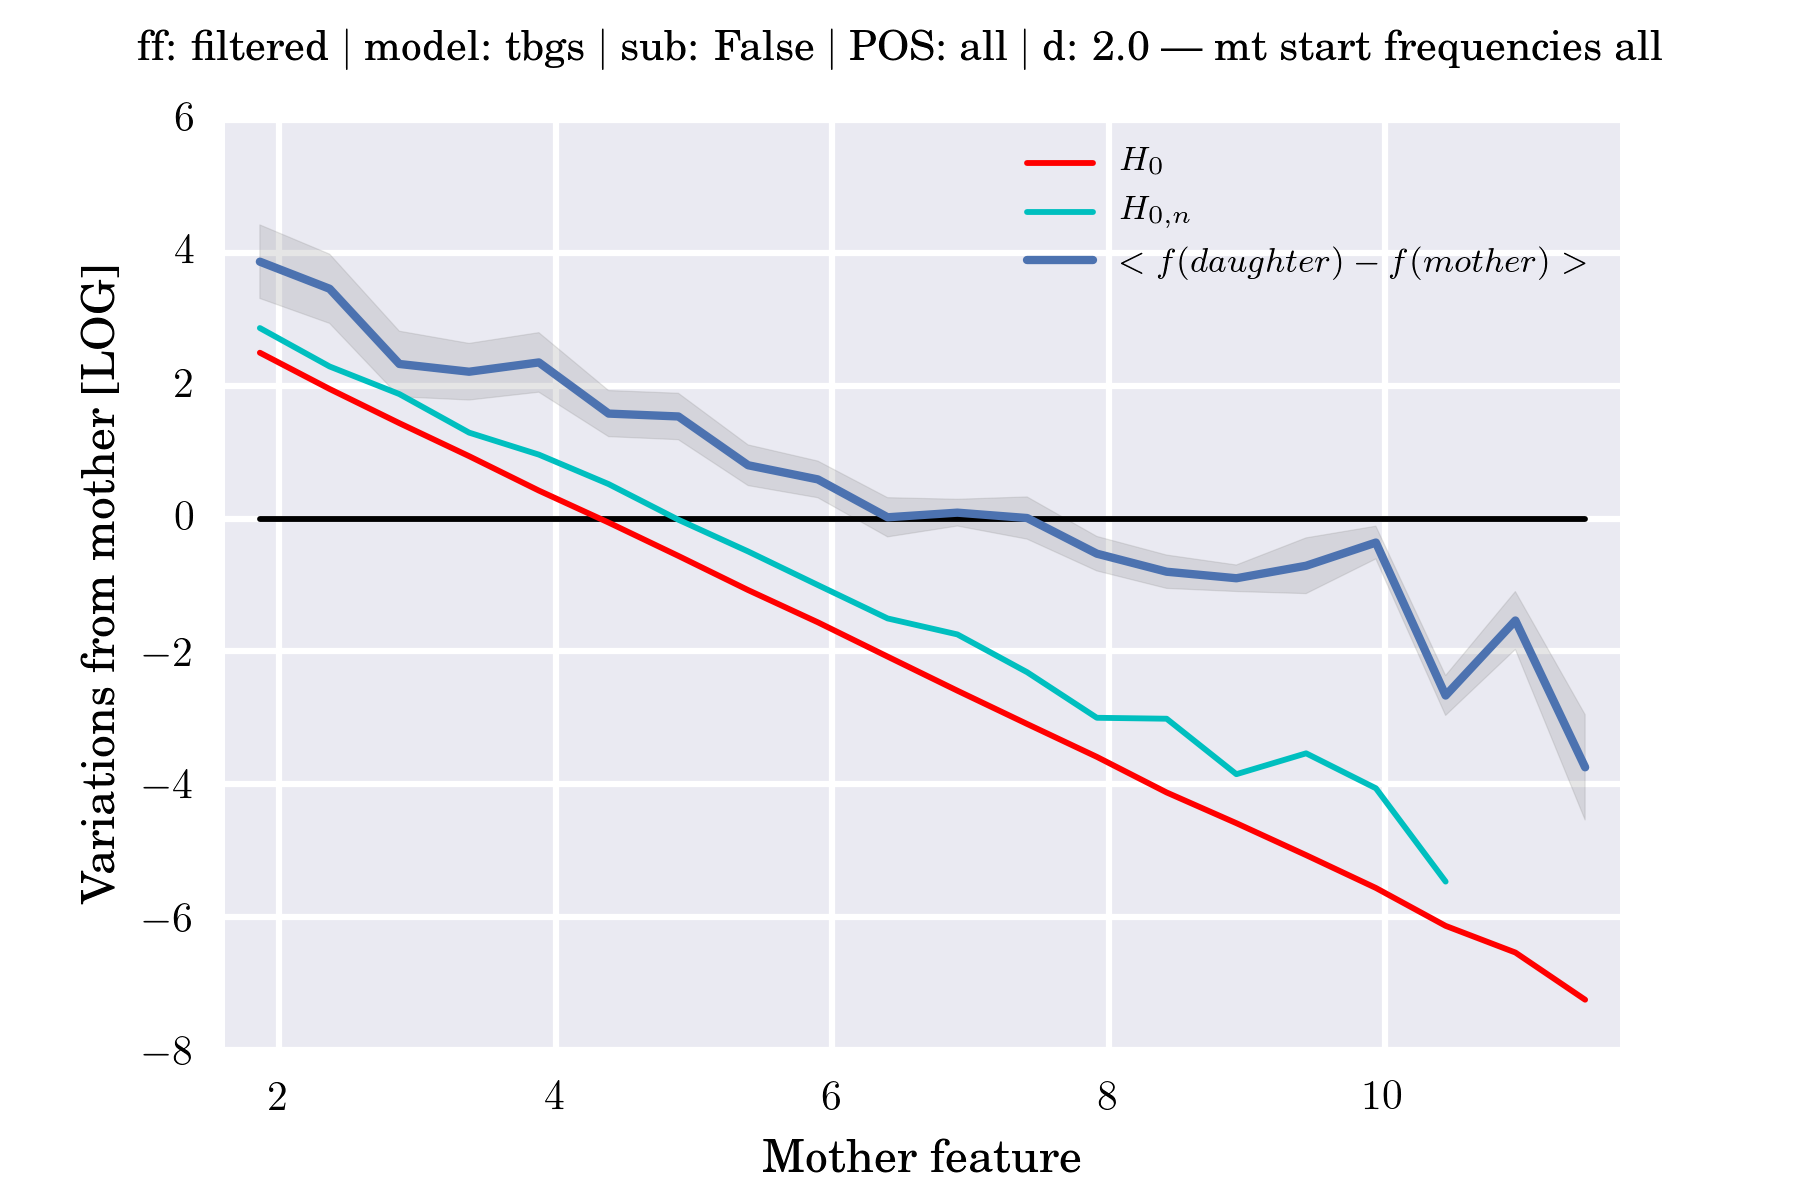
\includegraphics[width=0.6\textwidth]{images/feature-cards/mt_start_frequencies/feature_variations.png}
    \caption{Feature variation on substitution}
	\subfloat[][Scatter plot]{
		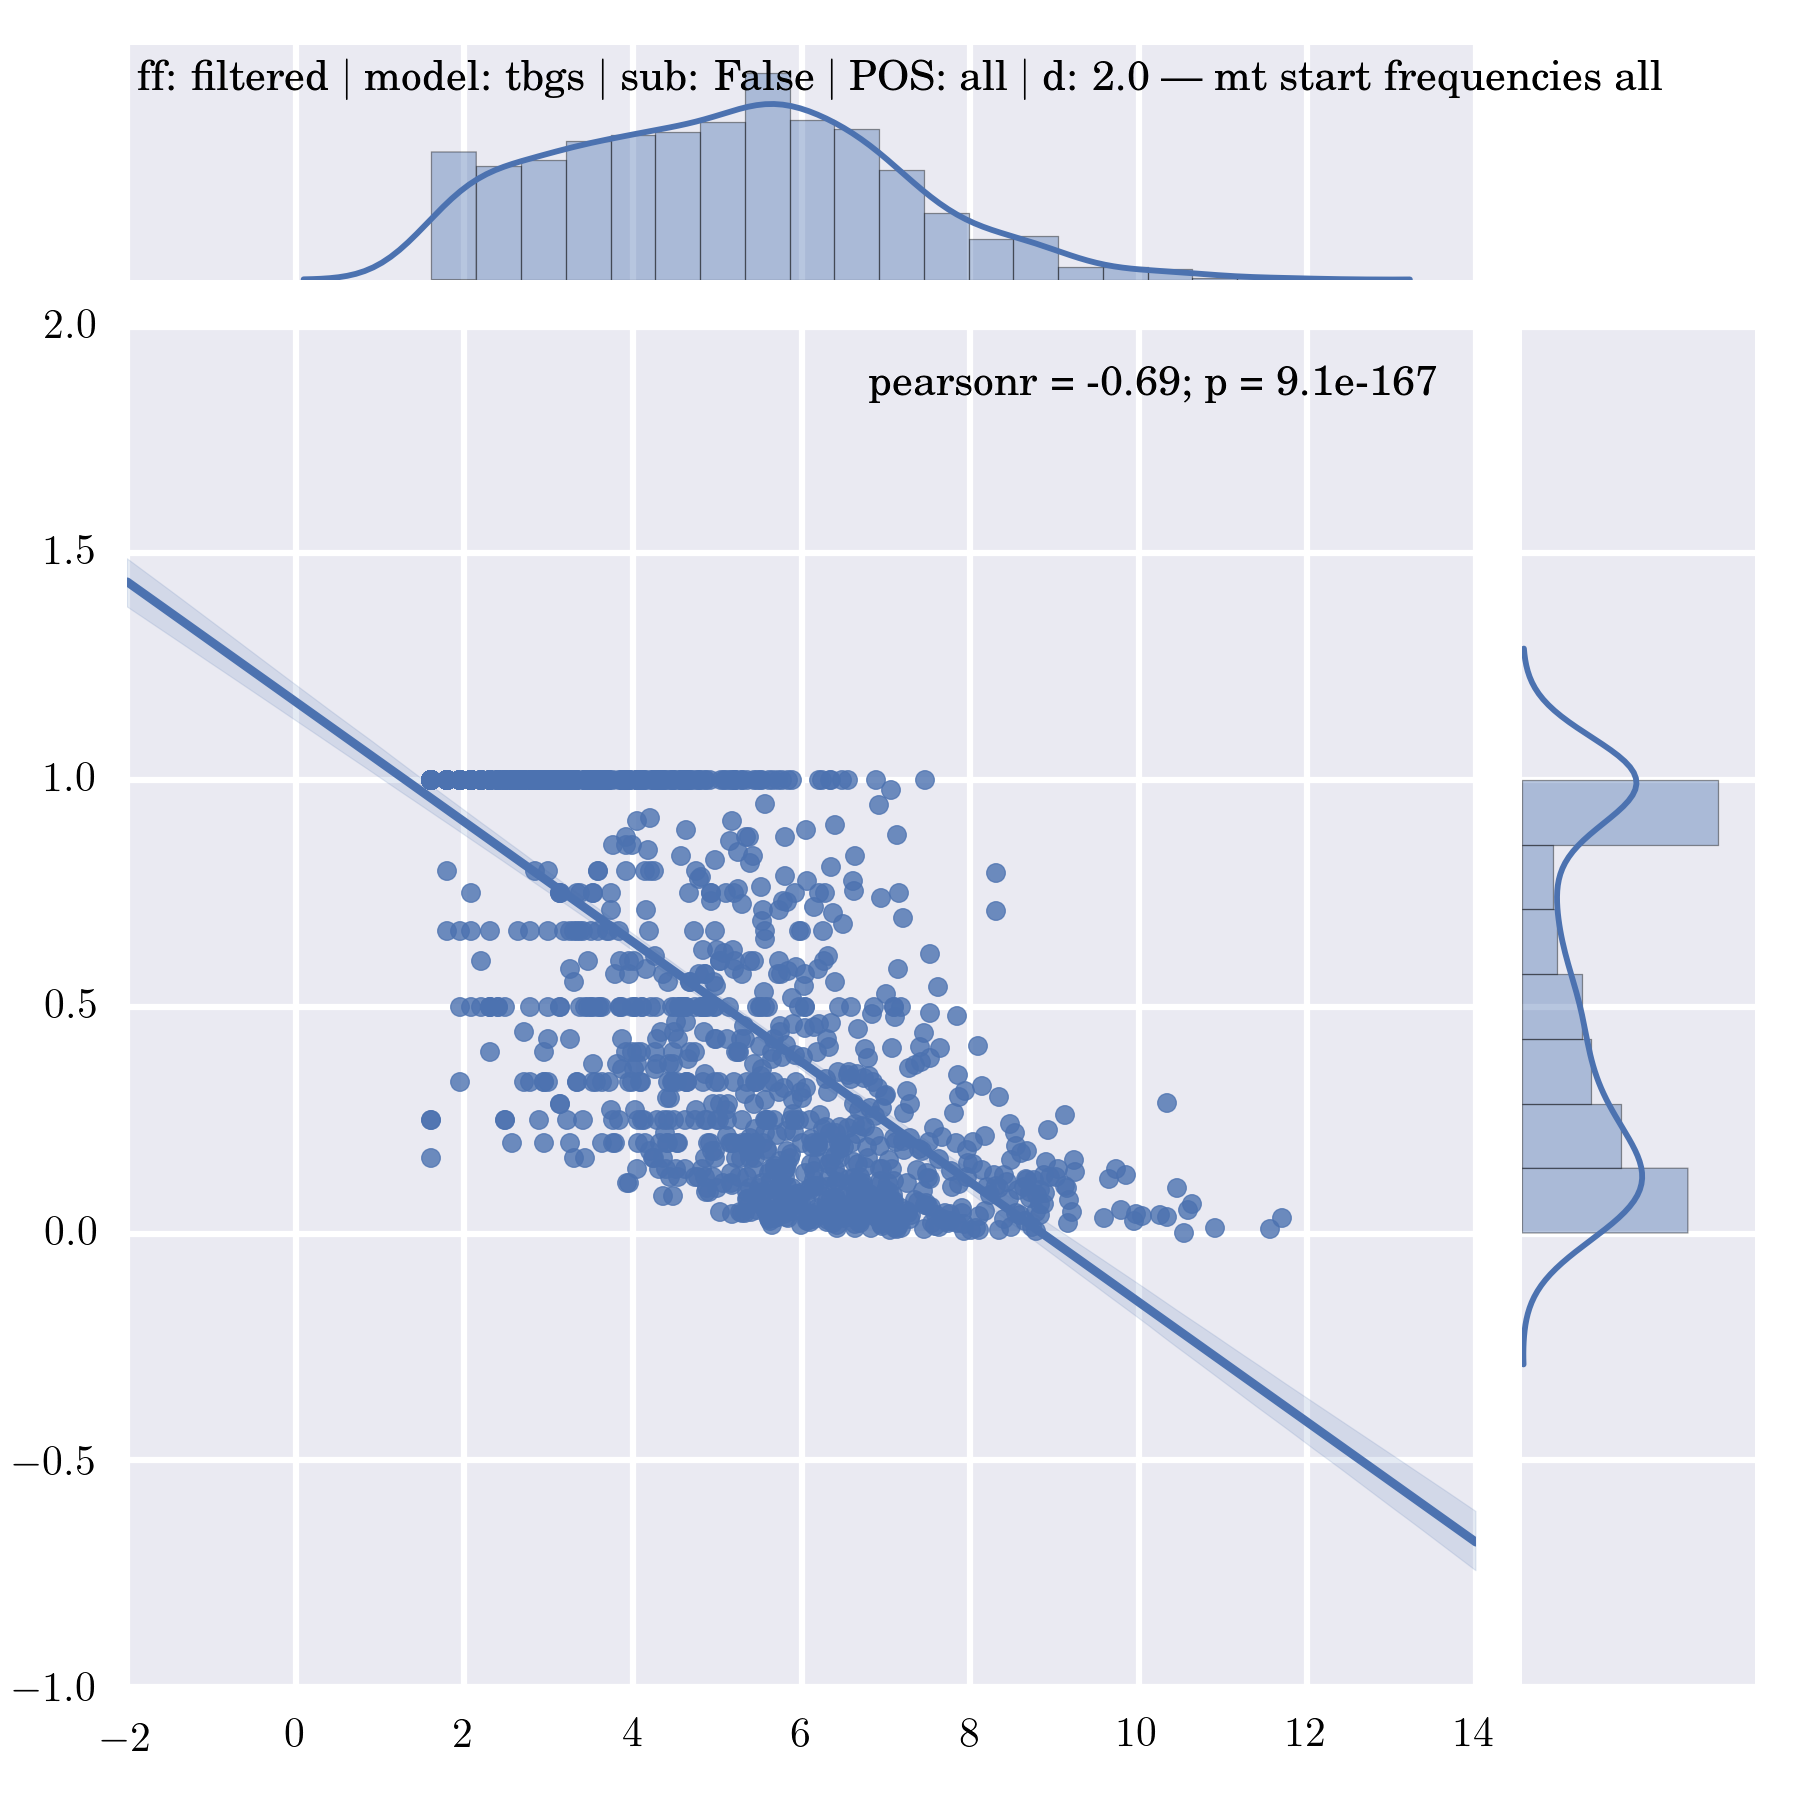
\includegraphics[width=0.3\textwidth]{images/feature-cards/mt_start_frequencies/susceptibility_scatter.png}
	}
	~
	\subfloat[][Bin averages and KDE]{
		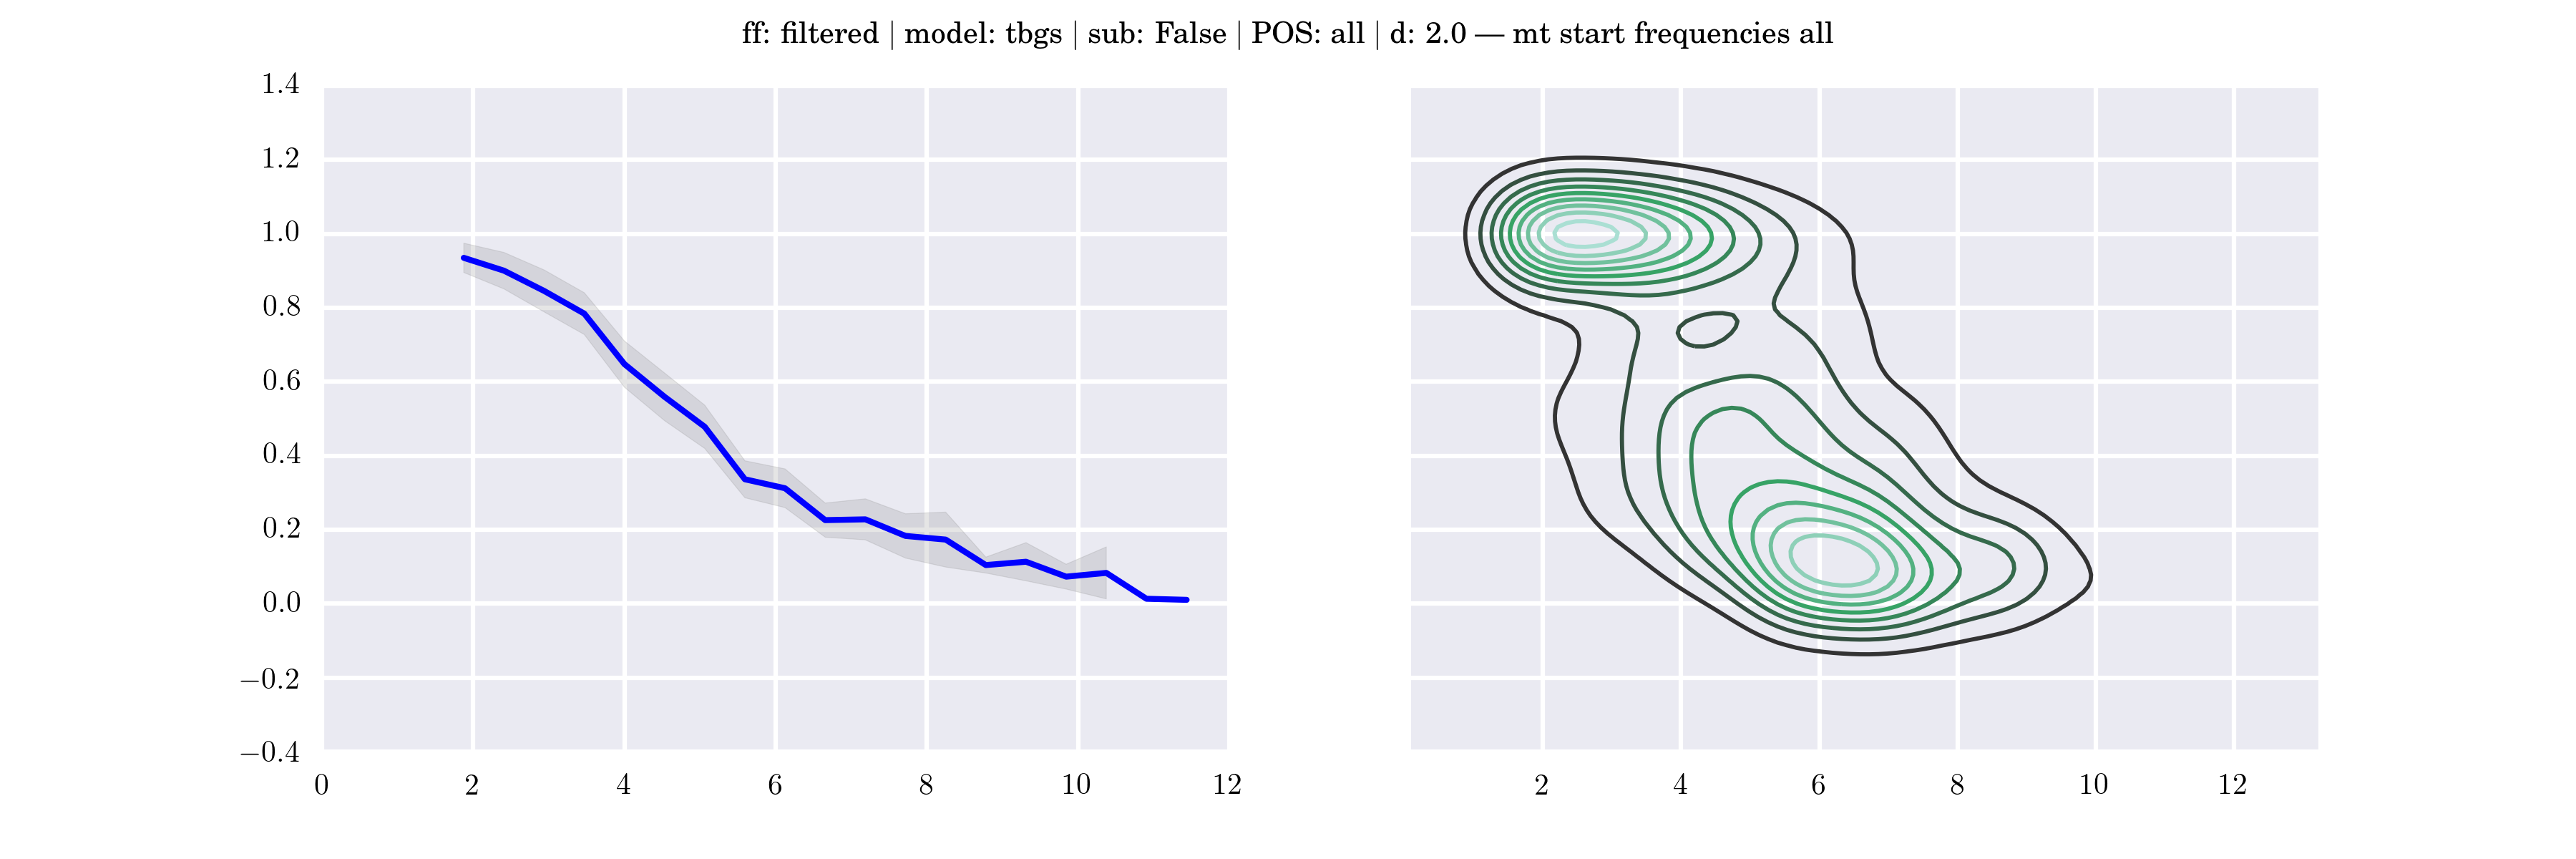
\includegraphics[width=0.6\textwidth]{images/feature-cards/mt_start_frequencies/susceptibility.png}
	}
	\caption{Substitution susceptibility}
    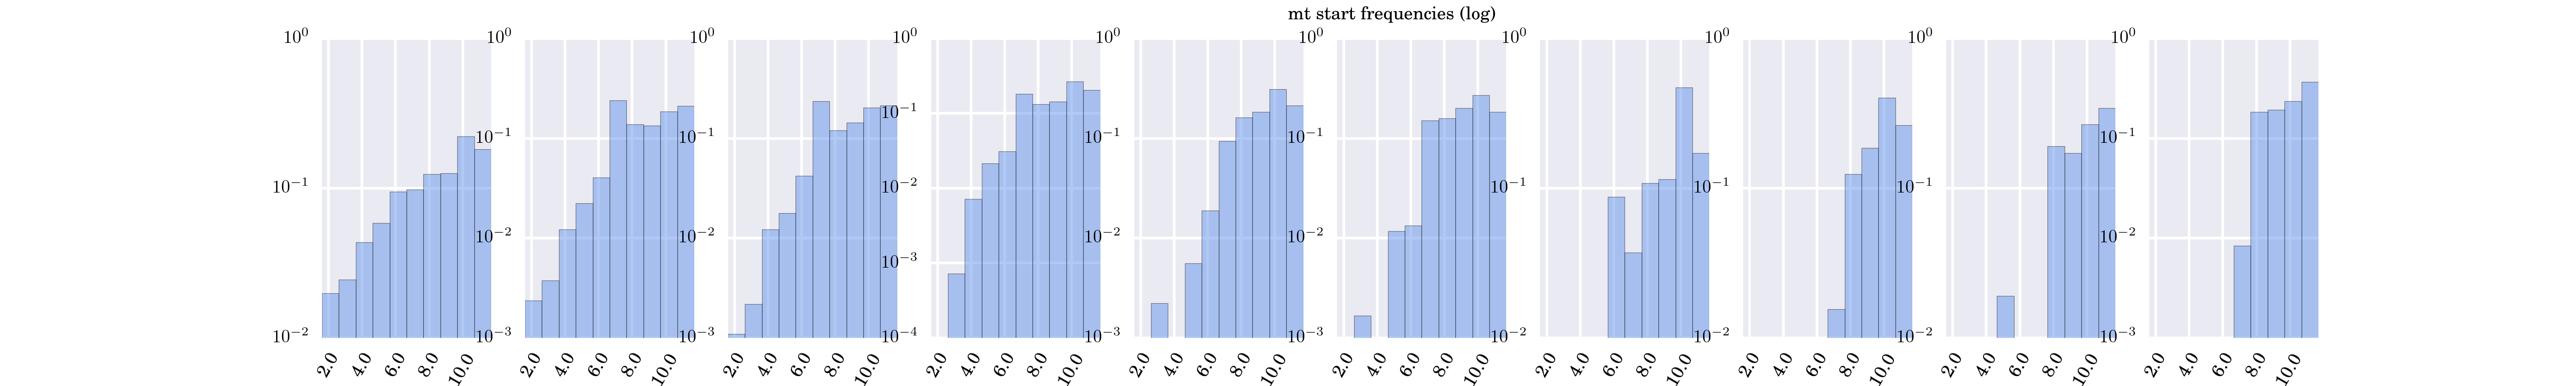
\includegraphics[width=\textwidth]{images/feature-cards/mt_start_frequencies/timebags_evolution-hist.png}
	\caption{Timebag evolution}
\end{figure*}


% wn_BCs ===============================
\clearpage
\subsection{wn BCs}
\begin{figure*}[h!]
    \centering
    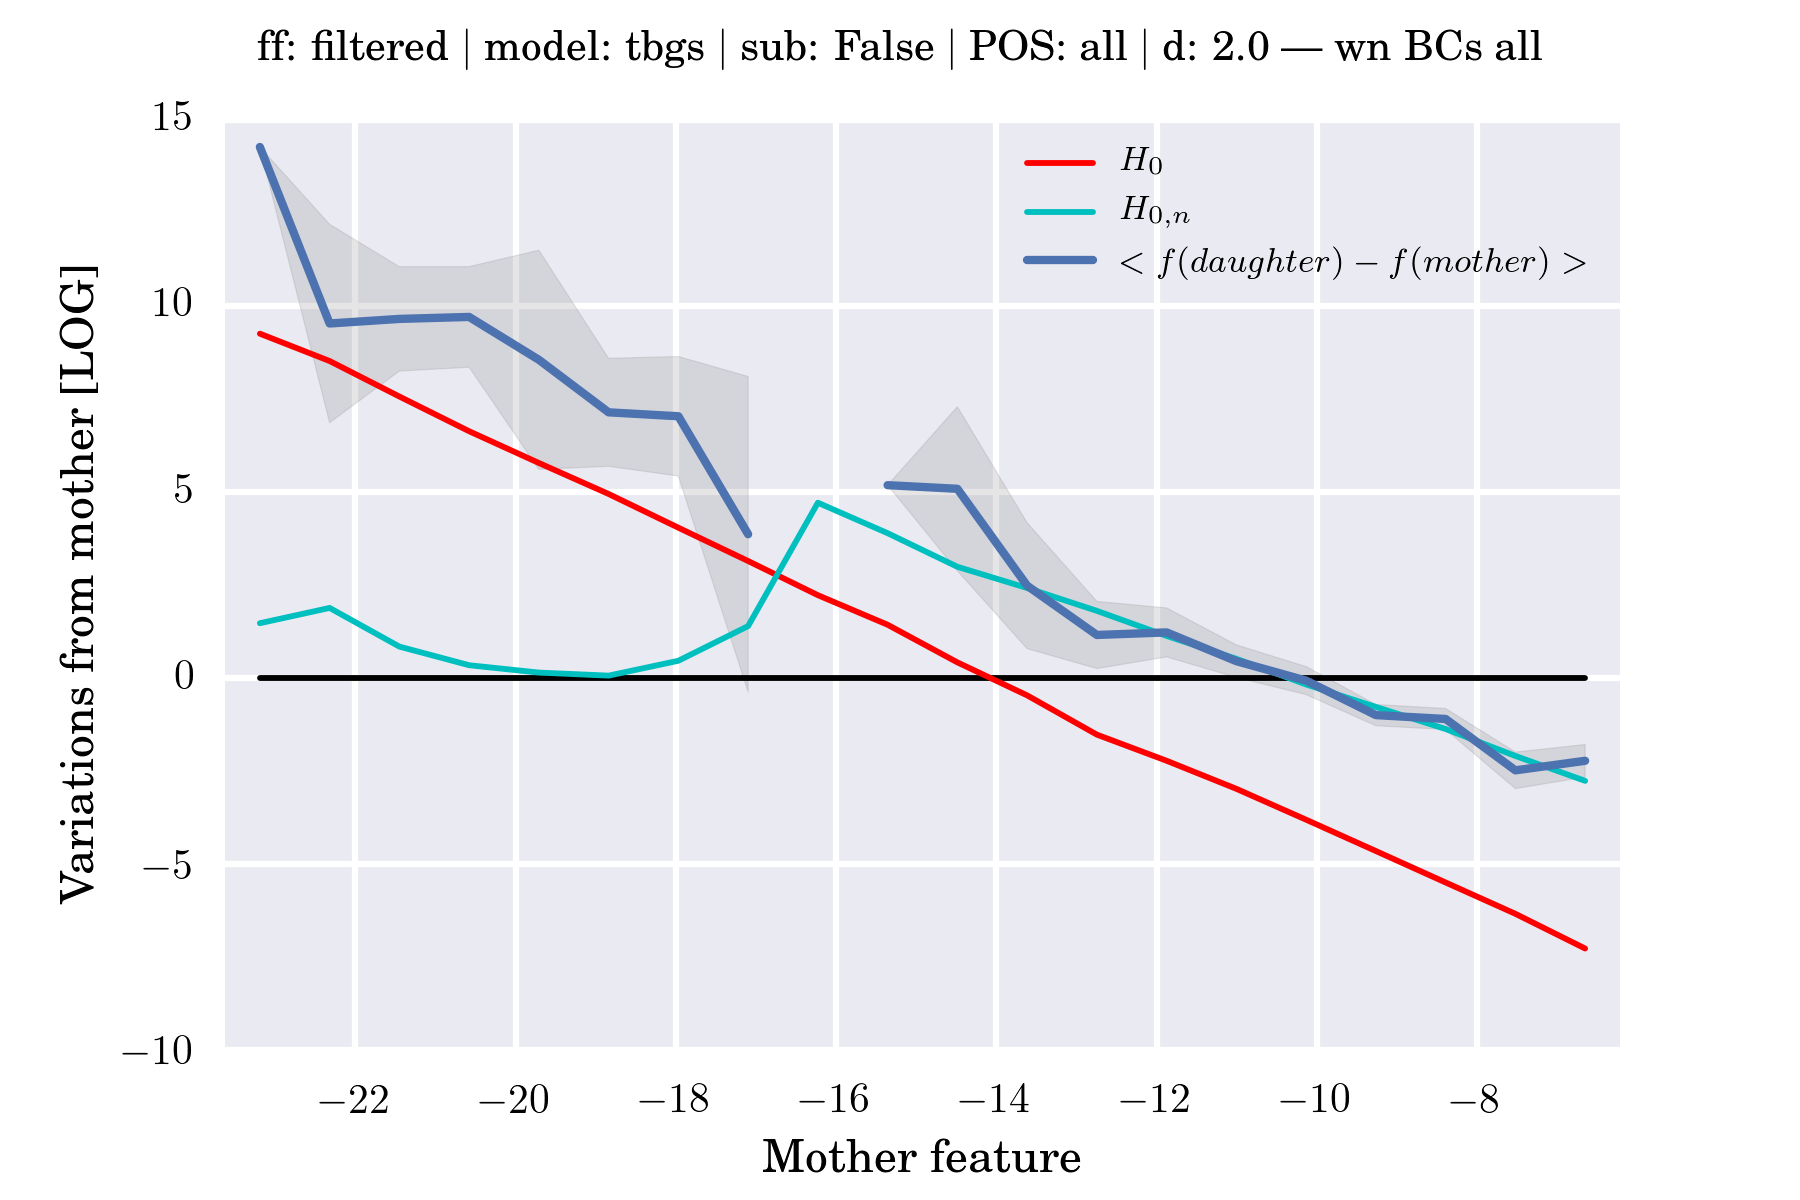
\includegraphics[width=0.6\textwidth]{images/feature-cards/wn_BCs/feature_variations.png}
    \caption{Feature variation on substitution}
	\subfloat[][Scatter plot]{
		\includegraphics[width=0.3\textwidth]{images/feature-cards/wn_BCs/susceptibility_scatter.png}
	}
	~
	\subfloat[][Bin averages and KDE]{
		\includegraphics[width=0.6\textwidth]{images/feature-cards/wn_BCs/susceptibility.png}
	}
	\caption{Substitution susceptibility}
    \includegraphics[width=\textwidth]{images/feature-cards/wn_BCs/timebags_evolution-hist.png}
	\caption{Timebag evolution}
\end{figure*}


% wn_CCs ===============================
\clearpage
\subsection{wn CCs}
\begin{figure*}[h!]
    \centering
    \includegraphics[width=0.6\textwidth]{images/feature-cards/wn_CCs/feature_variations.png}
    \caption{Feature variation on substitution}
	\subfloat[][Scatter plot]{
		\includegraphics[width=0.3\textwidth]{images/feature-cards/wn_CCs/susceptibility_scatter.png}
	}
	~
	\subfloat[][Bin averages and KDE]{
		\includegraphics[width=0.6\textwidth]{images/feature-cards/wn_CCs/susceptibility.png}
	}
	\caption{Substitution susceptibility}
    \includegraphics[width=\textwidth]{images/feature-cards/wn_CCs/timebags_evolution-hist.png}
	\caption{Timebag evolution}
\end{figure*}


% wn_degrees ===============================
\clearpage
\subsection{wn degrees}
\begin{figure*}[h!]
    \centering
    \includegraphics[width=0.6\textwidth]{images/feature-cards/wn_degrees/feature_variations.png}
    \caption{Feature variation on substitution}
	\subfloat[][Scatter plot]{
		\includegraphics[width=0.3\textwidth]{images/feature-cards/wn_degrees/susceptibility_scatter.png}
	}
	~
	\subfloat[][Bin averages and KDE]{
		\includegraphics[width=0.6\textwidth]{images/feature-cards/wn_degrees/susceptibility.png}
	}
	\caption{Substitution susceptibility}
    \includegraphics[width=\textwidth]{images/feature-cards/wn_degrees/timebags_evolution-hist.png}
	\caption{Timebag evolution}
\end{figure*}


% wn_MNSyns ===============================
\clearpage
\subsection{wn MNSyns}
\begin{figure*}[h!]
    \centering
    \includegraphics[width=0.6\textwidth]{images/feature-cards/wn_MNSyns/feature_variations.png}
    \caption{Feature variation on substitution}
	\subfloat[][Scatter plot]{
		\includegraphics[width=0.3\textwidth]{images/feature-cards/wn_MNSyns/susceptibility_scatter.png}
	}
	~
	\subfloat[][Bin averages and KDE]{
		\includegraphics[width=0.6\textwidth]{images/feature-cards/wn_MNSyns/susceptibility.png}
	}
	\caption{Substitution susceptibility}
    \includegraphics[width=\textwidth]{images/feature-cards/wn_MNSyns/timebags_evolution-hist.png}
	\caption{Timebag evolution}
\end{figure*}


% wn_NSigns ===============================
\clearpage
\subsection{wn NSigns}
\begin{figure*}[h!]
    \centering
    \includegraphics[width=0.6\textwidth]{images/feature-cards/wn_NSigns/feature_variations.png}
    \caption{Feature variation on substitution}
	\subfloat[][Scatter plot]{
		\includegraphics[width=0.3\textwidth]{images/feature-cards/wn_NSigns/susceptibility_scatter.png}
	}
	~
	\subfloat[][Bin averages and KDE]{
		\includegraphics[width=0.6\textwidth]{images/feature-cards/wn_NSigns/susceptibility.png}
	}
	\caption{Substitution susceptibility}
    \includegraphics[width=\textwidth]{images/feature-cards/wn_NSigns/timebags_evolution-hist.png}
	\caption{Timebag evolution}
\end{figure*}


% wn_PR_scores ===============================
\clearpage
\subsection{wn PR scores}
\begin{figure*}[h!]
    \centering
    \includegraphics[width=0.6\textwidth]{images/feature-cards/wn_PR_scores/feature_variations.png}
    \caption{Feature variation on substitution}
	\subfloat[][Scatter plot]{
		\includegraphics[width=0.3\textwidth]{images/feature-cards/wn_PR_scores/susceptibility_scatter.png}
	}
	~
	\subfloat[][Bin averages and KDE]{
		\includegraphics[width=0.6\textwidth]{images/feature-cards/wn_PR_scores/susceptibility.png}
	}
	\caption{Substitution susceptibility}
    \includegraphics[width=\textwidth]{images/feature-cards/wn_PR_scores/timebags_evolution-hist.png}
	\caption{Timebag evolution}
\end{figure*}


\end{document}
